%&../.preamble
\endofdump
\graphicspath{{Images}}

\title{Analisi 1}
\author{Mattia Marini}
\date{12.09.22}

\begin{document}

\maketitle
\tableofcontents
\listoftheorems
\listofformulas
\listofincomprensioni
\listofdefs
\newpage
\section{Introduzione}

\label{sec:lezione1}
Romeo Brunetti(progesssore): \textit{romeo.brunetti@unitn.it}\\
Valentino Abram(esercitatore): \textit{valentino.abram@unitn.it}

\begin{minipage}[t]{0.48\textwidth}

	\subsection{Argomenti corso}
	\label{sub:argomentilezioni}
	\begin{itemize}
		\item Continuità
		\item Derivabilità
		\item Integrabilità
	\end{itemize}
\end{minipage}
%
\begin{minipage}[t]{0.48\textwidth}
	\subsection{Argomenti esercitazioni}
	\label{sub:argomentiesercitazioni}
	\begin{itemize}
		\item Esercizi per casa
		\item Esercizi Ddi autovalutazione
	\end{itemize}

\end{minipage}

\subsection{Moodle}
\label{sub:moodle}
\textbox{Tutto ciò che viene affrontato sta sul sito \textbf{moodle}. Ci si arriva da esse3}

\subsection{Libri di testo}
\label{sub:libriditesto}
\begin{itemize}
	\item Canuto e Tabacco - Pearson - Analisi 1
\end{itemize}

\subsection{Esami}
\label{sub:esami}
\begin{itemize}
	\item Solo scritti
	\item 2 esami preliminari (5 novembre, 21 dicembre) + 5 scritti annuali
	\item Se si passa primo preliminare non si passa NON si può fare il secondo
	\item Se entrambi i preliminari vanno bene si può decidere di accettare un voto che è media pesata fra questi due anziche fare i 5 esami canonici
	\item 15 domande a risposta multipla con 2 ore di tempo
	\item Ogni esercizio vale 2 punti, \textbf{risposta errata = -0.4}
	\item Portare \textbf{carta di identità}
	\item Scrivere nome cognome e matricola su foglio di bella
	\item Sono concessi \textbf{talvolta} i formulari: 1 foglio A4 con tips
\end{itemize}

\section{Insiemistica}
\label{sec:insiemistica}
\textbox{Per dare una definizione di insieme rigorosa serve matematica molto complessa. Noi useremo definizione "ingenua"}
\begin{forest}
	[2 definizioni di insieme, for tree={forked edges, draw=gray!20, align=left, grow'=0}
			[Per elenco: enumero nomi oggetti]
			[Per proprietà: es. tutti gli studenti unitn mancini]
	]
\end{forest}


Per elenco: \[
	A = \left\{ b, \beta, A, Brunetti \right\}
\]
\textbox{OSS:  le ripetizioni non contano: $\left\{ a,a,a,b,b,b \right\} = \left\{ a,b \right\} $}

Per proprietà:
\[
	A = \left\{ \text{tutti gli studenti mancini} \right\}
\]
\subsection{Simboli}
\label{sub:simboli}

\subsubsection{Appartiene} \quad A sinistra va l'elemento, a destra l'insieme
\[
	\underbrace{b}_{elemento} \in \underbrace{A}_{insieme}
\]
\subsubsection{Contenuto} \quad B è contenuto o uguale a A
\[
	B \subseteq B
\]
\subsubsection{Strettamente contenuto} \quad A è contenuto ma diverso da B
\[
	A \subsetneq B
\]
\subsubsection{Unione}
\[
	A \cup B = \left\{ x\underbrace{:}_{\text{tale che}} \quad  x \in A \underbrace{\text{ oppure }}_{V} x \in B \right\}
\]
\subsubsection{Intersezione}
\[
	A \cap B \left\{ x : \quad x \in A \text{ e } x \in B \right\}
\]
\subsubsection{Differenza}
\[
	A \setminus     B \left\{ x: \quad x \in a \text{ e } x \not\in B \right\}
\]
\subsubsection{Differenza simmetrica}

\begin{align*}
	A \triangle B & = A \cup B                                                                            \\
	              & = \left\{  x: \quad  x \in A \text{ XOR }\right\}                                     \\
	              & = \left\{ \left( A \setminus B  \right)  \cup \left( B \setminus A \right)   \right\}
\end{align*}
\subsection{Insieme delle parti}
\label{sec:insiemedelleparti}
\textbox{Dato un insieme A si indica con P(A) l'insieme costituito da tutti i sottoinsiemi di A (compresi l'insieme vuoto e A stesso)}
\[
	A = \left\{ 1,2,3 \right\}
\]
\[
	P(A) = \left\{ \left\{ 1,2,3 \right\}, \emptyset , \left\{ 1 \right\}, \left\{ 2  \right\} , \left\{ 3 \right\} , \left\{ 1,2 \right\} , \left\{ 1,3 \right\} , \left\{ 2,3 \right\}   \right\}
\]
\textbox{OSS: L'insieme vuoto è contenuto in ogni insieme}
\textbox{OSS: Se un elemento di un insieme è un insieme, questo va trattato come insieme}

\subsection{Prodotto cartesiano}
\label{sec:prodottocartesiano}
\textbox{Si dice prodotto cartesiano e di indica con $A \times B$ l'insieme delle coppie (a,b) in cui $a \in A$ e $b \in B$ ordinate}
Esempio:
\[
	A = \left\{ 1,2 \right\} \quad B= \left\{ 3,4 \right\}
\]
\[
	A \times B = \left\{ \left( 1,3 \right) , \left( 1,4 \right) , \left( 2,3 \right) , \left( 2,4 \right)  \right\}
\]


\subsection{Funzioni fra insiemi}
\label{sec:funzionifrainsiemi}
Consiste di 3 elementi:
\begin{itemize}
	\item Insieme di partenza $A$
	\item Insieme di arrivo $B$
	\item Legge che ad ogni elemento dell'insieme di partenza $A$ associ un unico elemento dell'insieme di arrivo $B$
\end{itemize}
\[
	f: A \rightarrow B \quad \underbrace{f\left( \underbrace{a}_{\text{elemento di A}}\right)}_{\text{Elemento di B}}
\]
\textbox{NB: Affinchè $f$ possa essere definita una funzione, devono essere collegati tutti gli elementi di A e lo stesso elemento in A non può collegarne due diversi in B }
\subsection{Proprietà delle funzioni}
\label{sec:proprietàdellefunzioni}
\subsubsection{Iniettive}
\label{sub:iniettive}
$f: A \rightarrow B$ è iniettiva se ad ogni coppia di elementi distinti di A associo una coppia di elementi distinti di B
\[
	a_1, a_2 \in A \quad a_1 \neq a_2 \Rightarrow f\left( a_1 \right) \neq f\left( a_2 \right)
\]
Stringi stringi \textit{non esistono elementi distinti che "puntano" allo stesso}
\subsubsection{Surgettive}
\label{sub:surgettine}
$f: A \rightarrow B$ è surgettina se ad ogni elemento di B ne è associato almento uno in A
\[
	\forall b \in B \; \exists \; a \in A : f\left( a \right) = b
\]
Stringi stringi \textit{ogni elemento di B deve essere puntato da almeno un elemento di A}
\subsubsection{Bigettive}
\label{sub:bigettive}
$f: A \rightarrow B$ è bigettiva (o corrispondenza biunivoca) se è sia surgettina che iniettiva

NB: Se f è bigettiva allora $\left| A\right| = \left| B\right|$
\subsubsection{Invertibili}
\label{sub:invertibili}
$f: A \rightarrow B$ è invertibile se esiste una funzione $g: B \rightarrow A$ tale che
\[
	g\left( f\left( a \right)  \right) = a \quad  \forall a \in A
\]
oppure
\[
	f\left( g\left( b \right)  \right) = b \quad \forall b \in B
\]
\textbox{NB: $f: A \rightarrow B$ è invertibile se e solo se f è bigettiva}
\subsection{Insiemi numerici}
\label{sec:insieminumerici}

\begin{itemize}
	\item $\mathbb{N}$ numeri naturali $\left\{ 1,2,3,4,5 \right\} $
	\item $\mathbb{Z}$ numeri interi $\left\{ 0,+1,-1,+2,-2 \right\} $
	\item $\mathbb{Q}$ numeri razionali $\left\{ \frac{1}{2}, -\frac{3}{5} \right\} \quad \frac{m}{q} \quad \text{ con } q \neq 0$
	\item $\mathbb{R}$ numeri reali $\left\{ \sqrt{2},  \right\}  $
	\item $\mathbb{C}$ numeri complessi
\end{itemize}

\subsection{Esempi funzioni}
\label{sec:esempifunzioni}
\[
	f: \mathbb{N} \rightarrow \mathbb{N} \quad f\left( n \right) = n+3
\]
Iniettiva ma non biettiva(0,1,2 non vengono usati)
\[
	f: \mathbb{Z} \rightarrow \mathbb{Z} \quad f\left( n \right) = n+3
\]
Iniettiva biettiva e dunque invertibile
\[
	f: \mathbb{N} \rightarrow \mathbb{N} \quad f\left( n \right) = n^2
\]
Iniettiva ma non suriettiva
\[
	f: \mathbb{Z} \rightarrow \mathbb{Z} \quad f\left( n \right) = n^2
\]

\subsection{Immagine e controimmagine}
\label{sec:immagineecontroimmagine}

\bigbox{L'i mmagine di un un sottoinsieme C di A è l'insieme dei punti di B collegati da una funzione  $f A \rightarrow B$ \[
		I_B = \left\{ f\left( a \right) : a  \in  A \right\}
	\]
}
\bigbox{La controimmagine di un sottoinsieme D di B è l'insieme dei punti di A le cui frecce arrivano in D \[
		I^{-1}_A=  \left\{ a  \in  A : f\left( a \right)  \in B \right\}
	\] }

\subsection{Esteremi superiori ed inferiori di un insieme}
\definizione{Estremi superiori e inferiori}{Sia $A  \in \R, \quad A \neq 0$ L'estremo superiore di A si indica con supA e vale:
	\begin{itemize}
		\item $ + \infty$ se A non è limitato superiormente
		\item Il minimo dei maggioranti di A se è limitato superiormente
	\end{itemize}}
NB: supA e infA esistono sempre!
Esempi:
\begin{itemize}
	\item $(3,7]$  \quad sup=7 \quad inf=3 \quad min non esiste \quad max=7
	      i
\end{itemize}
\incomprensione{09:43:11}
\teorema{Esistenza estremo superiore}{Se $A \subset \R \neq \emptyset $ allora supA esiste.}
Dimostrazione:
\begin{itemize}
	\item Se A non è limitato superiormente allora per definizione supA= $+\infty$
	\item Se A è superiormente limitato l'insieme B dei suoi maggioranti \underline{non è vuoto}
	\item Visto che B è "tutto a destra" di a allora esiste un elemento C separatore (assioma di continuità)
	\item \[
		      a \le c \forall a  \in  A \quad \text{ (c è maggiorante) }\rightarrow c \in B
	      \]
	      \[
		      c \le b \forall b  \in  B \text{ (c è minorante di B) }
	      \]
\end{itemize}
\subsection{Caratterizzare i sup e gli inf}
\begin{itemize}
	\item supA = $ + \infty$ se $ \exists a  \in A \text{ t.c. } a\ge M \quad \forall M  \in  \R$
	\item infA = $- \infty$ se $ \exists a  \in  A \text{ t.c. } a \le M \quad \forall M  \in \R$
	\item supA = L $  \in \R$ se:
	      \begin{itemize}
		      \item a è maggiorante
		      \item $ \forall \epsilon > 0 \quad \exists a  \in  A \text{ t.c. } a \ge L-\epsilon$ \\(se sposto di una quantità infinitesimale L verso A , trovo un elemento di A che è maggiore di L)
	      \end{itemize}
\end{itemize}
%
\hr
%
Esempi:
\begin{itemize}
	\item $A = [0,1]  \cup \left( 2,3 \right)  \cup \left\{ 4 \right\} $
	      \begin{itemize}
		      \item infA=minA=0
		      \item supA=maxA=4
	      \end{itemize}
\end{itemize}
\definizione{Grafico di una funzione}{Si dice grafico di $f$ è il sottoinsieme del prodotto $A \times B$ \[
		graf\left( f \right) = \left\{ \left( a,b \right)  \in  A \times B : f\left( a \right)  = b \right\} \quad \text{ per proprietà }
	\]
	\[
		graf\left( f \right) = 	\left\{ \left( a, f\left( a \right)  \right) : a  \in A \right\} \quad \text{ per elenco }
	\] }
\subsection{Intervalli}
\label{sec:dd}
\[
	\left[ a,b \right] = \left\{ x  \in  \R : a \le x \le b \right\}
\]
Limitato con massimo e minimo
\[
	[a,b) = \left\{ x  \in R : a \le x < b \right\}
\]
Limitato con minimo ma senza massimo
\[
	\left( a,b \right) = \left\{ x  \in  R : a<x<b \right\}
\]
Limitato ma senza massimo e minimo

\section{Principio di induzione}
\label{sec:principiodiinduzione}
\textit{Principio che non si può dimostrare e necessita di due ingredienti}
\begin{itemize}
	\item Insieme dei numeri naturali $\N$
	\item $P_n = \text{affermazione che contenga al suo interno un paramentro} n  \in \N$ che sia vera o falsa
\end{itemize}
Esempi:
\begin{itemize}
	\item $n^2= n+6$ \rarr vera solo per $n=3$
	\item $2^{n} \ge n+6$ \rarr vera per $n \ge 4$ \rarr necessita principio di induzione
	\item Se A contene n elementi allora $P\left( a \right) $ contiene $2^{n}$ elementi
\end{itemize}
Principio di induzione consiste in due passi fondamentali:
\begin{itemize}
	\item \textit{Passo base}Supponiamo che l'affermazione $P_0$ sia vera
	\item \textit{Passo intuitivo}Per qualsiasi $n  \in  \N$ Se $P_n$ è vera, allora $P_{n+1}$ è vera
	\item Allora $P_n$ è vera  $\forall n  \in  \N$
\end{itemize}
\textbox{NB: il punto di partenza \textbf{conta}}
\begin{itemize}
	\item \textit{Passo base} \quad  Supponiamo che l'affermazione $P_{2022}$ sia vera
	\item \textit{Passo intuitivo} \quad Per qualsiasi $n  \in  \N$ Se $P_n$ è vera, allora $P_{n+1}$ è vera
	\item Allora $P_n$ è vera  $\forall n  \in  \left[ 2022, \infty \right] $. Devo controllare manualmente che sia vera anche per $\left[ 0, 2022 \right]$
\end{itemize}
\textbox{NB: la dimostrazione procede come cascata del domino}
\begin{itemize}
	\item \textit{Passo base} \quad Supponiamo che l'affermazione $P_{2022}$ sia vera
	\item \textit{Passo intuitivo} \quad Per qualsiasi $n  \in  \N$ Se $P_n$ è vera, allora $P_{n+1}$ è vera $\forall n \ge 1$
	\item Dimostrazione non procede perchè paso base non vale per n=0
\end{itemize}
%
\hr
%
\subsection{Dimostrazione 1}
\label{sub:dimostrazione1}
Dimostrazione che $\sum_{k=0}^{n} k = \frac{n\left( n+1 \right) }{2}$
\begin{itemize}
	\item \textit{Passo base} Verifico che $P_0$ è vera \rarr basta sostituire $0= \frac{0\cdot 1}{2}$
	\item Visto che $P_n$ è vera per \textit{hp} scrivo che \[
		      \underbrace{\left[ 0+1+2+3\ldots+n \right] +\left( n+1 \right)}_{_{\text{somma dei primi n+1 numeri}}} = \frac{n\left( n+1 \right) }{2} + \left( n+1 \right)
	      \]
	\item Raccolgo a destra e ottengo
	      \[
		      \sum_{k=0}^{n+1} k = \frac{\left( n+2 \right) \left( n+1 \right) }{2}
	      \]
\end{itemize}

\textbox{In alternativa posso usare il metodo di gauss per verificare questa hp. (Divido i numeri da 0 a n in due e li sovrappongo al contrario)}

\subsection{Dimostrazione 2}
\label{sub:dimostrazione2}
Dimostrazione che $\sum_{k=0}^{n} k^2 = \frac{n\left( n+1 \right) \left( 2n+1 \right) }{6} $
\begin{itemize}
	\item \textit{Passo base} $\sum_{k=0}^{0} k^2 = \frac{0 \cdot 1 \cdot 1}{6} = 0$
	\item \[
		      \underbrace{\left[0^2 + 1^2 + 2^2 + 3^2 + 4^2 \ldots n^2\right]}_{\text{Ho dimostrato quanto vale in passo base}} \left( n+1 \right)^2 = \underbrace{\frac{n\left( n+1 \right) \left( 2n+1 \right) }{6}} + \left( n+1 \right)^2
	      \]

	      \begin{align*}
		      f \left( n \right)                                                  & = \frac{\left( n+1 \right) \left( 2n+1 \right)}{6}                                       \\
		      f\left( n+1 \right)                                                 & = \frac{\left( n+1 \right) \left( n+2 \right) \left( 2n+3 \right)}{6}                    \\
		      f\left( n+1 \right)                                                 & = f\left( n \right) +\left( n+1 \right) ^2                                               \\
		      \frac{\left( n+1 \right) \left( n+2 \right) \left( 2n+3 \right)}{6} & = \frac{\left( n+1 \right) \left( n\left( 2n+1 \right) +6\left( n+1 \right)  \right)}{6} \\
		      \left( n+1 \right) \left( 2n^2 + 7n + 6 \right)                     & = \left( n+1 \right) \left( 2n^2 + 7n +6 \right)
	      \end{align*}

	\item Applico algebra e dimostro che
	      \[
		      \sum_{k=1}^{n} k^2 = \frac{n\left( n+1 \right) \left( 2n+1 \right)}{6}
	      \]

\end{itemize}
\subsection{Dimostrazione 3}
\label{sub:dimostrazione3}

Dimostrazione che $\sum_{k=1}^{n} a^{k} = \frac{a^{n+1}-1}{a-1}$
\begin{itemize}
	\item \textit{Passo base} $1=\frac{a-1}{a-1}$
	\item \[
		      \left[ 1+a+a^2 \ldots a^{k+1} \right]= \frac{a^{n+1}-1}{a-1} + \left( a \right) ^{n+1}
	      \]
\end{itemize}
\subsection{Dimostrazione 4}
\label{sub:dimostrazione4}

Dimostrazione che $2^{n} \ge n \quad \forall n  \in  \N$
\begin{itemize}
	\item \textit{Passo base verificato} $2^{0} \ge 0$
	\item \[
		      2^{n+1} \ge n+1 \rightarrow 2 \cdot \underbrace{2^{n}}_{\ge n} \ge n+1
	      \]
	      \[
		      2 \cdot 2 ^{n} \ge 2n \text{ dato che  } 2^{n} \ge n \text{ per hp }
	      \]
	\item Verifico che $2n \ge n+1 \forall \N  \in \left[ 1, \infty \right] $
	      i
\end{itemize}
\subsection{Disuguaglianza di bernulli}
\label{sub:disbernoulli}
\formula{Disuguaglianza di Bernoulli}{
	\[
		\left( 1+x \right) ^{n}\ge 1 + nx \quad \forall n  \in  \N \quad x > -1
	\]
}
\[
\]
\begin{itemize}
	\item \textit{Passo base verificato}
	\item \textit{Passo induttivo} \[
		      \underbrace{\left( 1+x \right) ^{n+1}}_{ \left( 1+x \right) ^{n} \left( 1+x \right) } \ge 1+x\left( n+1 \right)
	      \]
\end{itemize}
\section{Proprietà dei numeri reali}
\label{sec:proprietàdeinumerireali}
\begin{itemize}
	\item Proprietà algebriche
	\item Proprietà ordinamento
	\item Assioma di continuità
\end{itemize}
\subsection{Proprietà algebriche somma}
\label{sub:proprietàalgebriche}
\begin{itemize}
	\item Proprietà commutativa $a+b=b+a \quad \forall a,b  \in \R$
	\item Proprietà associativa $\left( a+b \right) +c = a+ \left( b+c \right) \forall a,b,c  \in  \R$
	\item Esistenza elemento neutro $\exists 0  \in  \R \text{ t.c } a+0=a$
	\item Esistenza elemento opposto $\forall a  \in  \R \exists b  \in  \R \text{ t.c.} a+b=0$
\end{itemize}
\subsection{Proprietà algebriche prodotto}
\label{sec:proprietàalgebricheprodotto}
\begin{itemize}
	\item Prorpietà commutativa $a \cdot b = b\cdot a \forall a,b  \in  \R$
	\item Proprietà associativa $\left( a\cdot b \right) \cdot c = a \cdot \left( b\cdot c \right) \forall a,b,c  \in  \R$
	\item Esistenza elemento neutro $\exists 1  \in \R \text{ t.c } a\cdot 1=a$
	\item Esistenza elemento opposto $\forall a  \in \left\{ \R-\left\{ 0 \right\}  \right\}  \quad \exists b  \in  \R \text{ t.c. } a\cdot b=0$
	\item Proprietà  distributiva $a\left( b+c \right) = ab+bc$
\end{itemize}
\subsection{Proprietà ordinamento}
\label{sub:proprietàordinamento}
\begin{itemize}
	\item Riflessiva se $x\le x$
	\item Antisimmetrica se $x \le y$ e $x \ge y$ alora $x=y$
	\item Transitiva se $x \le y$ e $y \le z$ alora $x\le z$
	\item se $y \le x$ allora  $zy \le zx \quad \forall z  \in \R^{+}$
\end{itemize}
\subsection{Assioma di continuità}
\label{sub:assiomadicontinuità}\phantom{.}
\assioma{Assioma di continuità}{
	Siano A e B due sottoinsiemi non vuoti dei numeri reali. Supponiamo che ogni elemento di A sia minore o uguale a B. Per quando i due insiemi siano vicini esiste almeno un numero reale che stia fra a e b ossia:
	\[
		\exists c  \in \R \text{ t.c. } \quad a\le c \le b \quad \forall a  \in A, b  \in B
	\]
}

\bigbox{
	\textit{Se C appartiene sia ad A che a B questo elemento è unico}
	NB: l'assioma di continuità vale per i numeri reali $\R$ ma non vale per i razionali $\R$ ad esempio con i due insiemi seguenti
	\begin{gather}
		A = \left\{ x  \in  \R  : x \le 0 e x^2 < 2 \right\} \\
		B = \left\{ x  \in  \R  : x \ge 0 e x^2 > 2 \right\}
	\end{gather}
	Unico elemento separatore è $\sqrt{2} $, numero che è reale
}
NB: c può essere unico nel caso di insiemi che hanno come intersezione c stesso ma anche in insiemi con intersezione vuota: es $R^{-}$ e $R^{+}$
\definizione{Densità degli insiemi}{Siano A e B insiemi non vuoti. Si dice che \underline{A è denso in B} se per ogni elemento $b_1, b_2  \in  B$ esiste un elemento in A tale che $b_1 \le a \le b_2$}
\definizione{Maggiorante e minorante}{Si dice che un numero k reale è un \underline{maggiorante} del sottoinsieme A se $k \ge a \forall a  \in  A$\\
	Si dice che un numero k reale è un \underline{minorante} del sottoinsieme A se $k \le a \forall a  \in  A$
}
NB: maggioranti e minoranti non devono esistere necessariamente ad esempio in $\R^{+}$ o in $ \N $ non esiste maggiorante
\vskip3mm
NB: se esistono, maggioranti e minoranti non sono unici

\definizione{Insiemi limitati superiormente/inferiormente}{Dato un insieme A non vuoto questo di dice limitato superiormente su esiste un suo maggiorante\\
	Dato un insieme A non vuoto questo di dice limitato inferiormente se esiste un suo minorante\\
	Dato un insieme A non vuoto questo di dice limitato se esiste un suo maggiorante e un suo minorante \[
		A  \in \R \quad A \neq \emptyset \text{ è limitato se e solo se } \exists k  \in  \R \text{ t.c. } \left|a\right| \le k \forall a  \in  A
	\]
}
\definizione{Massimo/minimo insieme}{Sia $ A  \in \R$ non vuoto si dice che $ M  \in \R$ è massimo di A e si indica con $M = max\left( A \right) $ se:
	\begin{itemize}
		\item $ a \le M \quad \forall a  \in  A $ ossia M è un maggiorante
		\item $ M  \in A$
	\end{itemize}}
NB: se un insieme ha massimo o minimo, questi sono necessariemente unici


\section{Polinomi}
\label{cha:polinomi}
$ P\left( x \right)$  nella variabile x di grado k è un oggetto del tipo

\[
	p\left( x \right) = a_0 + \sum_{k=1}^{n} a_k z^k
\]
\subsection{Operazioni polinomi}
\label{sec:operazionipolinomi}
\subsubsection{Somma Polinomi}
Considero $P\left( x \right) $ e $Q\left( x \right) $, rispettivamente di grado $n$ e $m$ con $n \le $
\begin{itemize}
	\item Completo $P\left( x \right) $ i modo tale che abbia esponenti fino a m
	      \[
		      P\left( x \right) = \sum_{k=0}^{n} a_k x^{k} + \sum_{k=n+1}^{m} a_k x^{k}
	      \]
	\item Somma è uguale a:
	      \[
		      \left( p+q \right) \left( x \right) = \sum_{k=0}^{n} \left( a_k + b_k \right)  x^k
	      \]
\end{itemize}
\[
	Q\left( x \right) = b_0 + \sum_{k=1}^{n} a_k
\]

\subsubsection{Moltiplicazione}
\label{sub:moltiplicazione}
Dato un polinomio $P\left( x \right)$ e un fattore $k \in  \R$

\subsubsection{Moltiplicazione fra polinmoni}
\label{sub:moltiplicazionefrapolinmoni}
Praticamente applico proprietà distributiva

\subsection{Divisione fra polinomi}
\label{sub:divisionefrapolinomi}
Dato $P\left( x \right) $ e $ Q\left( x \right) $ con $Q\left( x \right) \neq 0$
\[
	f\left( x \right) = \frac{P\left( x \right) }{Q\left( x \right) }
\]
\teorema{Divisione fra polinomi}{Dati due polinomi $ P_1\left( x \right) , P_2\left( x \right)  $ di grado n e m con $n \ge m$ esistono 2 polinomi $ Q\left( x \right)  e R\left( x \right) $ tali che \[
		P_1\left( x \right)  = P_2\left( x \right) Q\left( x \right) + R\left( x \right)
	\]
	Il grado di R è \underline{strettamente minore} del grado di $P_2$
}

\subsubsection{Algoritmo standard divisione}

\begin{itemize}
	\item Scrivo polinomio completo ( $12x^3 + 0 x^2 + x + 6$ )
	\item Divido grado massimo di $\left( P\left( x \right)  \right) $ per grado massimo di $Q\left( x \right) $
	\item Moltiplico risultato ottenuto e sottraggo con ultimo polinomio ottenuto a sx
\end{itemize}
\begin{table}[h!]
	\centering
	\caption{Divisione fra polinomi}
	\label{tab:label}
	\begin{tabular}{r|l}
		$ x^{5} + 0 x^{4}+ 2x^{3} + 0 x^{2} + x + 3$ & $x^{3}+ 3x$                                                           \\
		\hline
		$ x^{5} + 0 x^{4}+ 3x^{3} + 0 x^{2} +0 $     & $ \underbrace{x^{2}}_{\text{Step 1}} \underbrace{-1}_{\text{Step 2}}$ \\
		$ 0 + 0 - x^{3} + 0 + x - 3$                 &                                                                       \\
		$ 0 + 0 - x^{3} + 0 + -3x + 0$               &                                                                       \\
		$ \underbrace{0+0+0+0+4x+3}_{\text{Resto } R\left( 0 \right) } $
	\end{tabular}
\end{table}

\subsubsection{Algoritmo di ruffini}
\label{sec:algoritmodiruffini}
\textit{Algoritmo utilizzabile solo se il divisore è di grado 1, nella forma} $D\left( x \right) = ax + c \text{ con } a = 1$
\begin{itemize}
	\item Scrivo polinomio da dividere completo in alto
	\item Scrivo opposto termine noto divisore in basso a sinistra
	\item Riporto il primo termine del polinomio da dividere
	\item Moltiplico fila in basso per termine a sinistra
	\item Sommo fila 1 con fila due
	\item Resto è cella in basso a destra
\end{itemize}

\begin{table}[H]
	\centering
	\caption{Teorema di ruffini}
	\begin{tabular}{c|ccc|c}
		                                                          & 1                                   & 0 & 4 & 1 \\
		$ \underbrace{1}_{\text{opposto termine noto divisore}} $ &                                     & 1 & 1 & 5 \\
		\hline
		                                                          & $ \underbrace{1}_{\text{riporto}} $ & 1 & 5 & 6 \\
	\end{tabular}
\end{table}
\[
	\frac{x^3 + 4x + 1}{\left( x-1 \right)} = \left( x^2 + x + 5 \right) +\frac{6}{\left( x-1 \right)}
\]
Teoremi utili:
\teorema{Divisione per polinomio di grado 1}{
	Dati due polinomi $P\left( x \right)  \text{ e  }Q\left( x \right) = x-c$ condizione necessaria e sufficiente affinchè $P\left( x \right) $ sia divisibile per $Q\left( x \right)$ è che $P\left( c \right) =0$, in quanto posso scrivere $P\left( x \right) $ come $\left( x-c \right) \cdot\left( \ldots \right) $
}
\definizione{Radice di un polinomio}{
Definizione: Se a e tale per cui $ P\left( a \right) =0$, a viene detto \textbf{radice} del polinomio $P\left( x \right) $
}

\subsection{Dimostrazione teorema fondamentale dell'algebra}
\label{sub:dimostrazioneperinduzione}
Dato un polinomio $P\left( x \right) $ di grado n, questo ammette al massimo n radici distinte
\begin{itemize}
	\item Passo base: $n=0$ quindi  $P\left( x \right) = k$ con $k \neq 0$
	\item Passo induttivo: Supponiamo che il polinomio $P\left( x \right) $ di grado $\left( n+1 \right)$ sia divisibile per $\left( x-a \right) $. $P\left( x \right)$ sarà del tipo: \[
		      P\left( x \right) = \underbrace{\left( x-a \right) }_{\text{Soluzione 1}}\underbrace{Q\left( x \right)}_{\text{Grado n per hp}}
	      \]
	\item $P\left( x \right) $ ha dunque n+1 soluzioni
\end{itemize}
\subsection{Polinomio irreducibile}

\teorema{Irriducibilità dei polinomi}{Un polinomio P a coefficienti reali di grado $x \ge 1$ è detto \underline{irriducibile} se non esiste un polinomio D di grado n con $0 < m < n$ che divida esattamente P}

NB: nei numeri reali i soli polinomi irreducibili sono quelli di grado 1 o di grado 2 con $\Delta$ negativo
\vskip3mm
NB: se i coefficienti del polinomio $ p\left( x \right) $ sono numeri interi, le sue radici vanno cercate fra i sottomultipli interi del termine noto di $P\left( x \right)$.
\section{Funzioni e grafici}
\subsection{Grafico di una funzione}

NB: Cartesio era un bastardo e bullizzava Fermat
\subsection{Definizione operative}

\subsubsection{Iniettività}

Una funzione $f : \R \rightarrow \R$ è iniettiva se e solo se:
\begin{itemize}
	\item $ \forall \lambda  \in \R$ l'equazione $f\left( x \right) = \lambda$ ha al massimo una soluzione
	\item In modo equivalente , $f$ è iniettiva se il suo grafico incontra ogni retta parallela all'asse delle x al più in un punto
\end{itemize}
\subsubsection{Surgettività}
Una funzione $f : \R \rightarrow \R$ è surgettiva se e solo se:
\begin{itemize}
	\item $ \forall \lambda  \in  \R \quad f\left( x \right) = \lambda$ ha almeno una soluzione
	\item In modo equivalente, $f$ è surgettiva se ogni retta parallela all'asse delle x incontra il suo grafico in almeno un punto
	      i
\end{itemize}
\subsubsection{Esempi}

\begin{minipage}[t]{0.48\textwidth}
	Esempio 2 $f : \R \rightarrow \R $
	\begin{center}
		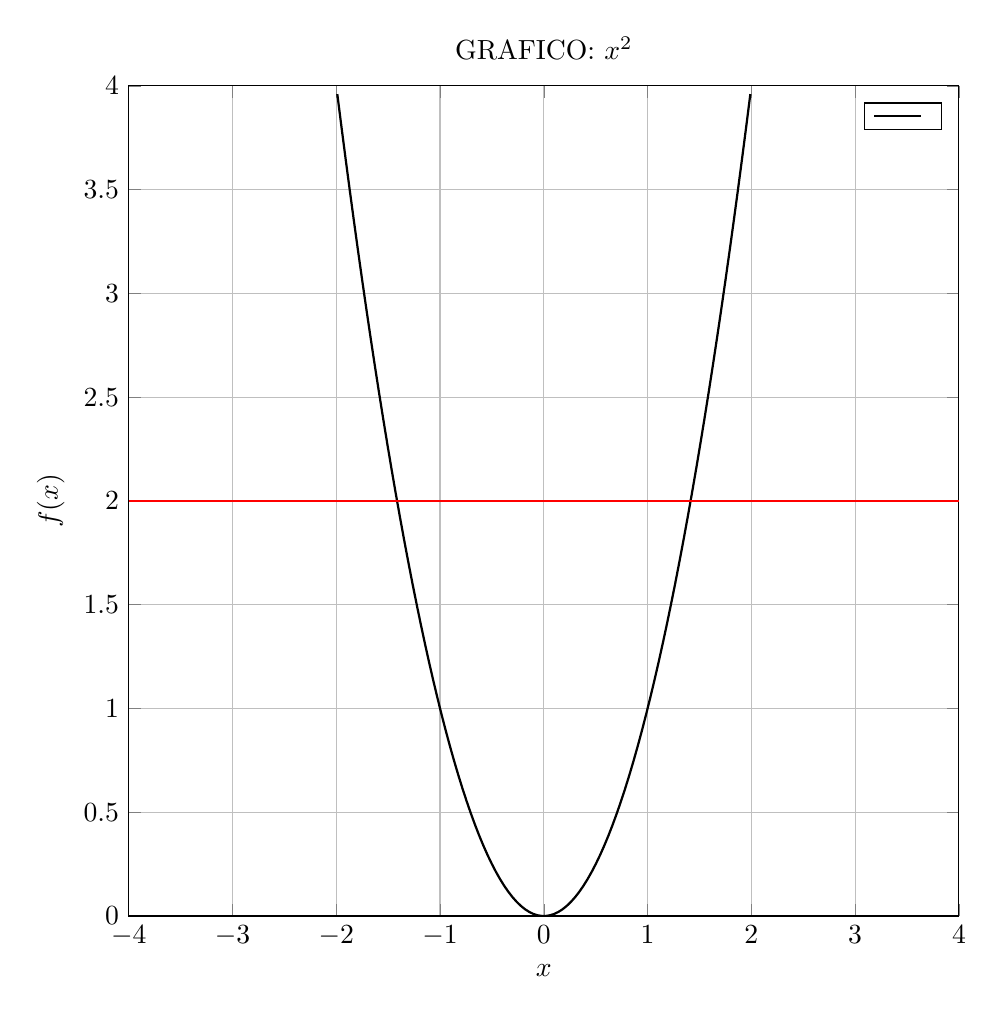
\begin{tikzpicture}
			\begin{axis}[
					title=GRAFICO: $x^{2}$,
					xmin=-4, xmax=4,
					ymin=0,ymax=4,
					restrict y to domain = 0:4, domain=-4:4, width=\textwidth, height=\textwidth, grid=major, samples=200,  ylabel=$f(x)$, xlabel=$x$, legend entries={$ $}]
				\addplot[black, thick] {x^2};
				\addplot[red, thick] {2};
			\end{axis}
		\end{tikzpicture}
	\end{center}
	\begin{itemize}
		\item Non è iniettiva
		\item Non è surgettiva
	\end{itemize}

\end{minipage}
%
\begin{minipage}[t]{0.48\textwidth}
	Esempio 2 $f : \R \rightarrow [0,\infty)$
	\begin{center}
		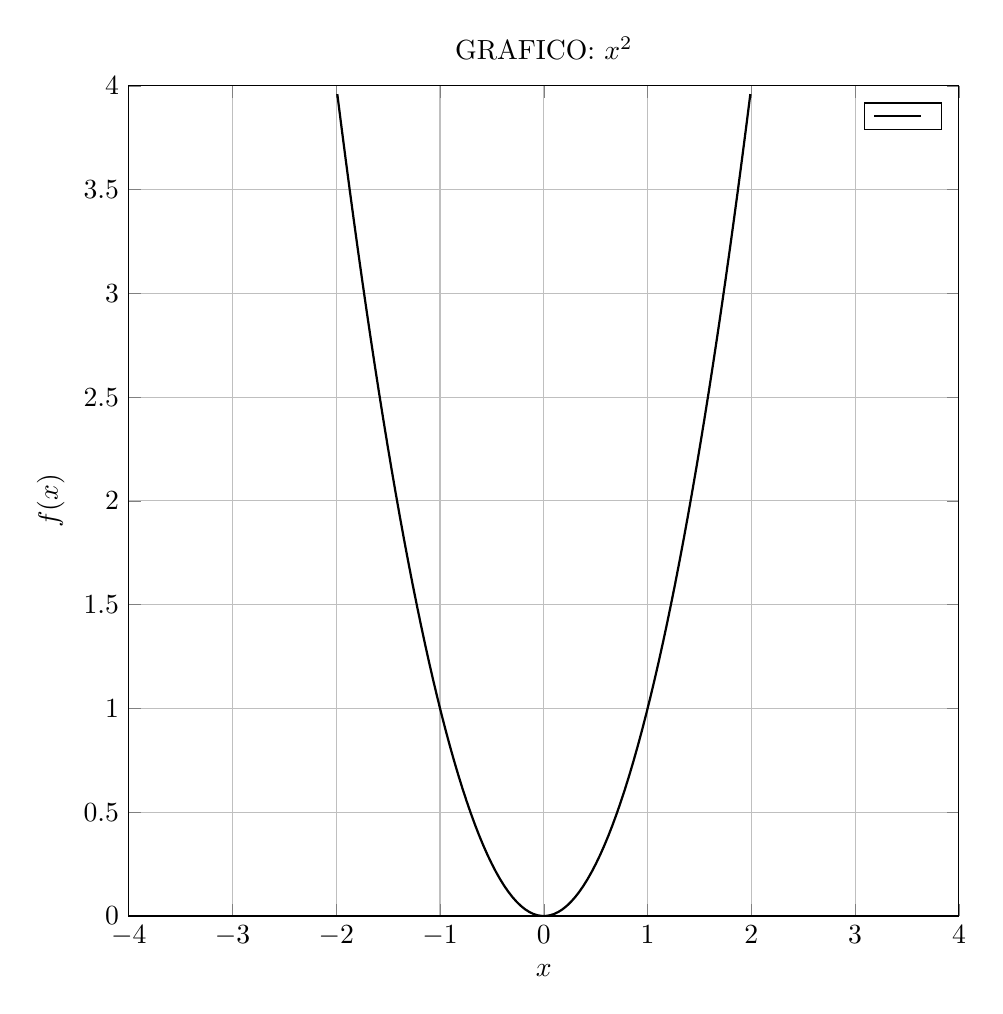
\begin{tikzpicture}
			\begin{axis}[
					title=GRAFICO: $x^2$,
					xmin=-4, xmax=4,
					ymin=0,ymax=4,
					restrict y to domain = 0:4, domain=-4:4, width=\textwidth, height=\textwidth, grid=major, samples=200,  ylabel=$f(x)$, xlabel=$x$, legend entries={$ $}]
				\addplot[black, thick] {x^2};
			\end{axis}
		\end{tikzpicture}
	\end{center}
	\begin{itemize}
		\item Non è iniettiva
		\item E' suriettiva
	\end{itemize}

\end{minipage}
\vskip1cm
\begin{minipage}[t]{0.48\textwidth}
	Esempio 3: $f : [0, \infty) \rightarrow \R$
	\begin{center}
		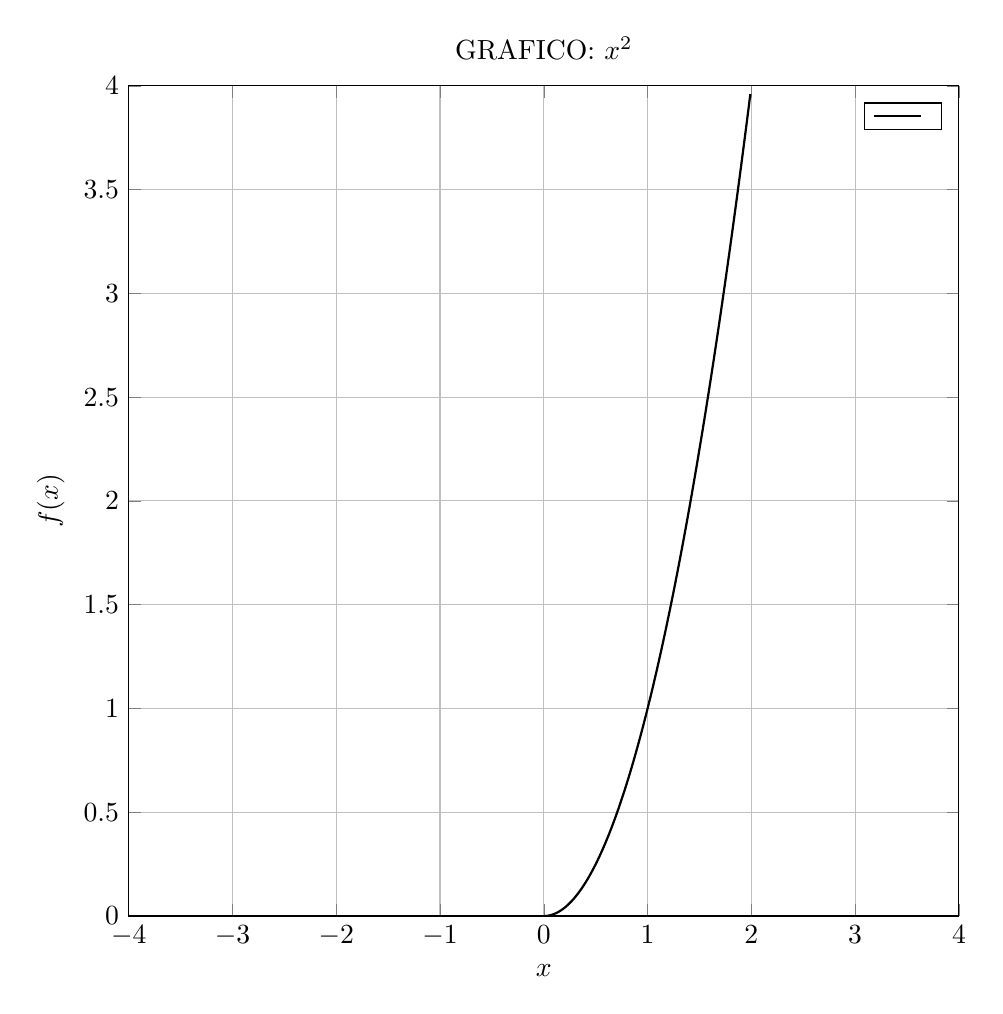
\begin{tikzpicture}
			\begin{axis}[
					title=GRAFICO: $x^2$,
					xmin=-4, xmax=4,
					ymin=0,ymax=4,
					restrict y to domain = 0:4, domain=0:4, width=\textwidth, height=\textwidth, grid=major, samples=200,  ylabel=$f(x)$, xlabel=$x$, legend entries={$ $}]
				\addplot[black, thick] {x^2};
			\end{axis}
		\end{tikzpicture}
	\end{center}
	\begin{itemize}
		\item E' iniettiva
		\item Non è surgettiva
	\end{itemize}

\end{minipage}
%
\begin{minipage}[t]{0.48\textwidth}
	Esempio 3: $f : [0, \infty) \rightarrow [0,\infty)$
	\begin{center}
		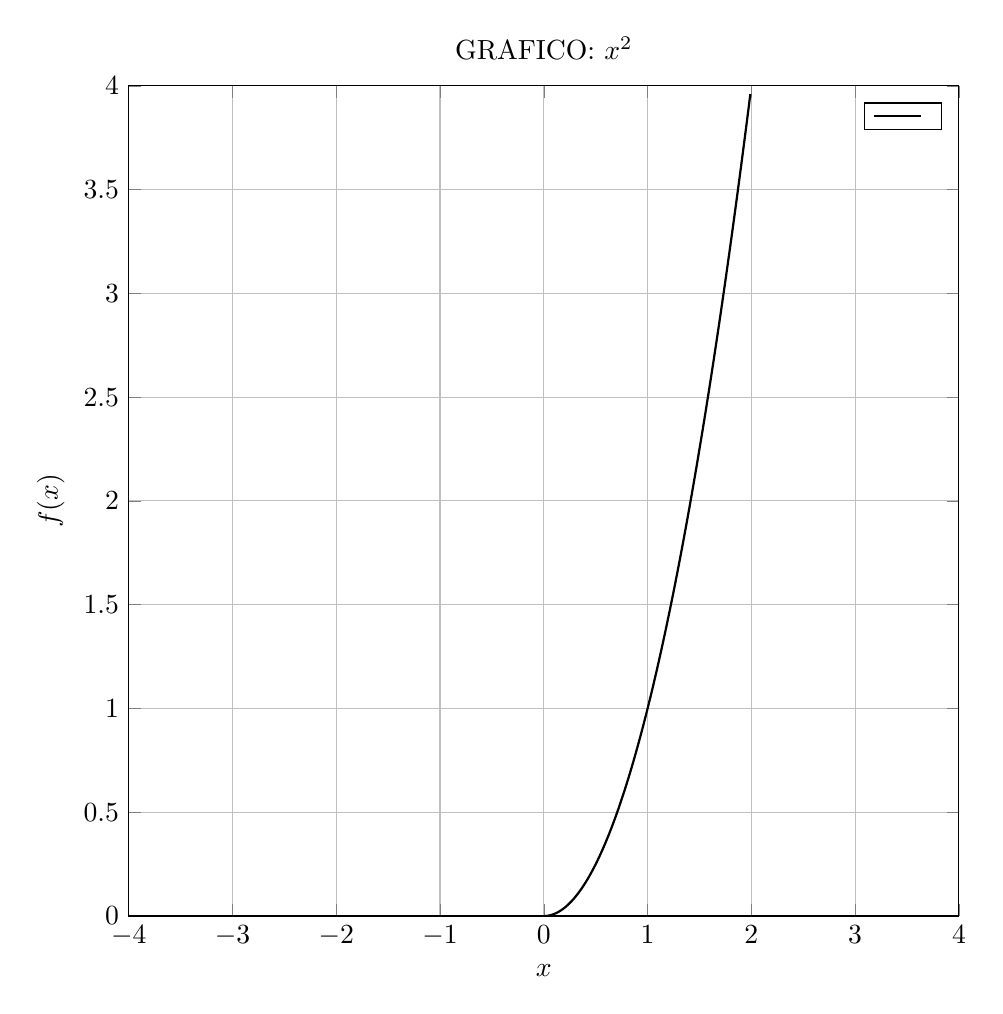
\begin{tikzpicture}
			\begin{axis}[
					title=GRAFICO: $x^2$,
					xmin=-4, xmax=4,
					ymin=0,ymax=4,
					restrict y to domain = 0:4, domain=0:4, width=\textwidth, height=\textwidth, grid=major, samples=200,  ylabel=$f(x)$, xlabel=$x$, legend entries={$ $}]
				\addplot[black, thick] {x^2};
			\end{axis}
		\end{tikzpicture}
	\end{center}
	\begin{itemize}
		\item E' iniettiva
		\item E' surgettiva
	\end{itemize}

\end{minipage}
\subsection{Operazioni sui grafici}
\begin{itemize}
	\item $ f\left( x \right) \to f\left( x \right) +x$ \quad traslazione in verticale (se c è positivo verso l'alto)
	\item $ f\left( x \right) \rightarrow f\left( x+c \right) $ \quad traslazione in orizzontale (se c è positivo verso sinistra)
	\item $f\left( x \right)  \rightarrow -f\left( x \right) $ \quad diventa speculare rispetto ad asse x
	\item $f\left( x \right) \rightarrow f\left( -x \right) $ diventa speculare rispetto all'asse y
	\item $f\left( x \right) \rightarrow \left|f\left( x \right) \right|$ \quad ogni parte negativa diventa ribaltata verso l'alto
	\item $f\left( x \right) \rightarrow f\left( \left|x\right| \right) $ \quad la parte del grafico con $x\ge 0 $ viene riflessa rispetto all'asse y
\end{itemize}
\begin{minipage}[t]{0.48\textwidth}
	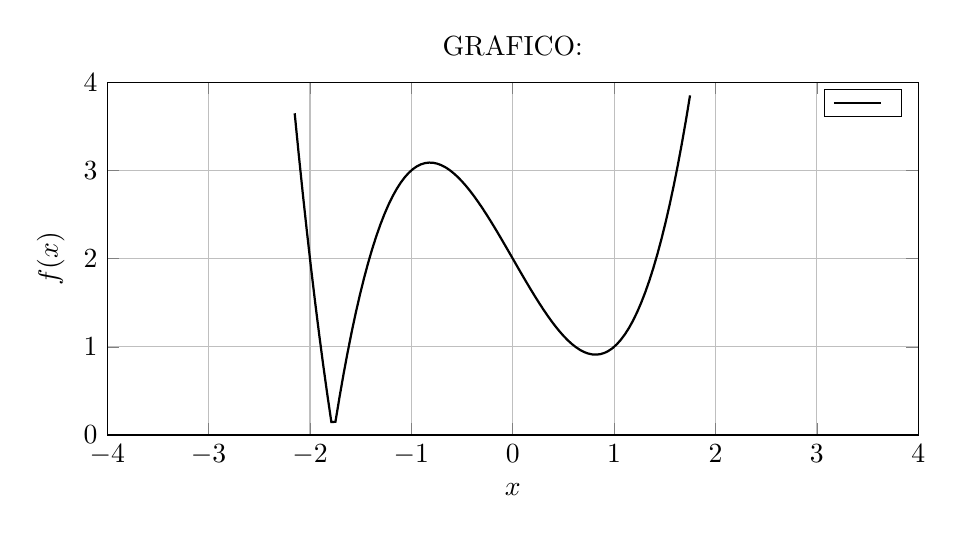
\begin{tikzpicture}
		\begin{axis}[title=GRAFICO: ,
				xmin=-4, xmax=4,
				ymin=0,ymax=4,
				restrict y to domain = 0:4, domain=-4:4, width=0.98\textwidth, height=0.5\textwidth, grid=major, samples=200,  ylabel=$f(x)$, xlabel=$x$, legend entries={$ $}]
			\addplot[black, thick] {abs(x^3-2*x+2)};
		\end{axis}
	\end{tikzpicture}
\end{minipage}
%
\begin{minipage}[t]{0.48\textwidth}

\end{minipage}

\subsection{Risoluzione di equazioni per via grafica}
Esempio 1: \[
	\left|\left|x\right|-1\right|=\frac{1}{2}
\]
\begin{minipage}[t]{0.48\textwidth}
	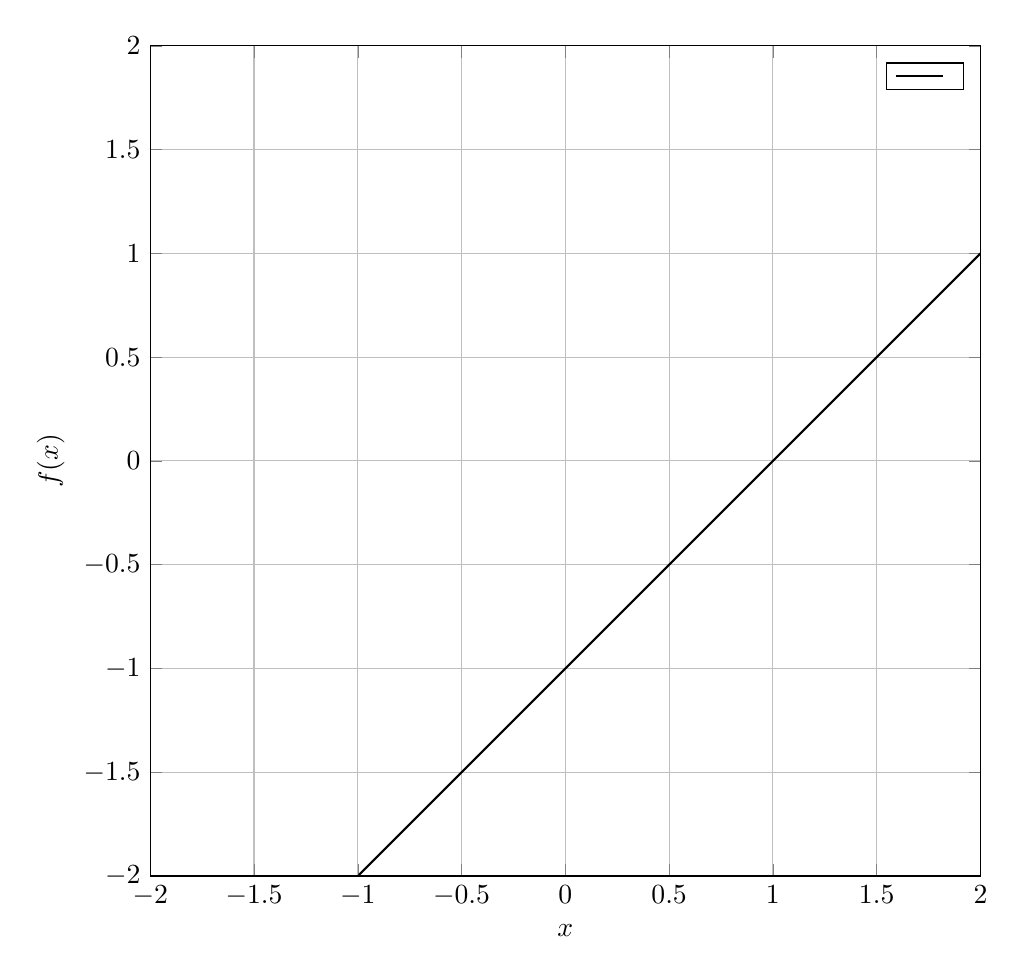
\begin{tikzpicture}
		\begin{axis}[
				xmin=-2, xmax=2,
				ymin=-2,ymax=2,
				restrict y to domain = -2:2, domain=-2:2, width=\textwidth, height=\textwidth, grid=major, samples=200,  ylabel=$f(x)$, xlabel=$x$, legend entries={$ $}]
			\addplot[black, thick] {x-1};
		\end{axis}
	\end{tikzpicture}
\end{minipage}
%
\begin{minipage}[t]{0.48\textwidth}
	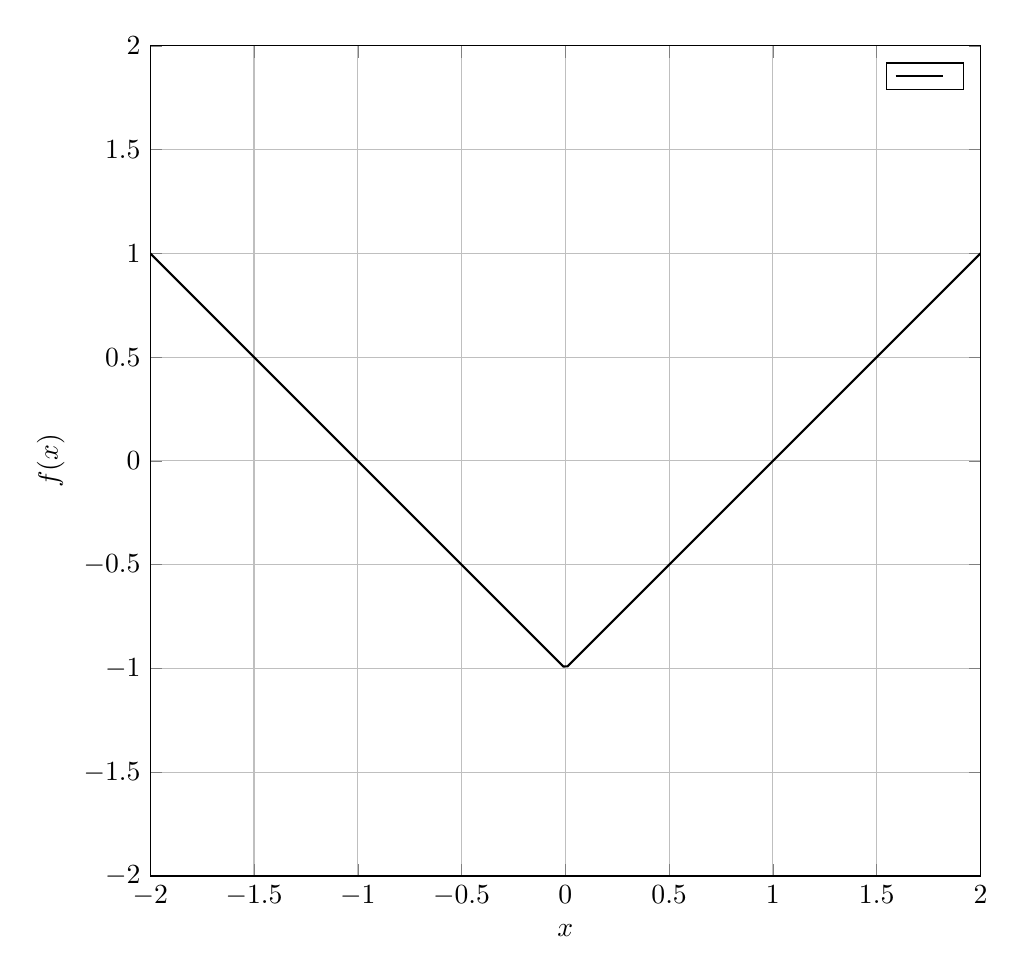
\begin{tikzpicture}
		\begin{axis}[
				xmin=-2, xmax=2,
				ymin=-2,ymax=2,
				restrict y to domain = -2:2, domain=-2:2, width=\textwidth, height=\textwidth, grid=major, samples=200,  ylabel=$f(x)$, xlabel=$x$, legend entries={$ $}]
			\addplot[black, thick] {abs(x)-1};
		\end{axis}
	\end{tikzpicture}
\end{minipage}
\begin{center}
	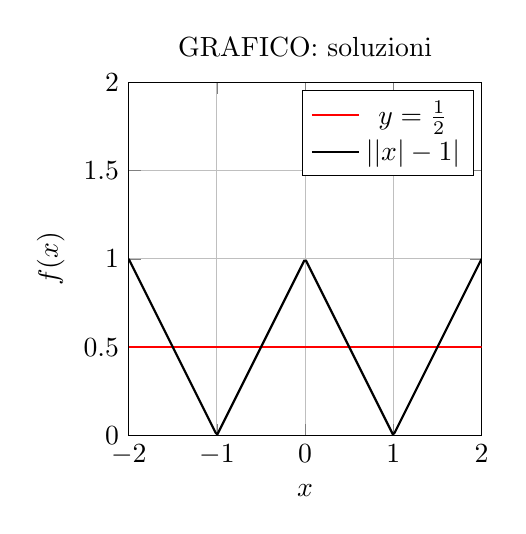
\begin{tikzpicture}
		\begin{axis}[
				title=GRAFICO: soluzioni ,
				xmin=-2, xmax=2,
				ymin=0,ymax=2,
				restrict y to domain = -2:2, domain=-2:2, width=0.5\textwidth, height=0.5\textwidth, grid=major, samples=200,  ylabel=$f(x)$, xlabel=$x$, legend entries={$y=\frac{1}{2}$, $ \left|\left|x\right|-1\right|$}]
			\addplot[red, thick] {0.5};
			\addplot[black, thick] {abs(abs(x)-1)};
		\end{axis}
	\end{tikzpicture}
\end{center}
Esercizio: determinare al variare di
$\lambda  \in  \R$ quali sono le soluzioni dell'equazione \[
	\left|\left( x+3 \right) ^3 -2\right|=\lambda
\]
\section{Potenze, esponenziali, funzioni trigonometriche}
\subsection{Potenze pari}


\begin{minipage}[t]{0.48\textwidth}
	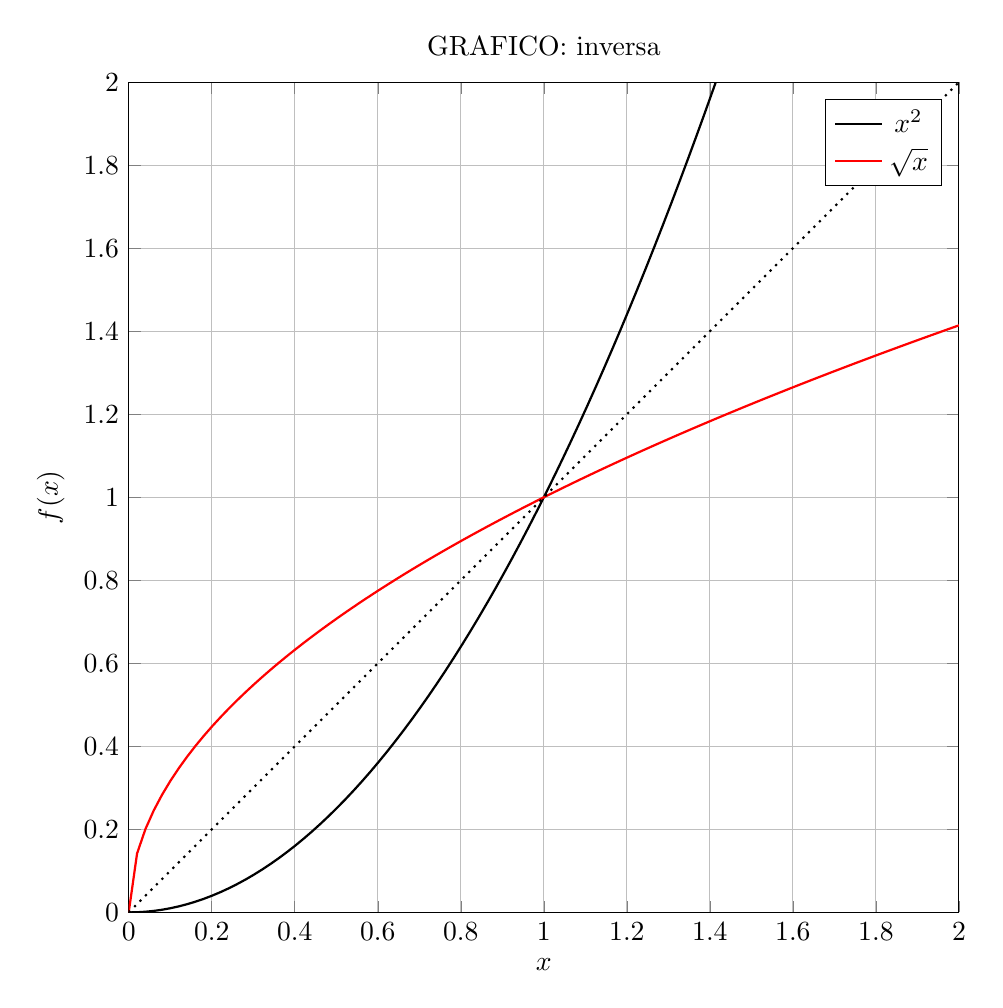
\begin{tikzpicture}
		\begin{axis}[
				title=GRAFICO: inversa,
				xmin=0, xmax=2,
				ymin=0,ymax=2,
				restrict y to domain = 0:4, domain=0:4, width=\textwidth, height=\textwidth, grid=major, samples=200,  ylabel=$f(x)$, xlabel=$x$, legend entries={$ x^2$, $\sqrt{x} $}]
			\addplot[black, thick] {x^2};
			\addplot[red, thick] {sqrt(x)};
			\addplot[dotted, thick] {x};
		\end{axis}
	\end{tikzpicture}
\end{minipage}
%
\begin{minipage}[t]{0.48\textwidth}
	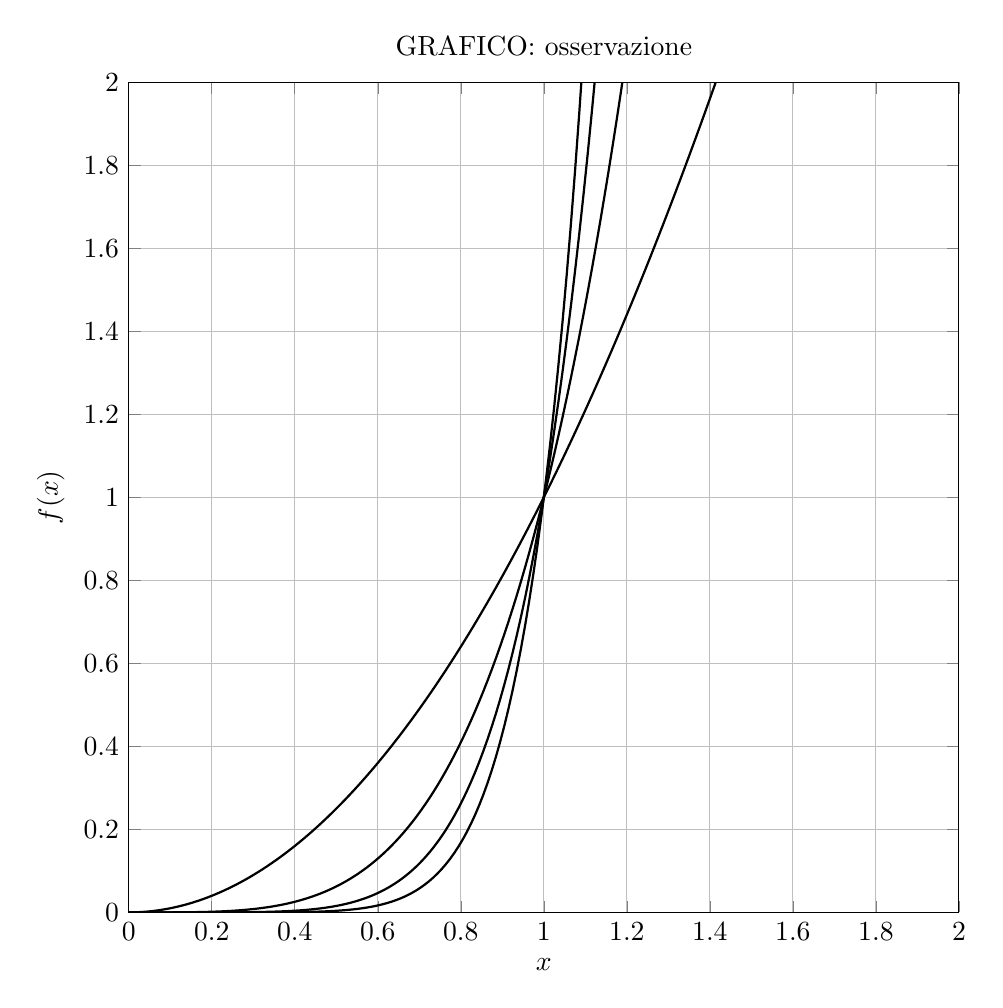
\begin{tikzpicture}
		\begin{axis}[
				title=GRAFICO: osservazione,
				xmin=0, xmax=2,
				ymin=0,ymax=2,
				restrict y to domain = 0:3, domain=0:2, width=\textwidth, height=\textwidth, grid=major, samples=200,  ylabel=$f(x)$, xlabel=$x$]
			\addplot[black, thick] {x^2};
			\addplot[black, thick] {x^4};
			\addplot[black, thick] {x^6};
			\addplot[black, thick] {x^8};
		\end{axis}
	\end{tikzpicture}
\end{minipage}

\subsection{Potenze dispari}
\begin{center}
	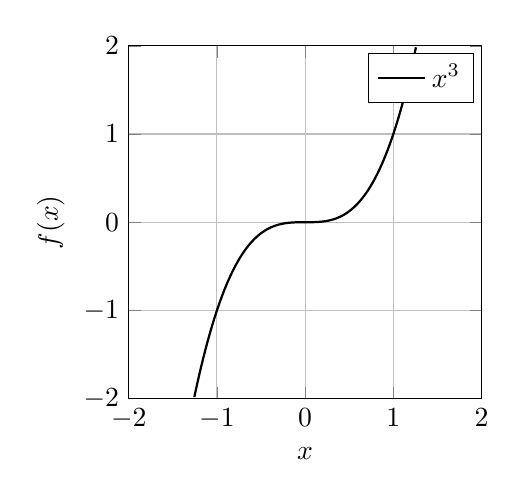
\begin{tikzpicture}
		\begin{axis}[
				xmin=-2, xmax=2,
				ymin=-2,ymax=2,
				restrict y to domain = -2:2, domain=-2:2, width=0.5\textwidth, height=0.5\textwidth, grid=major, samples=200,  ylabel=$f(x)$, xlabel=$x$, legend entries={$ x^3 $}]
			\addplot[black, thick] {x^3};
		\end{axis}
	\end{tikzpicture}
\end{center}

\textbox{OSS: se una funzione $f\left( x \right) $ è iniettiva e $a = b$ allora $f\left( a \right) = f\left( b \right) $. Se $ a > b$ allora $f\left( x \right) > f\left( b \right) $ se $f$ è crescente}
\subsection{Esponenziale e logaritmo}
\begin{minipage}[t]{0.48\textwidth}
	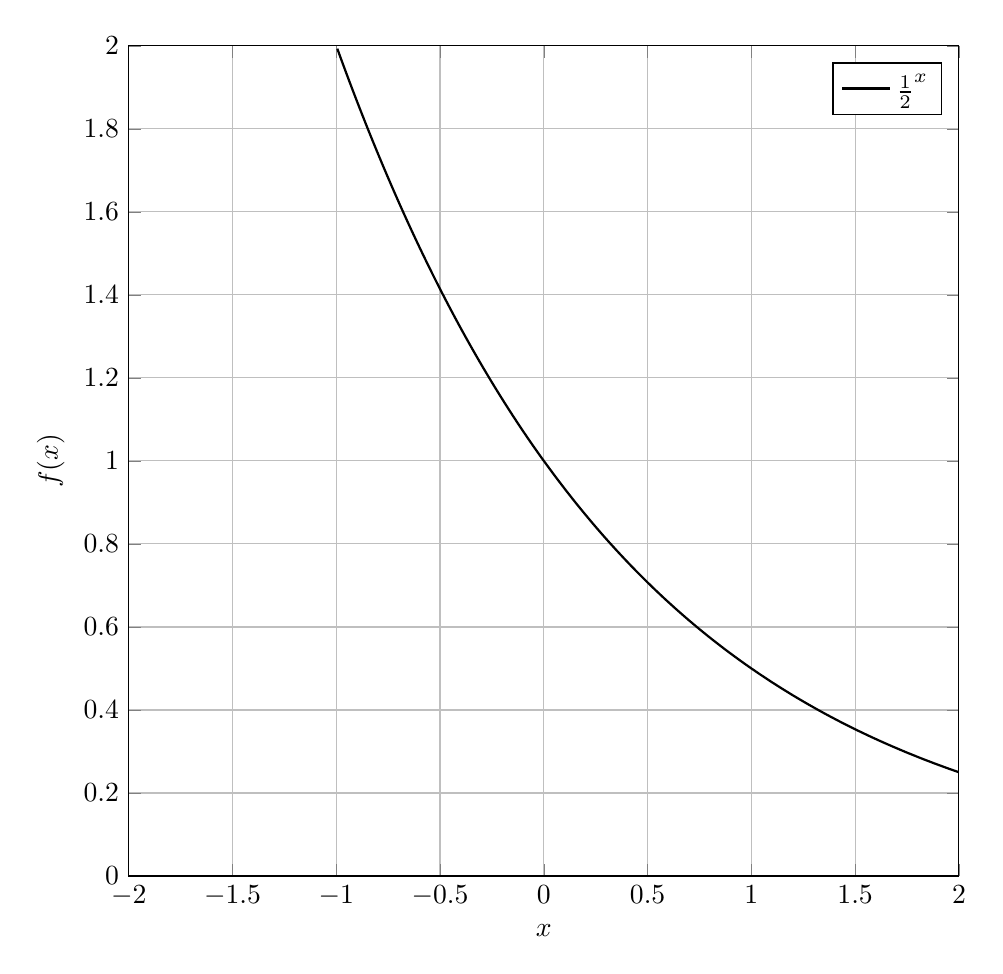
\begin{tikzpicture}
		\begin{axis}[
				xmin=-2, xmax=2,
				ymin=0,ymax=2,
				restrict y to domain = -2:2, domain=-2:2, width=\textwidth, height=\textwidth, grid=major, samples=200,  ylabel=$f(x)$, xlabel=$x$, legend entries={$\frac{1}{2}^{x}$}]
			\addplot[black, thick] {0.5^x};
		\end{axis}
	\end{tikzpicture}
\end{minipage}
%
\begin{minipage}[t]{0.48\textwidth}
	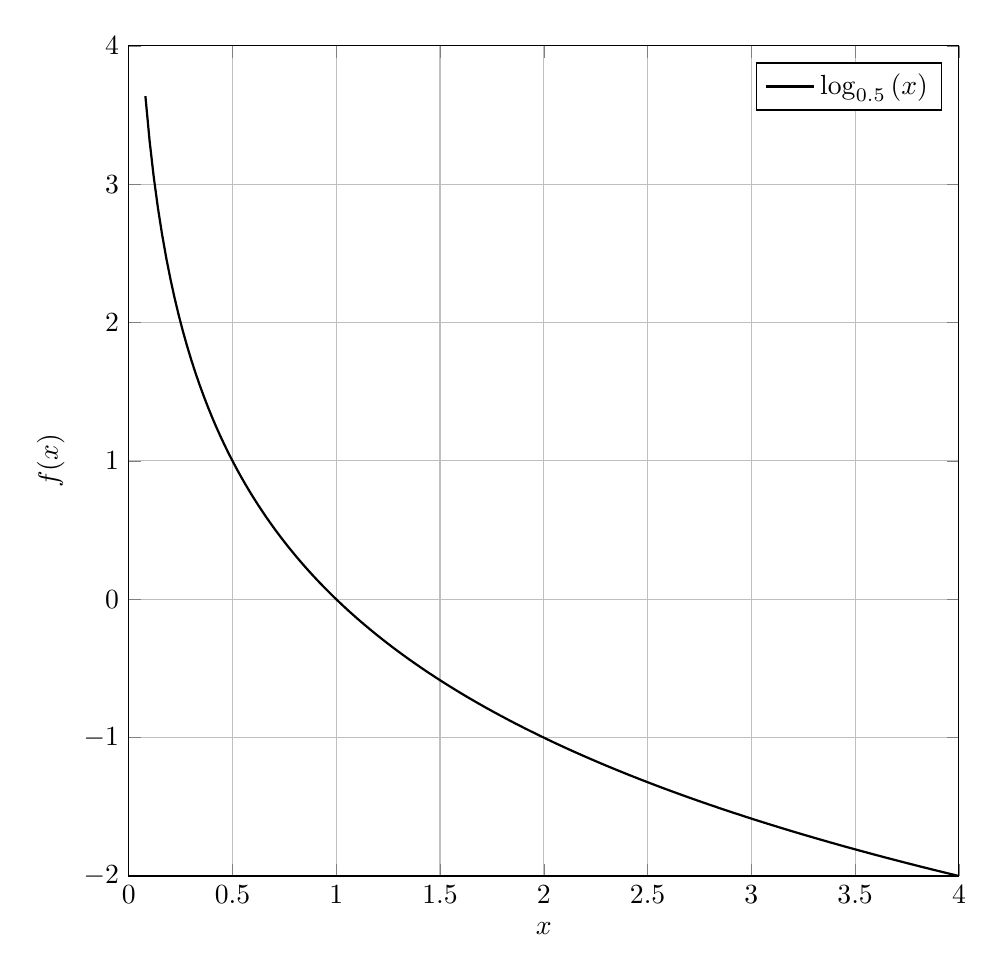
\begin{tikzpicture}
		\begin{axis}[
				xmin=0, xmax=4,
				ymin=-2,ymax=4,
				restrict y to domain = -2:4, domain=0:4, width=\textwidth, height=\textwidth, grid=major, samples=200,  ylabel=$f(x)$, xlabel=$x$, legend entries={$ \log_{0.5} \left( x \right) $}]
			\addplot[black, thick] {ln(x)/ln(0.5)};
		\end{axis}
	\end{tikzpicture}
\end{minipage}
\[
	e^{x} + e^{y} = e^{x+y} \quad \left( e^{x} \right) ^{y}= e^{xy}
\]

\subsection{Funzioni trigonometriche}
\begin{minipage}[t]{0.48\textwidth}
	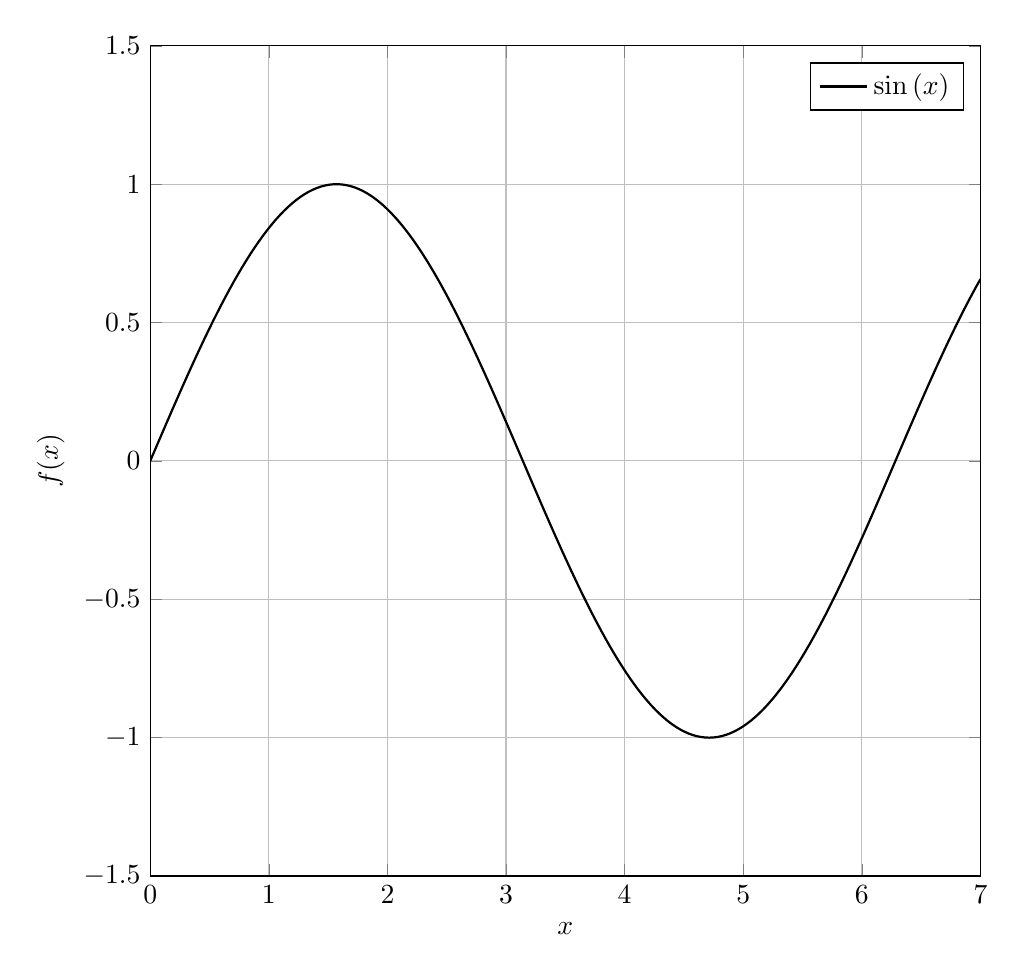
\begin{tikzpicture}
		\begin{axis}[
				xmin=0, xmax=7,
				ymin=-1.5,ymax=1.5,
				restrict y to domain =-2:2, domain=0:7, width=\textwidth, height=\textwidth, grid=major, samples=200,  ylabel=$f(x)$, xlabel=$x$, legend entries={$ \sin\left( x \right)  $}]
			\addplot[black, thick] {sin(deg(x))};
		\end{axis}
	\end{tikzpicture}
\end{minipage}
%
\begin{minipage}[t]{0.48\textwidth}
	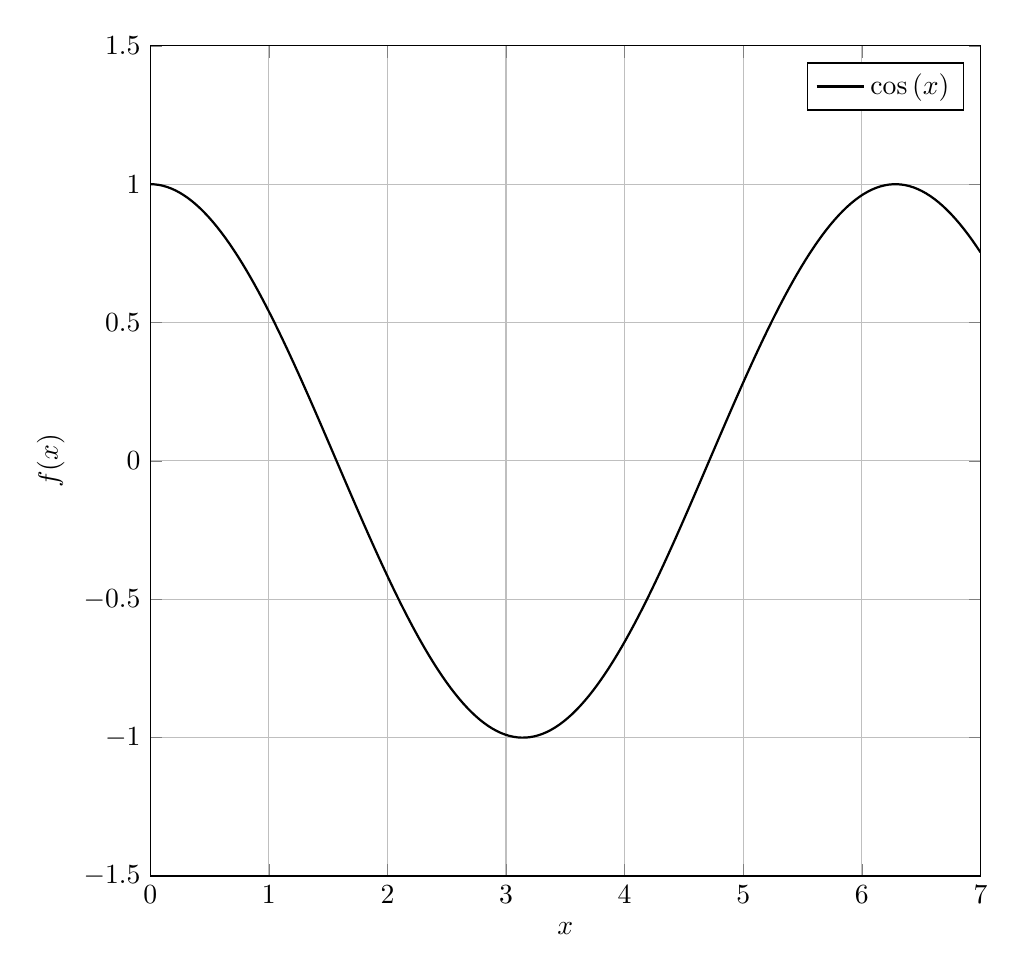
\begin{tikzpicture}
		\begin{axis}[
				xmin=0, xmax=7,
				ymin=-1.5,ymax=1.5,
				restrict y to domain =-2:2, domain=0:7, width=\textwidth, height=\textwidth, grid=major, samples=200,  ylabel=$f(x)$, xlabel=$x$, legend entries={$ \cos\left( x \right)  $}]
			\addplot[black, thick] {cos(deg(x))};
		\end{axis}
	\end{tikzpicture}
\end{minipage}

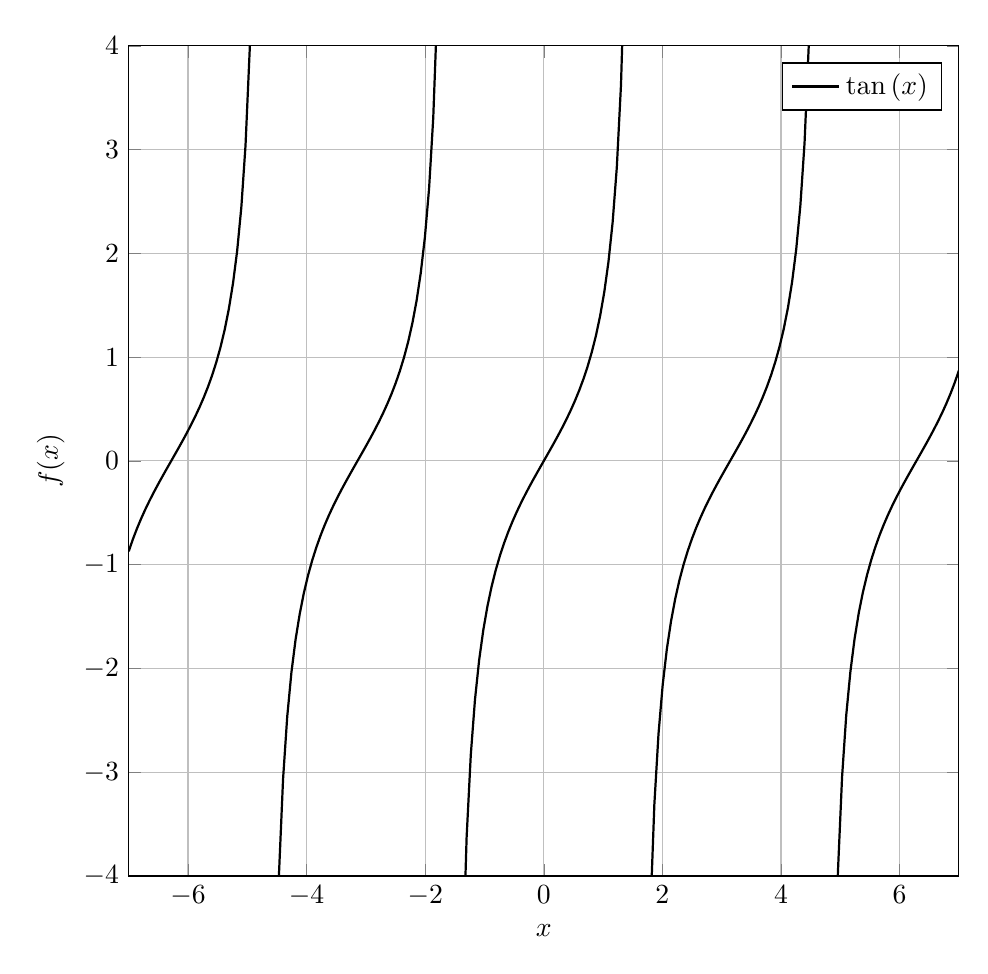
\begin{tikzpicture}
	\begin{axis}[
			xmin=-7, xmax=7,
			ymin=-4,ymax=4,
			restrict y to domain =-7:7, domain=-7:7, width=\textwidth, height=\textwidth, grid=major, samples=200,  ylabel=$f(x)$, xlabel=$x$, legend entries={$ \tan \left( x \right) $}]
		\addplot[black, thick] {tan(deg(x))};
	\end{axis}
\end{tikzpicture}
\subsubsection{Inverto il seno}
Il seno non è ne iniettivo ne surgettivo a meno che non lo consideri come:
\[
	f: \left[ -\frac{\pi}{2}, \frac{\pi}{2} \right] \rightarrow \left[ -1,1 \right]
\]
Il coseno non è ne iniettivo ne survettivo a meno che non lo si consideri come:
\[
	f: \left[ 0, \pi \right] \rightarrow \left[ -1,1 \right]
\]


\begin{minipage}[t]{0.48\textwidth}
	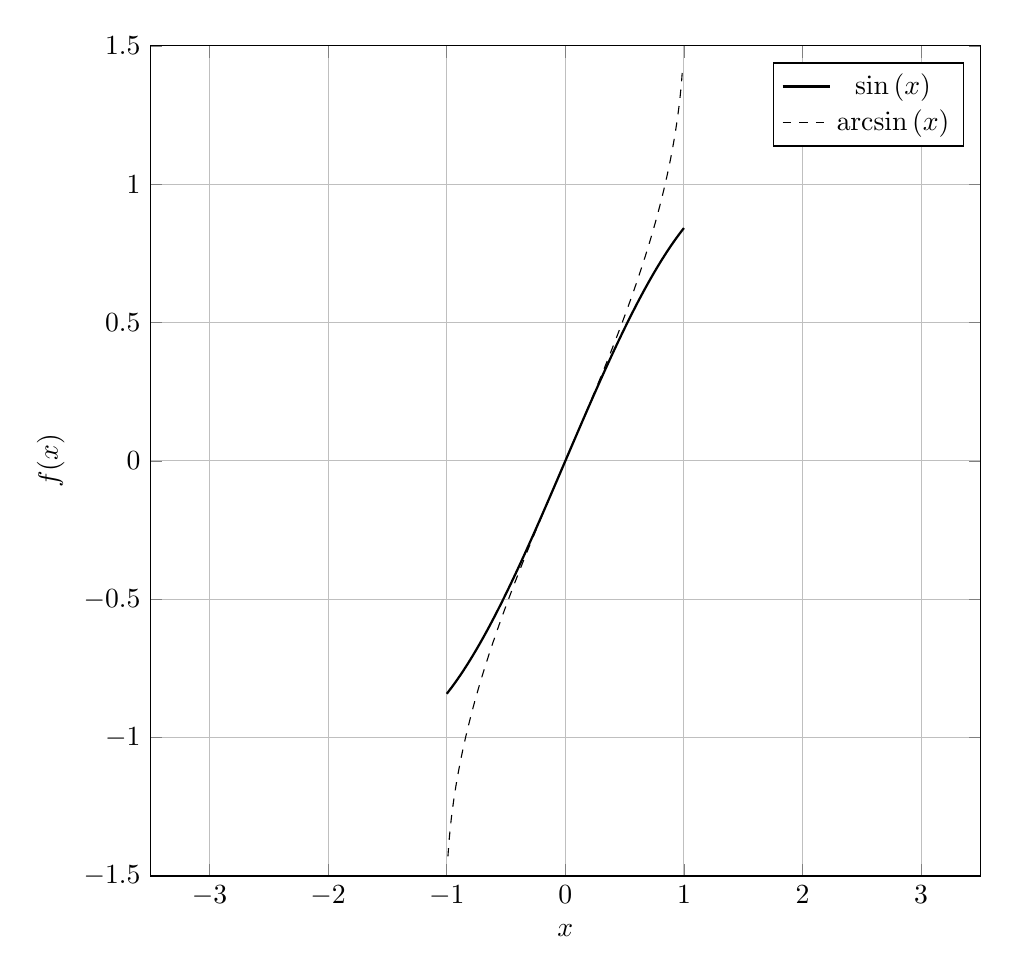
\begin{tikzpicture}
		\begin{axis}[
				xmin=-3.5, xmax=3.5,
				ymin=-1.5,ymax=1.5,
				restrict y to domain = -1.5:1.5, domain=-1:1, width=\textwidth, height=\textwidth, grid=major, samples=200,  ylabel=$f(x)$, xlabel=$x$, legend entries={$ \sin\left( x \right)  $, $ \arcsin \left( x \right)  $}]
			\addplot[black, thick] {sin(deg(x))};
			\addplot[dashed, domain=-1:1] {asin(x)/180*pi};
		\end{axis}
	\end{tikzpicture}
\end{minipage}
%
\begin{minipage}[t]{0.48\textwidth}
	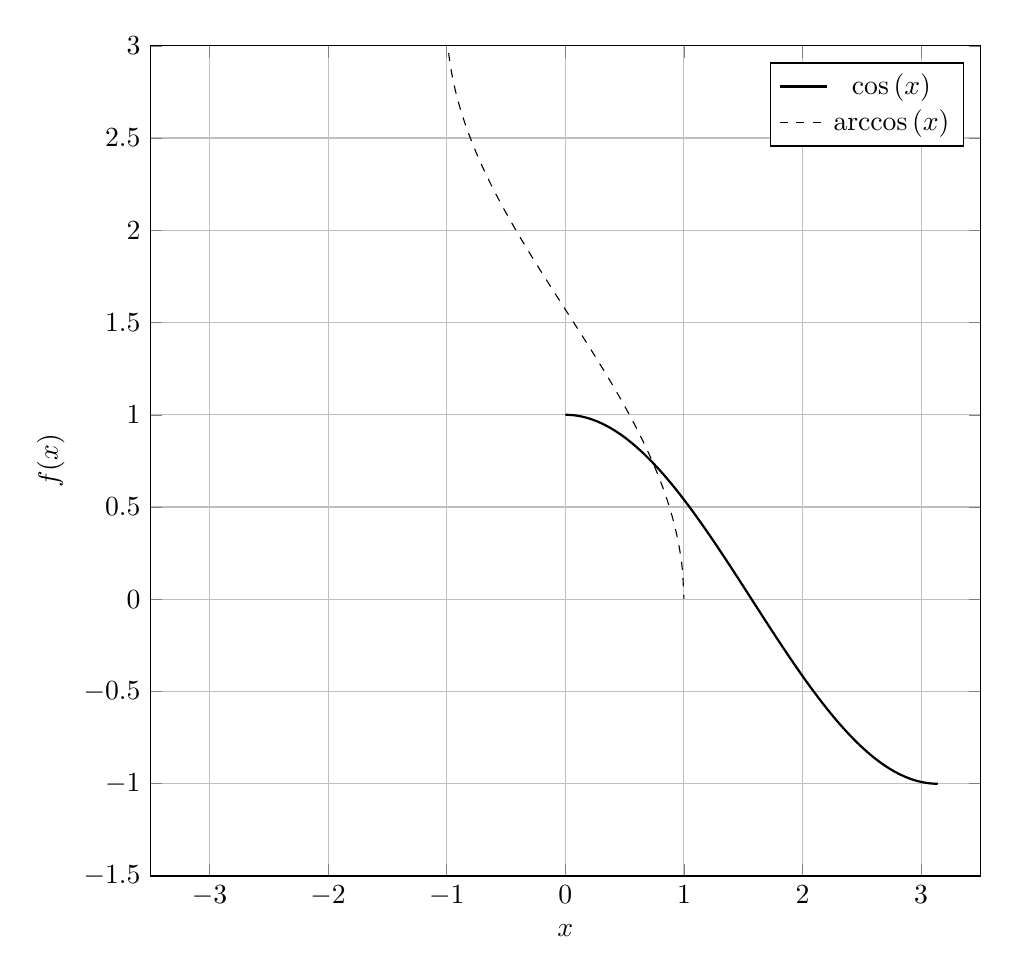
\begin{tikzpicture}
		\begin{axis}[
				xmin=-3.5, xmax=3.5,
				ymin=-1.5,ymax=3,
				restrict y to domain = -10:10, domain=0:3.14, width=\textwidth, height=\textwidth, grid=major, samples=200,  ylabel=$f(x)$, xlabel=$x$, legend entries={$ \cos \left( x \right) 	 $, $ \arccos \left( x \right) $}]
			\addplot[black, thick] {cos(deg(x))};
			\addplot[dashed, domain=-1:1] {acos(x)/180*pi};
		\end{axis}
	\end{tikzpicture}

\end{minipage}
\subsection{Funzioni iperboliche}
\[
	\cosh = \frac{e^{x} + e^{-x}}{2} \rightarrow pari
\]
\[
	\sinh = \frac{e^{x} - e^{-x}}{2} \rightarrow dispari
\]
\[
	\tanh = \frac{\sinh}{\cosh} \rightarrow dispari
\]
\begin{minipage}[t]{0.48\textwidth}
	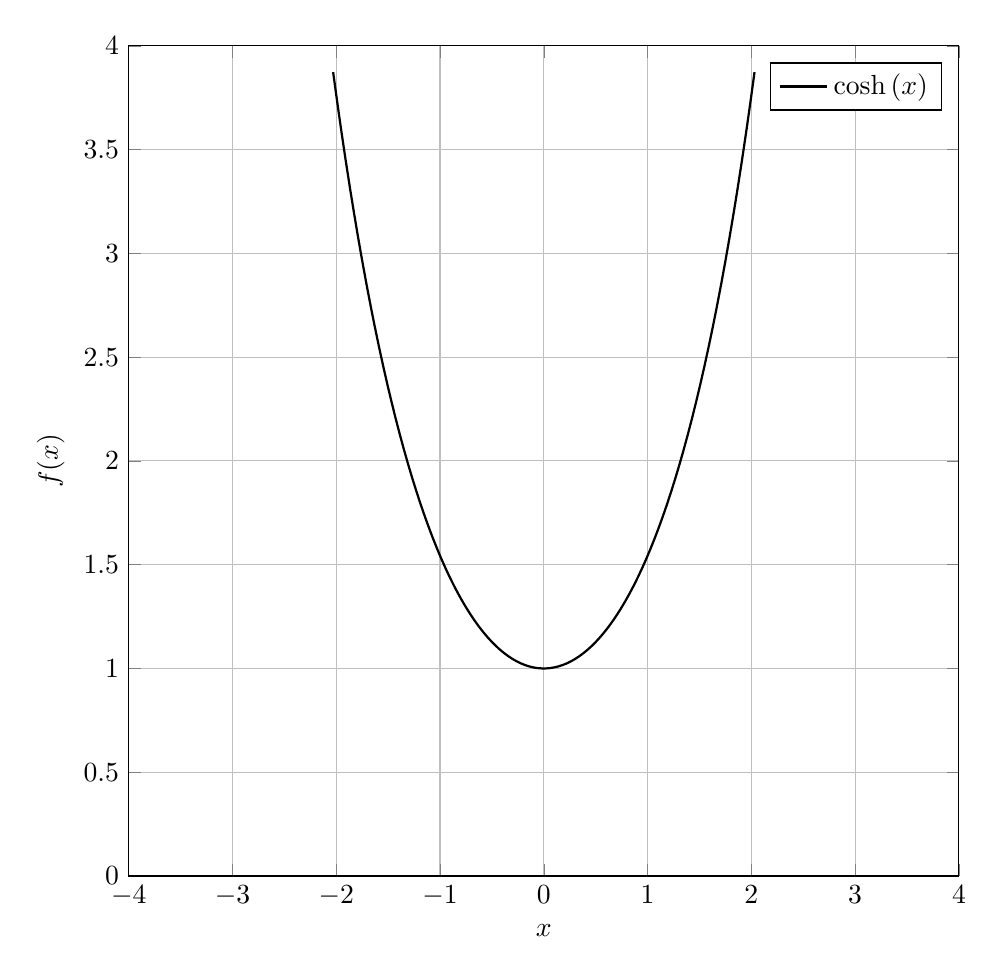
\begin{tikzpicture}
		\begin{axis}[
				xmin=-4, xmax=4,
				ymin=0,ymax=4,
				restrict y to domain = 0:4, domain=-4:4, width=\textwidth, height=\textwidth, grid=major, samples=200,  ylabel=$f(x)$, xlabel=$x$, legend entries={$ \cosh \left( x \right) $}]
			\addplot[black, thick] {cosh(x)};
		\end{axis}
	\end{tikzpicture}
\end{minipage}
%
\begin{minipage}[t]{0.48\textwidth}
	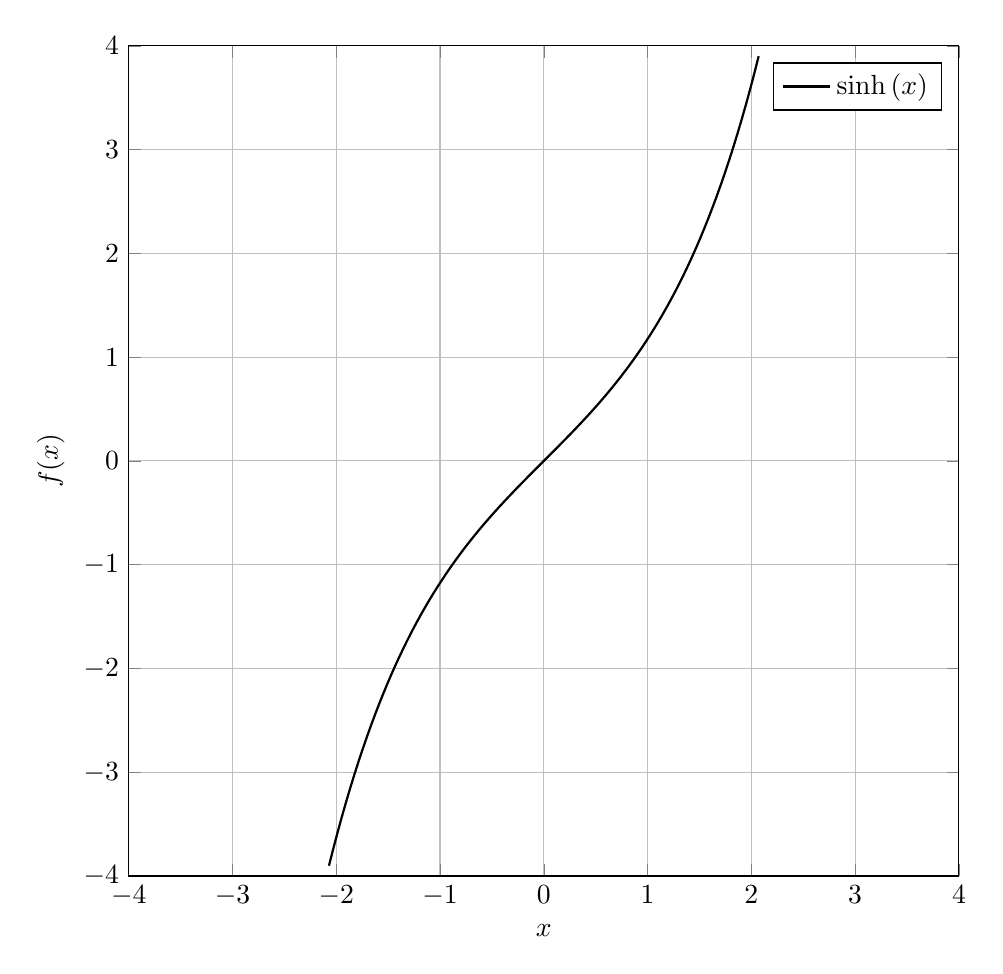
\begin{tikzpicture}
		\begin{axis}[
				xmin=-4, xmax=4,
				ymin=-4,ymax=4,
				restrict y to domain = -4:4, domain=-4:4, width=\textwidth, height=\textwidth, grid=major, samples=200,  ylabel=$f(x)$, xlabel=$x$, legend entries={$ \sinh \left( x \right) $}]
			\addplot[black, thick] {sinh(x)};
		\end{axis}
	\end{tikzpicture}
\end{minipage}

\begin{center}
	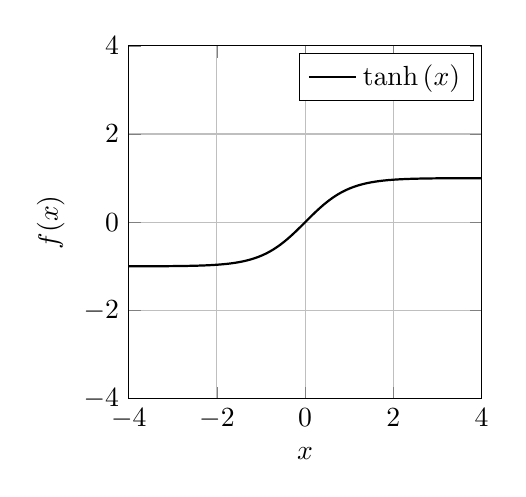
\begin{tikzpicture}
		\begin{axis}[
				xmin=-4, xmax=4,
				ymin=-4,ymax=4,
				restrict y to domain = -4:4, domain=-4:4, width=0.5\textwidth, height=0.5\textwidth, grid=major, samples=200,  ylabel=$f(x)$, xlabel=$x$, legend entries={$ \tanh \left( x \right)  $}]
			\addplot[black, thick] {tanh(x)};
		\end{axis}
	\end{tikzpicture}
\end{center}


\subsection{Formule trigonometria iperbolica}
\textbox{Queste formule sono molto simili alle formule della trigonometria tradizionale}
\[
	\sin\left( 2x \right) = 2 \sin \left( x \right) \cos\left( x \right)
\]
\[
	\sinh \left( 2x \right)  = \frac{e^{2x} - e ^{-2x}}{2} = \frac{\left( e^{x} \right) ^{2} - \left( e^{-x} \right) ^{2}}{2}= \frac{\left( e^{x}- e^{-x} \right)  \left( e^{x} + e^{-x} \right)}{2} = 2 \sinh\left( x \right) \cosh \left( x \right)
\]
Formula fondamentale della trigonometria \[
	\sinh ^2 x = \left( \frac{e^{x} - e ^{ -x}}{2} \right) ^2 = \frac{e^{2} + e^{2x}- 2}{4}
\]
\[
	\cosh ^2 x = \left( \frac{e^{x} + e ^{ -x}}{2} \right) ^2 = \frac{e^{2} + e^{2x}+ 2}{4}
\]
\[
	\cosh ^2x - \sinh ^2 x = 1
\]
\section{Esercizi}
\subsection{Esercizio 1}

\teorema{Insiemi limitati}{Se un insieme $S \neq \emptyset$ è \underline{limitato superiormente/inferiormente} esso ammette \underline{estremo superiore/inferiore}}
\label{teo6}
\bigbox{
	Dato un un insieme $S$ limitato inferiormente ma non superiormente e un insieme $L$ costituito da tutti i minoranti di $S$ allora \[
		\text{sup}L \text{ esiste e sup}L= \text{ inf}A
	\]
}
\begin{itemize}
	\item L'insieme $S$ denota tutti i maggioranti di $L$
	      \[
		      y \ge x \quad \forall y  \in S, x  \in L
	      \]
	\item Vito che $L$ ammette maggioranti, esso è limitato superiormente e per il teorema \ref{teo6} ammette estremo superiore sup$L$=$\beta$
	\item Visto che l'insieme $S$ denota i maggioranti di $L$, allora \[
		      \text{ se } x < \beta \rightarrow \text{ x non è maggiorante } \rightarrow x  \not\in S
	      \]
	      al contrario, tuttavia
	      \[
		      \text{ se } x  \in S \rightarrow x \ge \beta \rightarrow \beta\text{ è minorante di } S
	      \]
	\item Se prendo $\epsilon > \beta$ so che questa non appartiene a $L $ in quanto è più grande di un suo maggiorante, dunque \[
		      \text{ se  } \epsilon > \beta \rightarrow \epsilon  \not\in L \rightarrow \text{ non è minorante di S }
	      \]
	\item Dunque $\beta$:
	      \begin{enumerate}
		      \item E minorante di S
		      \item Se $\epsilon > \beta \rightarrow \epsilon \text{ non è minorante di } S$
	      \end{enumerate}
	      \bigbox{ $\beta $ è dunque \underline{estremo inferiore di $S$}\[
			      \text{ supL}= \text{ infS }=\beta
		      \] }
\end{itemize}
\subsection{Esercizio 2}
Dato l'insieme
\[
	A = \left\{ a_n = \frac{\cos \left( \pi n  \right)}{n^2 + 1}, \quad n  \in \N  \right\}
\]
si determini limite superiore, inferiore, massimo e minimo se presenti.
\begin{itemize}
	\item Scrivo qualche termine  \[
		      a_0 = 1 , a_1 = -\frac{1}{2}, a_2= \frac{1}{5}, a_3 = -\frac{1}{10}, a_4=\frac{1}{17}
	      \]
	\item Osservo che \[
		      \left|a_n\right|> \left|a_n+1\right| \quad \forall n  \in  \N
	      \]
	\item $\left|a_n\right| = \left| \frac{\cos \left( \pi n \right) }{n^2 +1}\right|= \frac{1}{n^2 + 1}$ in quanto $\cos\left( \pi n \right) $ è sempre uguale a $\pm 1$
	\item Risolvo disequazione \rarr è vera $ \forall n  \in  \N$
	      \[
		      \frac{1}{n^2 +1} \ge \frac{1}{\left( n+1 \right) ^2 + 1}
	      \]
	\item Visto che la successione decresce in valore assoluto posso affermare che
\end{itemize}

\begin{table}[h!]
	\centering
	\begin{tabular}{|ll|}
		\hline
		Estremo superiore & 1              \\
		Estremo inferiore & $-\frac{1}{2}$ \\
		Massimo           & 1              \\
		Minimo            & $-\frac{1}{2}$ \\
		\hline
	\end{tabular}
\end{table}
\subsection{Esercizio 3}
Dato l'insieme
\[
	A = \left\{ a_n = \frac{N^2 - 5}{n^2 +2}, \quad  n  \in  \N \right\}
\]

si determini limite superiore, inferiore, massimo e minimo se presenti.
\begin{itemize}
	\item Scrivo qualche termine
	      \[
		      a_0 = \frac{5}{2}, a_1 = - \frac{4}{3} , a-2 = -\frac{1}{6}, a_3 =\frac{4}{11}
	      \]
	\item Noto che termini sono crescenti e lo verifico risolvendo la disequazione: \[
		      \frac{\left( n+1 \right) ^2 -5}{\left( n+1 \right) ^2 + 2} > \frac{n^2 -5 }{n^2 +2}
	      \]
	      \[
		      \frac{14n + 7}{\left( n^2 + 2 \right) \left( \left( n+1 \right) ^2 +2  \right) } > 0 \quad \forall n  \in  \N
	      \]
	\item Noto che $\lim_{n \to \infty} \frac{n^2 -5}{n^2 + 2} = 1 $ dunque è probabile che 1 costituisca l'estremo superiore. Verifico che ciò è vero nel seguente modo:
	      \begin{itemize}
		      \item Ricordo definizione estremo: $\beta$ è estremo superiore se:
		            \[
			            \forall \varepsilon > 0 \quad  \exists x  \in A \text{ t.c. } x > \beta - \varepsilon
		            \]
		      \item Se la disequazione seguente ha soluzione per almeno un $n  \in  \N$, allora vuol dire che esiste un $ n  \in  A \text{ t.c. } a_n > \beta - \varepsilon$
		            \[
			            1-\varepsilon < \frac{n^2 -5}{n^2 + 2}
		            \]
		            \[
			            n > \left( \text{ int } \right) \sqrt{\frac{7}{\varepsilon}-2} +1
		            \]
		      \item La disequazione ha soluzioni per ogni valore positivo di $\varepsilon$ e  $\beta $ è un \underline{estremo superiore}
	      \end{itemize}
\end{itemize}
\begin{table}[h!]
	\centering
	\begin{tabular}{|ll|}
		\hline
		Estremo superiore & 1              \\
		Estremo inferiore & $-\frac{5}{2}$ \\
		Massimo           & no             \\
		Minimo            & $-\frac{5}{2}$ \\
		\hline
	\end{tabular}
\end{table}
\section{Numeri complessi}
\subsection{Forma cartesiana}
\bigbox{Un numero completto è un oggetto del tipo \[
	\underbrace{a}_{\text{Parte reale}} + \underbrace{b}_{\text{Parte immaginaria}}i
\]
dove $a$ e $b$ sono numeri reali e $i$ è un numero tale che $i^2= -1$}
\begin{minipage}[t]{0.48\textwidth}
	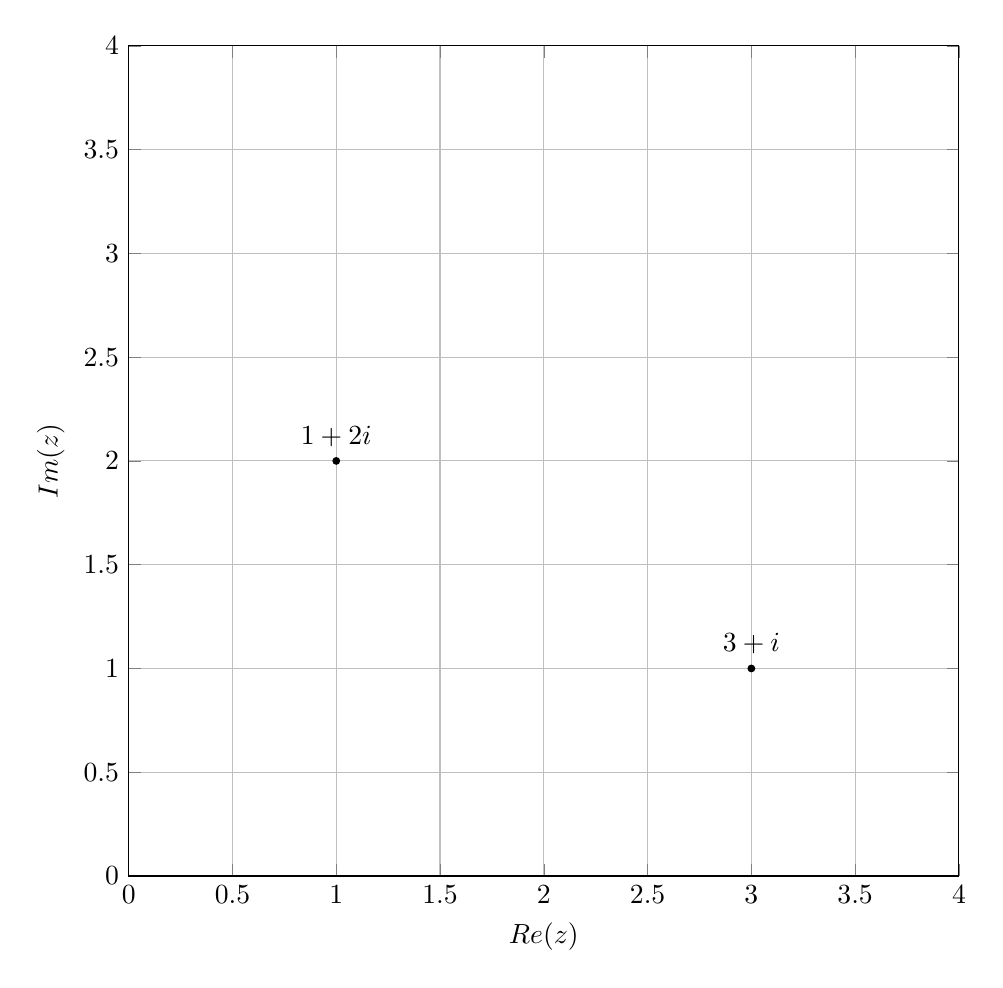
\begin{tikzpicture}
		\begin{axis}[
				xmin=0,xmax=4,
				ymin=0,ymax=4,
				restrict y to domain = 0:4, domain=0:4, width=\textwidth, height=\textwidth, grid=major, samples=200,  ylabel=$Im(z)$, xlabel=$Re(z)$]
			\node [circle, fill= black, inner sep=1, label= $1+2i$] at (1,2){};
			\node [circle, fill= black, inner sep=1, label= $3 + i$] at (3,1){};
		\end{axis}
	\end{tikzpicture}
\end{minipage}
%
\begin{minipage}[t]{0.48\textwidth}
	\begin{itemize}
		\item L'asse y è detta asse immaginaria
		\item Un numero con parte i mmaginaria nulla è detto puro
	\end{itemize}
\end{minipage}

\subsection{Somme e differenze}
\bigbox{Dati $z= a+bi, \quad w = c + di \quad  \in \C$ la loro somma è data da:
	\[
		\left( a+c \right) + \left( b+d \right) i
	\] }
\subsection{Prodotto}
\bigbox{Si usa la proprietà distributiva per il fatto che $i^2 = -1$ \[
		z * w = \left( a + bi \right) \left( c + di \right) = ac + adi + bci + bd \underbrace{i^2}_{=-1}
	\] }
\subsection{Reciproco}
\bigbox{Dato un numero $ z  \in  \C$, al fine di calcolarne il reciproco $ \frac{1}{z}$ posso razionalizzare, in modo da ottenere un numero in forma cartesiana
	\[
		\frac{1}{z} = \frac{1}{a + bi}= \frac{1}{a+bi} \frac{a-bi}{a-bi}= \frac{a-bi}{a^2+ b^2}
	\] }
\subsection{Divisione}
\bigbox{
	Per effettuare una divisione fra numeri complessi trovo il reciproco del divisore e effettuo la divisione
	\[
		\frac{c + di}{a + bi}= \frac{\left( ca + bd \right) }{a^2 + b^2} + \frac{ad - ^3 }{a^2 + b^2}i
	\]
}
\subsection{Definizioni}
\definizione{Numeri coniugati}{
	Dato $z = a + bi$ si dice coniugato di z e si indica con $ \overline{z} $ un numero uguale a \[
		a - bi
	\]
}
\begin{itemize}
	\item $z * \overline{z} = \left( a+bi \right) \left( a-bi \right)  = a^2 + b^2= \left|z\right|^2$ quindi ho come conseqguenza che $\frac{1}{z}= \frac{\overline{z}}{\left|z\right|^2}$
	\item
\end{itemize}
\definizione{Modulo numero complesso}{Dato $z = a + bi$ si dice il modulo di $z$ il numero \[
		\left|z\right| = \sqrt{a^2 + b ^2}
	\] }

\section{Rappresentazione trigonometrica}
\bigbox{
	Posso rappresentare il numero complesso $z = a + bi$ tramite coordinate polari, ossia angolo e distanza dall'origine
}
Ad esempio, per un $z  \in  \C $ che dista $\rho$ dall'origine e con l'asse x crea un angolo di $ \theta$ so che questo numero avra coordinate cartesiane
\[
	\rho \cos \theta + \rho \sin \theta
\]
Se invece ho un $ z  \in  \C$ di coordinate polari $\rho \cos \theta + \rho \sin \theta $ la rappresentazione cartesiana è
\[
	\begin{cases}
		\arctan \left( \frac{b}{c} \right) \quad \text{ se } -\frac{\pi}{2} \theta \frac{\pi}{2}                           \\
		\arctan \left( \frac{b}{c} \right) + \pi \quad \text{ se } \theta < -\frac{\pi}{2} \text{ o }\theta >\frac{\pi}{2} \\
	\end{cases}
\]
\subsection{Argomento di un numero complesso}
\textbox{L'argomento di un numero complesso è l'angolo che questo formerebbe con l'asse x se rappresentato in coordinate polari}
\subsubsection{Prodotto in forma trigonometrica}
\[
	z = \rho\left( \cos \theta + \sin \theta \right) \quad w = r \left( \cos \alpha + \sin \alpha \right)
\]
\[
	z w = \cos\left( \theta + \alpha \right) + \sin \left(  \theta + \alpha \right)
\]
\subsubsection{reciproco in forma trigonometrica}
\[
	\frac{1}{z} = \frac{\overline{z}}{\left|z\right|^2} = \frac{\rho \left( \cos \left( -\theta \right) + \sin \left( -\theta \right)  \right) }{\rho ^2}=
\]

\subsubsection{Divisione in forma trigonometrica}
\[
	\frac{z}{w} = z * \frac{1}{w} = \ldots = \frac{\rho}{r}\left[ \cos\left( \theta - \alpha \right) + i \sin \left( \theta - \alpha \right)  \right]
\]
\subsection{Forma esponenziale}
\bigbox{
	Un numero complesso di coordinate polari $\left( \rho, \theta \right) $ è espresso nel seguente modo: \[
		z = \rho e ^{i \theta}
	\]
}
Formula di passaggio fra forma trigonometrica e esponenziale:
\[
	e ^{ i \theta} = \cos \theta + i \sin \theta
\]
\subsection{Potenza di un numero complesso}
Se $z = \rho \left(  \cos \theta + i \sin \theta \right) $
\[
	z^{n} = \rho ^{n} \left( \cos \left( n \theta \right)  + i \sin \left( n \theta \right)  \right)
\]
Se $z = \rho e^{ i \theta}$
\[
	z^{n} = \rho ^{n} e ^{ i n \theta}
\]
\textbf{Dimostrazione per induzione}
\[
	z^{n+1} = z \cdot z^{n} = z \left( \rho ^{n} \left( \cos \left( n \theta \right)  + i \sin \left( n \theta \right)  \right)  \right)  = \rho ^{ n+1 } \left\{\cos \left[  \left( n+1 \right)  \theta \right] + i \sin \left[  \left( n+1 \right)  \theta \right]  \right\}
\]
\subsubsection{Esempio potenza}
\[
	\left( 1 + i  \right) ^{6}
\]
\begin{itemize}
	\item Metodo 1 - faccio binomio di Newtoon - roba da matti
	\item Metodo 2 - passo a forma esponenziale $\rho = \sqrt{2} $, $\theta = \frac{\pi}{4}$ \[
		      z = \sqrt{2} e^{i \frac{\pi}{4}}
	      \]
	      \[
		      \left( 1 + i \right) ^{ 6} = \sqrt{2} e ^{ i \frac{\pi}{4}} = \sqrt{2} ^{6} e ^{ i \frac{\pi}{4}6} = 8 e ^{i \frac{3}{2} \pi} = -8 i
	      \]
\end{itemize}
\[
	\left( 1 + i \right) ^{ 6000}= 2^{3000} e ^{i \frac{\pi}{4}6000} = 2^{3000}
\]
\subsection{Radici dei numeri complessi}
\definizione{Radici dei numeri complessi}{
	Dato un numero complesso $a  \in  \C$, le radici complesse n-esimi sono tutti i numeri complessi $z  \in  \C$ tali che $z^{n} = a$
}
NB: se $ a \neq 0$ esistono sempre n numeri complessi $z$ che verificano l'equazione $ z ^{ n } = a$. Questi numeri coincidono con i vertici di un poligono regolare di n lati con centro nell'origine
\vskip3mm
Supponiamo che $a = r e ^{ i \phi}$ e $ z = \rho e ^{ i \theta}$.
\[
	z^{n} = a \rightarrow \rho^{ n} e ^{ i n \theta} = r e ^{i \phi}
\]
Per soddisfare uguaglianza devo avere:
\begin{itemize}
	\item Stesso modulo $\rho ^{n}= r$
	\item Stesso argomento $n \theta = \phi + 2k \pi \quad  k  \in  \Z$
\end{itemize}
ossia rispettivamente
\begin{itemize}
	\item $\rho = \sqrt[n]{r} $
	\item $\theta = \frac{\phi}{n} + 2 \pi \frac{k}{n}$
\end{itemize}
NB: ottengo valori diversi solo per $k  \in  \left[ 0, n-1 \right] $
\incomprensione{11.22.37}
\textbf{Esercizio}
\textit{Trova le radici seste di $-i$}


\begin{itemize}
	\item Ciò corrisponde a risolvere l'equazione \[
	z^{n} = -i
	\] 
	\item $-i= 1e^{\frac{3}{2}\pi}$
	\item Le soluzioni sono: 
\[
\begin{cases}
	\rho = 1 \\
	6 \phi =\left( \frac{3}{2} \pi  + 2k\pi \right) 
\end{cases}
\] 
\end{itemize}
%
\begin{center}
	\framebox{\includegraphics{Images/Radici complessi.pdf}}
\end{center}
\section{Il teorema fondamentale dell'algebra}
Per polinomi a coefficienti reali $P\left( x \right) $ sapevamo che:
\bigbox{ $P\left( x \right)  = c_n x ^{n} + c_{n-1} x ^{ n-1} \ldots + c_1 x ^{1} + c_0 \quad c_n  \in  \R$ polinomio di grado $n$ a coefficienti reali. Ha al massimo n soluzioni.}

\definizione{Radice di un polinomio}{Dato un polinomio a coefficienti complessi$\alpha  \in  \C$ si dice radice di  $P\left( z \right) $ se $P\left( \alpha \right) =0$}

\definizione{Molteplicità radice}{Si diche che $\alpha  \in  \C$ è una radice di $ P\left( x \right) $ di molteplicità $ \mu  \in  \N$ se é è divisibile per $\left( x-\alpha \right) ^{\mu}$}
Per un polinomio a coefficienti complessi devi ridefinire il teorema fondamentale dell'algebra:
\bigbox{
$P\left( x \right) = c_n x ^{n} + c_{n-1} x ^{ n-1} \ldots + c_1 x ^{1} + c_0 \quad c_n  \in \C$ polinomio di grano $n$ a coefficienti complessi. Ha \underline{esattamente} n soluzioni}
quindi
\teorema{Teorema fondamentale dell'algebra}{Ogni polinimio $ p\left( x \right) $ di grado $n$ a coefficienti complessi ha  \underline{esattamente n radici complesse} eventualmente contando le rispettive moltepliicità}
Ogni polinomio a coefficienti complessi può essere scritto come prodotto di fattori di grado 1 
\[
P\left( z \right) = a_k x ^{k}\ldots a_1 x + a_0 = a_n \left( z-\alpha_1 \right)^{\mu_1} \left( z-\alpha_2 \right) ^{\mu_2}
\]
dove $\alpha_1, \alpha_2 \ldots \alpha_n$ sono radici $  \in  \C$ di $ P\left( z \right) $

\teorema{Radici complesse coniugate}{Sia $ P\left( z \right) $ polinomio a coefficienti reali. Se $ z  \in  \C$ è radice di $ P\left( z \right) $ allora anche $\overline{z}$ è radice di $ P\left( z \right) $}
\begin{itemize}
	\item Se $ \alpha  \in  \C$ è radice di P anche $\overline{\alpha}$ è radice di P
	\item Se $\alpha  \in  \C$ è radice di P con moltepicità $\mu  \in  \N$ allora $ \overline{\alpha}  \in  \C$ è radice di P con molteplicità $\mu$
\end{itemize}

Dimostrazione:
\begin{itemize}
	\item $P\left( x \right)  = \sum_{k=0}^{n} a_k x^k \quad P\left( \alpha \right) = 0$ per hp.
	\item $P\left( \alpha \right)  = \sum_{k=0}^{n} a_k \alpha^k = 0$
	i
\end{itemize}
\incomprensione{09:48:11}
\bigbox{
Ogni polinomio reale di grado $ n$ è prodotto di fattori di grado $1$ e di fattori irreducibili di grado 2
\begin{itemize}
	\item I fattori di grado dure rappresentano coppie di radici complesse coniugate eventualmente con molteplicità
\end{itemize}
}
\incomprensione{10:00:29}

\section{Successione numeri reali}
\subsection{Frequenza variabili}

\definizione{Freqentemente}{Si dice che una variabile $ P_n$ + vera (o falsa) \underline{frequentemente} se + vera per infiniti valori di $n  \in \N$}
\definizione{Definitivamente}{Si dice che una variabile $P_n$ è \underline{definitivamente} se \[
\exists n_0  \in \N \text{ t.c. } \quad P_n \text{ vera } \forall n \ge n_0
\] }
NB: se una variabile è vera definitivamente lo è anche frequentemente. Ma non vale il contrario: \[
\left( -2 \right) ^2 \ge 7
\] 
\begin{itemize}
	\item Vera frequentemente
	\item Falsa frequentemente
	\item Non è ne vera ne falsa definitivamente
\end{itemize}
\subsection{Successione di numeri naturali}
\definizione{Successione di numeri naturali}{E una funzione in cui l'insieme iniziale sono i numeri \underline{naturali} e l'insieme finale sono i nueri \underline{reali} \[
f: \N \rightarrow \R
\]
il termine n-esimo della succesione si indica con $f_n$}
NB: la seguente non è una successione:
\[
a_n = \frac{1}{n-2022}
\] 
in quanto per $n=2022$ risulta $\frac{1}{0}$ che non è definito, per questo usiamo una definizione più accomodante
\definizione{Successione di numeri reali accomodante}{Consideriamo succeesione di numeri reali quelle che sono vere almento definitivamente, ossia che siano definite da un determinato indice $ n_0$ in poi}
Esempi:
\begin{itemize}
	\item $a_n = \frac{1}{n+5}$ \quad vera in senso classico
	\item $b_n= \frac{1}{n-5}$ \quad vera in senso accomodante per $n\ge 6$
	\item $c_n= \sqrt{n-2022} $ \quad vera in senso accomodante per $n \ge 2022$
	\item $b_n= \sqrt{2022-n} $ \quad non è una successione \rarr $\nexists n_0 \text{ t.c. }b_n \text{ vera } \forall n \ge n_0$
\end{itemize}
\subsection{Rappresentazione di successioni}
Posso rappresentare successioni come normali funzioni, quindi \underline{traite grafico}
\begin{itemize}
	\item \underline{Tramite grafico} \quad $\left( n, f\left( n \right)  \right) $ 
	\[
	f\left( n \right) = a_n = \frac{1}{n}
	\] 
	\begin{center}
		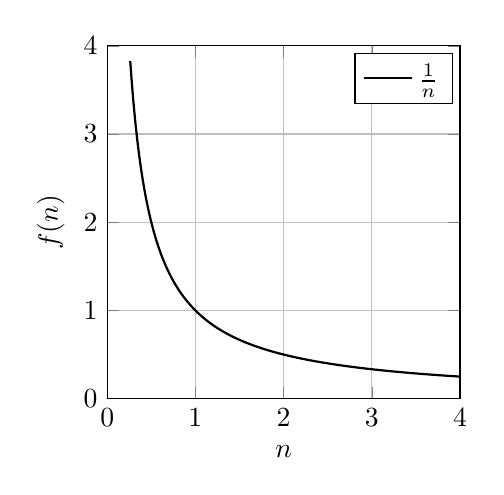
\begin{tikzpicture}
			\begin{axis}[
			xmin=0, xmax=4,
			ymin=0,ymax=4,
			restrict y to domain = 0:4, domain=0:4, width=0.5\textwidth, height=0.5\textwidth, grid=major, samples=200,  ylabel=$f(n)$, xlabel=$n$, legend entries={$\frac{1}{n}$}]
			\addplot[black, thick] {1/x};
			\end{axis}
		\end{tikzpicture}
	\end{center}	
	\item Sulla retta dei numeri reali:
	\begin{tikzpicture}
		\begin{axis}[
		axis y line = none,
		xmin=0, xmax=1,
		ymin=0,ymax=0,
		domain=0:1, width=0.5\textwidth, height=0.1\textwidth]
		\coordinate (zero) at (1,0){};
		\coordinate (uno) at (1/2,0){};
		\coordinate (due) at (1/3,0){};
		\coordinate (tre) at (1/4,0){};
		\coordinate (quattro) at (1/5,0){};
		\end{axis}
		\node [fill = black, circle, inner sep = 1pt, label = north: $1$] at (zero){};
		\node [fill = black, circle, inner sep = 1pt, label = north: $\frac{1}{2}$] at (uno){};
		\node [fill = black, circle, inner sep = 1pt, label = north: $\frac{1}{3}$] at (due){};
		\node [fill = black, circle, inner sep = 1pt, label = north: $\frac{1}{4}$] at (tre){};
		\node [fill = black, circle, inner sep = 1pt, label = north: $\frac{1}{5}$] at (quattro){};
	\end{tikzpicture}
	\item Rapppresentazione dinamica: i mmagino di accendere una lampadina ogni tot secondi e in corrispondenza dell'accensione segno il valore della funzione
\end{itemize}

\subsection{Limite di una successione}
\label{sub:tipilimiti}
Una successione ha 4 possibilità:
\begin{itemize}
	\item $\lim_{n \to \infty} a_n = l \in  \R$ ossia $a_n \to l$
	\begin{itemize}
		\item $\lim_{n \to \infty} a_n = l^{+}$ ossia ha $a_n \ge l$ \underline{definitivamente} 
		\item $\lim_{n \to \infty} a_n = l^{-}$ ossia $a_n \le l$ \underline{definitivamente}
		\item $\lim_{n \to \infty} a_n = l$ oscillando intorno al valore
	\end{itemize}
	\item $\lim_{n \to \infty} a_n = + \infty$ ossia $a_n \to \infty$ 
	\item $\lim_{n \to \infty} a_n = - \infty$ ossia $a_n \to -\infty$
	\item $\lim_{n \to \infty} a_n \quad \text{ NON esiste }$ ossia $a_n$ non ha limite
\end{itemize}
Definizione formale di limite
\definizione{Limite infinito}{Si diche che $a_n \to + \infty$ se \[
\forall M \in  \R \exists a_m \text{ t.c. } a_m\ge M
\] 
ossia $a_m \ge M$ \underline{definitivamente}
\vskip3mm
Si dice che $a_n \to -\infty$ se \[
\forall M \in  \R \exists a_m \le M 
\] 
ossia $a_m \ge M $}

\definizione{Limite se tenda a numero finito}{Si dice che $a_n \to l \in  \R$ \[
 \forall \epsilon \ge 0 \quad l- \epsilon \le a_n \le l+ \epsilon
\] 
ossia 
\[
\left|a_n-l\right| \le \epsilon \quad \text{ \underline{definitivamente} }
\] }

\subsubsection{Errori comuni}
\begin{itemize}
	\item Se $a_n \to \infty$ allora è definitivamente crescente. NO: potrei avere una successione che somma 2 e scende di 1 all'infinito
	\item Se $a_n \to 0$ allora tende o a $0^{+}$ o a $0^{-}$. NO: vedi $\frac{\left( -1 \right) ^{n}}{n}$
	\item Se $a_n$ non è limitata superiormente allora $a_n \to \infty$. NO: vedi $ \left( -2 \right) ^{n}$
\end{itemize}
\subsection{Esempi}
\underline{Esempio 1}
\[
a_n = n^2
\] 
Dimostriamo che $a_n \to \infty$
2 casi:
\begin{itemize}
	\item Se $M \le 0 $ \rarr $ n^2 \ge M$ sempre
	\item Se $M \ge 0 $ \rarr $n^2 \ge M \Leftrightarrow n \ge \sqrt{M} $
\end{itemize}
\underline{Esempio 2}
\[
a_n = \sqrt{n} 
\] 
Dimostriamo che $a_n \to \infty$ 2 casi:
\begin{itemize}
	\item Se $M \le 0 $ \rarr $\sqrt{n} \ge M$ sempre
	\item Se $M \ge 0$ \rarr $\sqrt{n} \ge M \Leftrightarrow n \ge M^2$
\end{itemize}
\bigbox{
\[
\lim_{n \to \infty} n ^{a} = \infty \quad \forall a\ge 0 
\]
}
\underline{Esemipio 3}
\[
\lim_{n \to \infty} \frac{1}{n} = o^{+} 
\] 
Devo verificare che \[
\forall \epsilon > 0 \quad 0 < \frac{1}{n} \ge \epsilon
\] 
\begin{itemize}
	\item $a < \frac{1}{n}$ definitivamente in quanto $n$ è naturale
	\item $\frac{1}{n} \le \epsilon \Leftrightarrow \frac{1}{\epsilon} \le n$
\end{itemize}
\bigbox{
\[
\lim_{n \to \infty}  n ^{\alpha} =0 \quad \forall \alpha \le 0
\] 
}

\teorema{Permanenza del segno}{Se $a_n \to l > 0$ allora $a_n > 0 $ definitivamente\\
Se $a_n \to l<0$ allora $a_n < 0 $ definitivamente}
\underline{Dimostrazione}

\subsection{Unicità del limite}
Una successione ha sempre \underline{solo uno } dei comportamenti descritti in subsec \ref{sub:tipilimiti}
\underline{Dimostrazione}

\begin{itemize}
	\item Supponiamo che uno stesso limite tenda a due cose diverse $a_n \to l_1$ e $a_n \to l_2$ con $l_1 \neq l_2$
	\item Per la definizione di limite il valore del limite deve ricadere in un intorno di $l_1$ e $ l_2$. Se questi due intervalli sono sufficientemente piccoli e dunque non hanno punti in comune dovrei \underline{avere un punto che sta in due parti contemporaneamente}. Ne concludiamo che l'ipotesi sia falsa
\end{itemize}
\subsection{Teoremi sui limiti}
\label{sub:teoremilimiti}
\teorema{Teorema del confronto a 2}{Siano $a_n $ e $b_n$ succesioni. Supponiamo che $a_n \ge b_n$ almeno definitivamente
\begin{itemize}
	\item Se $b_n \to \infty$ allora $a_ n \to \infty$
	\item Se $a_n \to -\infty$ allora $b_n  \to -\infty$
\end{itemize}}
\label{teoconfrontoadue}
\teorema{Teorema del confronto a 3 (dei due carabinieri)}{Siano $a_n, b_n, c_n$ successioni tali che $a_n \le b_n \le c_n$ almeno definitivamente. Supponiamo che $a_n \to l \in  \R$ e $c_n \to l \in  \R$ allora $ b_n \to l \in  \R$}
\label{teoconfrontoatre}
\subsection{Errori comuni}
\begin{itemize}
	\item Supponiamo che a $a_n > b_n$ e $a_n \to l_1, b_n \to l_2$. Allora \[
	l_1 > l_2
	\] 
	\item \underline{Falso} in quanto al limite non si conserva l'uguale. Vedi ad esempio:
	\[
	a_n = \frac{2}{n} \quad b_n = \frac{1}{n}
	\] 
	nonostante i termini di $a_n$ siano sempre il doppio di quelli di $ b_n$ il loro limite è lo stesso e vale 0. Posso in caso affermare che se $a_n > b_n$ allora $l_1 \ge l_2$
\end{itemize}

\subsection{Retta reale estesa}
\label{sub:rettarealeestesa}
\[
\overline{\R} = \R \cup \left\{ +\infty \right\} \cup \left\{ - \infty \right\} 
\] 
\teorema{Somma, prodotto e divisione limiti}{Siano $a_n$ e $b_n$ successioni reali. \[
a_n \to l_1 \in  \R \text{ e } b_n \to l_2 \in  \R
\] 
allora 
\begin{align*}
a_n + b_n &\to l_1 + l_2 & a_n - b_n &\to l_1-l_2\\
a_n b_n & \to l_1l_2 & \frac{a_n}{b_n} &\to \frac{l_1}{l_2}\\
a_n^{b_n} & \to l_1^{ l_2}
\end{align*}

A meno che non si cada in uno di questi 7 casi speciali:
\begin{gather*}
	+\infty - \infty \quad 0 \cdot \left( \pm \infty \right) \frac{0}{0} \quad  \frac{\pm \infty}{\pm \infty}\\
\quad 0^{0} \quad \left( + \infty \right) ^{0} \quad 1^{\pm \infty}\\
\end{gather*}
}
NB: nel caso della successione di tipo $\frac{a_n}{b_n}$ devo stare attento al modo in cui $b_n$ tende a zero: può tendere a $a^{+}, 0 ^{-}$ o a $0$

\subsection{Forma indeterminata}
\textbf{Esempio 1}
\[
a_n = \underbrace{n^3}_{+ \infty} + \underbrace{n^2}_{+\infty} \to + \infty
\] 
\textbf{Esempio 2}
\[
a_n = \underbrace{n^3}_{+ \infty} -  \underbrace{n^2}_{+\infty} = \underbrace{n^2}_{\infty} \underbrace{\left( n-1 \right)}_{+\infty-1}  \to + \infty
\] 
\textbf{Esempio 3}
\[
a_n= \underbrace{\sqrt{n}}_{+\infty} - \underbrace{\frac{1}{n^3}}_{0} \to + \infty
\]
\textbf{Esempio 4}
\[
a_n = 2^{n}
\] 
Dimostro con \underline{disuguaglianza di Bernoulli}(sub \ref{sub:disbernoulli}):
\[
2^{n} \ge n+1
\] 
dunque visto che $ n+1 \to \infty$ allora anche $2^{n} \to \infty$ per \underline{teorema del confronto a 2}(teo \ref{teoconfrontoatre})

\textbf{Esempio 5} 
\[
\lim_{n \to \infty} \frac{\arctan \left( 2^{n} + n! \right) }{n^2 + 3} = 0
\] 
\[
\lim_{n \to \infty} \frac{\sin\left( n \right)}{n}  = 0
\] 
in quanto al numeratore ho valoni finiti e al demonimatore valori infiniti. Posso applicare teorema dei dure carabinieri:
\begin{itemize}
	\item $0 \le \arctan \left( 2^{n} + n! \right) \le \pi$
	\item Diviso per $ n^2 + 3$
	\[
	0 \le \frac{\arctan \left( s^{n} + n! \right) } {\underbrace{n^2 + 3}_{\to 0}} \le \frac{\pi}{\underbrace{n^2 + 3}_{\to 0}}
	\]
	\item Il mio limite deve essere compreso fra $0$ e $0$, quindi è $=0$ per il teorema del confronto a tre (teo \ref{teoconfrontoatre})
\end{itemize}
\textbf{Esempio 6}
\[
\lim_{n \to \infty} \frac{\sqrt{n} - \sqrt[3] {n} }{n + 10^{23}} = \frac{n^{\frac{1}{2}}\left( 1- n^{-6} \right)}{n}  = \frac{1}{\sqrt{n} }\left( 1-n^{-6} \right) \to 0
\] 
\subsection{Implicazione i mportante disuquaglianza di bernoulli}
Dimostro che 
\[
\lim_{n \to \infty} a ^{ n} = + \infty \quad \forall a > 1
\] 
\begin{itemize}
	\item Noto che 
	\[
	a^{n}= \left( 1 + \left(  a-1 \right)  \right) ^{n}
	\] 
	\item questa quantità per il teorema di bernoulli è maggiore di:
	\[
	\left( 1 + \left( a-1 \right)  \right) ^{n} \ge 1 + n\left( a-1 \right) 
	\] 
	\item Se $a > 1$ $\lim_{n \to \infty} n\left( a-1 \right) = + \infty $
\end{itemize}
Se invece ho $a \in  \left( 0,1 \right) $
\[
\lim_{n \to \infty} a^{n} \quad \text{  con  }a \in  \left( 0,1 \right)  
\]
Visto che $a \in  \left( a,1 \right) $ posso supporre che $a=\frac{1}{b}$ con $b > 1$
\[
a^{n} = \left( \frac{1}{b} \right) ^{n} = \frac{1}{b^{n}} \to 0
\] 
\section{Fattoriali e combinatoria}
\definizione{Fattoriale di un numero}{Il fattoriale di un numero è definito nel seguente modo:
\[
0! = 1
\] 
\[
\left( n+1 \right) ! = \left( n+1 \right) \cdot n!
\] 
in numeri $ n!$ rapprentenza il numero di modi in cui posso ordinare $n$ oggetti
}
Per scegliere n persone posso pensare che 
 \begin{itemize}
	\item La prima persona la posso scieglere in $n$ modi
	\item La seconda in $n-1$
	\item La terza in $n-2$
	\item \ldots la k esima in $n-k+1$
\end{itemize}
quindi
\begin{table}[h!]
	\centering
	\begin{tabular}{|c|c|c|c|c|}
	\hline
	n & n-1 & n-2 & \ldots & n-k+1 \\
	\hline
	\end{tabular}
\end{table}

\definizione{Coefficiente binomiale}{
Dati 2 interi $n,k \quad 0 \le k\le n$, ponto \[
\binom{n}{k}= \frac{n!}{k! \left( n-k \right) !}
\]  
}
Immagino di avere un esercito di $n$ soldati e ne devo estrarre k. Non conta l'ordine con cui gli estraggo
\begin{itemize}
	\item Il primo soldato lo posso scegliere in $n$ modi
	\item Il secondo in $n-1$
	\item Il terzo in $n-2$
	\item \ldots il k esimo in $n-k+1$
	\item Devo poi dividere per il le permutazioni possibili visto che \underline{l'ordine non conta}
	\[
	\text{ numero modi di estrarre } = \frac{n\left( n-1 \right) \left( n-2 \right) \ldots \left( n-k+1 \right)}{k!} = \binom{n}{k}
	\] 
	\item Perchè diviso? Pensa al fatto che ogni squadra estratta può essere disposta in $k!$ modi, quindi $k!$ modi vanno considerati come la stessa squadra
\end{itemize}
\subsection{Proprietà dei fattoriali}
\begin{itemize}
	\item Scontate:
	\begin{align*}
	\binom{n}{0} &=  \frac{n!}{0!n!}= 1 &  \binom{n}{n}&=  \frac{n!}{n!0!}= 1 \\
	\binom{n}{1} &=  \frac{n!}{1!\left( n-1 \right) !}=  \frac{n \left( n-1 \right) !}{\left( n-1 \right) }=n &  \binom{n}{n-1} &= \frac{n!}{\left( n-1 \right) 1!}= \frac{n\left( n-1 \right) !}{\left( n-1 \right) !}=n
	\end{align*}
	\item Simmetrica: prendere $k$ persona da squadra di $n$ è la stessa cosa che lasciarne fuori $n-k$ :
\[
\binom{n}{k}= \binom{n}{n-k}
\] 
	\item Generazione ricorsiva binomiale:
	\[
	\binom{n+1}{k+1} = \binom{n}{k} + \binom{n}{k+1}
	\]
	Dimostrazione
		\begin{align*}
		\binom{n}{k} + \binom{n}{k+1} &=  \frac{n!}{k! \left( n-k \right) !} + \frac{n!}{\left( k+1 \right) \left( n-k-1 \right) !}\\
		&= \frac{n!}{k! \underbrace{\left( n-k \right)}_{\left( n-k \right) \left( n-k-1 \right) !} !} + \frac{n!}{\underbrace{\left( k+1 \right)}_{\left( k+1 \right) k!} \left( n-k-1 \right) !} \\
		&= \frac{n!}{k! \left( n-k-1 \right) !} \frac{k+1 +n-k}{\left( n-k \right) \left( k+1 \right) }
		\end{align*}
A livello combinatorio
\begin{itemize}
	\item Prendo un gruppo di $n$ persone e tengo separatamente 1
	\item Per formare un gruppo grande $k+1$ posso:
	\begin{enumerate}
		\item Creare un gruppo grande $n$ e poi aggiungerci il nuovo arrivato
		\item Creare un gruppo grande $n+1$ che non contenga il nuovo arrivato 
	\end{enumerate}
	\item Nel primo caso posso creare $ \binom{n}{k}$ gruppi
	\item nel secondo caso posso create $ \binom{n}{k+1}$ gruppi
\end{itemize}
\end{itemize}
\subsection{Il triangolo di tartaglia}
	\begin{center}
		\includegraphics{Images/Tartaglia.pdf}
	\end{center}
Ogni valore è dato dalla somma dei valori dei termini \underline{sopra} di esso a \underline{sinistra e a destra}
\bigbox{Il coefficiente alla riga n nella posizione k è dato da \[
\binom{n}{k}
\] 
visto che il coefficiente nella posizione $n+1, k+1$ è uguale al coefficiente nella posizione $n, k$ e $n, k+1$ noto che questo triangolo verifica la generazione ricorsiva binomiale:
\[
\binom{n+1}{k+1}= \binom{n}{k} + \binom{n}{k+1}
\]
}
\bigbox{
Nello sviluppo di un binomio del tipo $\left( x+y \right) ^{n}$ il monomio $x^{k}y^{n-k}$ ha coefficiente $ \binom{n}{k}$ ossia:
\[
\left( x+y \right) ^{n} = \sum_{k=0}^{n} \binom{n}{k}x^{k}y^{n-k}
\] 
}
\bigbox{
La somma dei coefficienti alla riga $n$ è uguale a \[
2^{n}
\] 
}

Dimostrazione:
\begin{itemize}
	\item Applico sviluppo del binomio $\left( x+y \right) ^{n}$ con $x=y=1$
	\item In questo caso so che \[
	\left( 1+1 \right) ^{n} = 2^{n}= \sum_{k=0}^{n} \binom{n}{k}1^{k}1^{n-k}= \sum_{k=0}^{n} \binom{n}{k}
	\] 
\end{itemize}
\section{3 criteri: rapporto, radice, rapporto-radice}
\subsection{Criterio della radice}
\begin{itemize}
	\item Sia $a_n$ una successione tale che $a_n \ge 0 $ definitavente
	\item Supponiamo che se $\sqrt[n]{a_n} \to l \in  \R \cup \left\{ +\infty \right\} $ allora ho 3 possibilità:
	\begin{itemize}
		\item se $l > 1$, allora $ a_n \to +\infty$
		\item se $l < 1$, allora $a_n \to 0$
		\item se  $l=1$ il criterio non fornisce informazioni 
	\end{itemize}
\end{itemize}
\subsection{Criterio del rapporto}
\begin{itemize}
	\item Sia $a_n$ una successione tale che $a_n > 0$ definitivamente
	\item Supponiamo che $\lim_{n \to \infty} \frac{a_n+1}{a_n}=l \in  \R \cup    \left\{ +\infty \right\} $
	allora ho 3 possibilità
	\begin{itemize}
		\item se $l > 1$, allora $ a_n \to +\infty$
		\item se $l < 1$, allora $a_n \to 0$
		\item se  $l=1$ il criterio non fornisce informazioni 
	\end{itemize}
\end{itemize}
\subsection{Criterio rapporto $ \rightarrow $ radice}
\begin{itemize}
	\item Sia $a_n$ una successione tale che $a_n > 0 $ definitivamente
	\item Supponiamo che $\frac{a_{n + 1}}{a_n} \to l \in  \R \cup \left\{ +\infty \right\} $
allora
\[
\sqrt[n]{a_n} \to l
\] 
ossia $\frac{a_{n +1}}{a_n}$ e $\sqrt[n]{a_n} \to l$ tendono allo stesso $l \in \R \cup \left\{ +\infty \right\} $
\end{itemize}
\subsection{Dimostrazioni}
\subsubsection{Dimostrazione criterio radice}
\begin{itemize}
	\item Prendo punto a metà fra 1 e $l$
	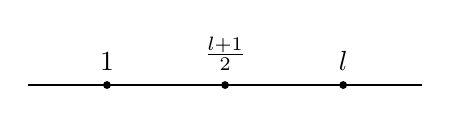
\begin{tikzpicture}
			\node [label=north: 1 , fill=black, circle, inner sep = 1pt] at (0,0) {};
			\node [label=north: $l$ , fill=black, circle, inner sep = 1pt] at (3,0) {};
			\node [label=north: $\frac{l+1}{2}$ , fill=black, circle, inner sep = 1pt] at (1.5,0) {};
			\draw (-1,0) to (4,0);
	\end{tikzpicture}
	\item Visto che $\sqrt[n]{a_n} \to l$ necessariamente 
	\[
	\sqrt[n]{a_n} \ge \frac{l+1}{2}
	\] 
	\item Ho quantità positive sia a sinistra che a destra, posso elevare alla $n$ da entrambe le parti, ottenendo:
\[
a_n \ge \left( \frac{l+1}{2} \right) ^{n}
\] 
	\item Se $l > 1$ $\left( \frac{l+1}{2} \right)^{n}  \to \infty$
\end{itemize}
\hr
se invece $l<1$ agisco nello stesso modo:
\begin{itemize}
	\item Prendo punto a metà fra $l$ e 1
	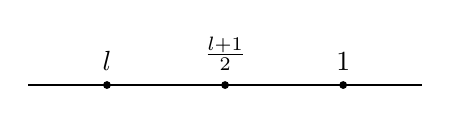
\begin{tikzpicture}
			\node [label=north: 1 , fill=black, circle, inner sep = 1pt] at (3,0) {};
			\node [label=north: $l$ , fill=black, circle, inner sep = 1pt] at (0,0) {};
			\node [label=north: $\frac{l+1}{2}$ , fill=black, circle, inner sep = 1pt] at (1.5,0) {};
			\draw (-1,0) to (4,0);
	\end{tikzpicture}
	\item Visto che $\sqrt[n]{a_n} \to l$ necessariamente 
	\[
	\sqrt[n]{a_n} \le \frac{l+1}{2}
	\] 
	\item Ho quantità positive sia a sinistra che a destra, posso elevare alla $n$ da entrambe le parti, ottenendo:
\[
a_n \le \left( \frac{l+1}{2} \right) ^{n}
\] 
	\item Se $l < 1$ $\left( \frac{l+1}{2} \right)^{n}  \to 0$
	\item Siccome $a_n \ge 0$ per ipotesi allora 
	\[
	0 \le a_n \le \left( \frac{l+1}{2} \right) ^{n}
	\] 
	ossia $a_n \to 0$ per teorema del confronto a tre
\end{itemize}
\subsection{Numero di nepero}
\bigbox{
Il numero di nepero è definito dal seguente limite
\[
\lim_{n \to \infty} \left( 1+\frac{1}{n} \right) ^{n} 
\] 
}
\subsection{Esempio forme indeterminate}
\textbf{Esempio 1}
\[
\lim_{n \to \infty} \frac{n^{n}}{n!} = + \infty
\]
Criterio del rapporto:
\[
\frac{a_{n+1}}{a_n} = \frac{\left( n+1 \right) ^{n+1}}{\left( n+1 \right) !} \cdot\frac{n!}{n^{n}}
\] 
\textbf{Esempio 2}
\[
\lim_{n \to \infty} \frac{3^{n^{2}}}{n!} = +\infty
\]
Criterio del rapporto:
\[
\frac{a_{n+1}}{a_n} = \frac{3^{\left( n+1 \right) ^{2}}}{\left( n+1 \right) !}
\] 
\textbf{Esempio 3}
\[
\lim_{n \to \infty} \frac{\sqrt[n]{n!} }{n} = 
\] 
Criterio rapporto radice
\[
\frac{\sqrt[n]{n!} }{n} = \sqrt[n]{\frac{n!}{n^{n}}} 
\]
\section{Limiti di funzioni}
\definizione{Limite di funzione}{
Data una funzione $f : A \rightarrow \R \quad  A \subseteq \R$ abbiamo tre tipologie di limite:
\[
\lim_{x \to \infty} f(x) \quad \lim_{x \to -\infty} f(x) \quad \lim_{x \to x_0} f(x)  
\] 
\textbf{Primo tipo:}
\[
\lim_{x \to \infty} f(x) = \begin{cases}
	l \in \R\\
	+ \infty \\
	- \infty \\
	\text{ non esiste }
\end{cases}
\] 
se $ \lim_{x \to \infty} f(x) = + \infty$: 
\[
\forall M \in  \R \quad \exists k \in  \R \text{ t.c. } f\left( x \right) \ge M \forall x \ge k
\] 
se $ \lim_{x \to \infty} f(x) = + -\infty$: 
\[
\forall M \in  \R \quad \exists k \in  \R \text{ t.c. } f\left( x \right) \le M \forall x \ge k
\] 
se $ \lim_{x \to \infty} f(x) = l$: 
\[
\forall \epsilon > 0 \quad \exists k \in  \R \text{ t.c. } l- \epsilon \le f\left( x \right) \le l+ \epsilon \quad \forall x \ge k
\] 
ossia 
\[
\left|f\left( x \right) -l\right| \le \epsilon
\] 
se $ \lim_{x \to \infty} f(x) = l^{+}$: 
\[
\forall \epsilon > 0 \quad \exists k \in  \R \text{ t.c. }  l <  f\left( x \right) \le l+ \epsilon \quad \forall x \ge k
\] 
se $ \lim_{x \to \infty} f(x) = l^{-}$: 
\[
\forall \epsilon > 0 \quad \exists k \in  \R \text{ t.c. }  l-\epsilon \le f\left( x \right) \le l \quad \forall x \ge k
\] 
\textbf{Secondo tipo}: molto simile a primo, semplicemnte speculare
\vskip3mm
\textbf{Terzo tipo:}
\[
\lim_{x \to x_0} f(x) =
\begin{cases}
	l \in  \R \\
	+ \infty\\
	-\infty
	\text{ non esiste }
\end{cases}
\]
se $\lim_{x \to x_0} f(x) = + \infty$:
\[
\forall M \in  \R \quad \exists \delta > 0 \text{ t.c. } f\left( x \right)  \ge M \quad \forall x \in \left[ x_0-\delta, x_0+\delta \right] \setminus \left\{ x_0 \right\}  
\] 
se $\lim_{x \to x_0} f(x) = l \in  \R$:
\[
\forall \epsilon >0 \quad \exists \delta > 0 \text{ t.c. } \left|f\left( x \right) -l \right|\le \epsilon \text{ se } x \in \left[ x_0- \delta, x_0+ \delta \right] \setminus \left\{ x_0 \right\} 
\] 
}
\subsection{Continuità}
\definizione{Continuità}{
Una funzione $ f: A \rightarrow \R \text{ con } A \subseteq \R$ si dice continua in un punto $x_0 \in  A$ se:
\[
\lim_{x \to x_0} f(x) = f\left( x_0 \right) 
\] 
}
OSS:
\begin{itemize}
	\item Si dice che $f$ è continua in $A$ se essa è continua in ogni punto di $A$
	\item Le funzioni elementari sono sempre comtinue sul loro dominio
	\item Se faccio operazioni algebriche su funzioni continue ottengo funzioni continue
	\item La composizione di funzioni continue è continua
\end{itemize}
\subsection{Limiti notevoli}
Limiti "nonni"
\begin{gather}
	\lim_{x \to 0} \frac{\sin\left( x \right) }{x} = 1 \\
	\lim_{x \to + \infty} \left( 1+\frac{1}{x} \right) ^{x} = e
\end{gather}
Limiti "di seconda generazione"
\begin{align*}
	& \lim_{x \to 0} \frac{1-\cos\left( x \right) }{x^2} = \frac{1}{2} &\lim_{x \to 0} \frac{e^{x}-1}{x}=1 \\
	& \lim_{x \to 0} \frac{\log\left( 1+x \right) }{x}=1 &\lim_{x \to -\infty} \left( 1+\frac{1}{x} \right) ^{x} = e\\
	& \lim_{x \to 0} \frac{ \tan \left( x \right) }{x}=1  & \lim_{x \to 0} \frac{\arctan \left( x \right) }{x} = 1  \\
	& \lim_{x \to 0} \frac{\arcsin \left( x \right) }{x} = 1 & \lim_{x \to 0} \frac{a^{x}-1}{x}= \log \left( a \right) \\
	& \lim_{x \to 0^{+}} x \log \left( x \right) =0
\end{align*}
\subsection{Cambio di variabile}
\textbf{Esempio 1} 
\[
\lim_{x \to 0} \frac{\sin\left( x^2 \right) }{x^2} 
\] 
pongo $y=x^2$ 
\[
\lim_{x \to 0} \frac{\sin\left( x^2 \right) }{x^2}= \lim_{y \to 0} \frac{\sin\left( y \right) }{y}= 1 
\] 
\textbf{Esempio 2}
\[
\lim_{x \to  0} \frac{e^{\sin\left( x \right) }-1}{\sin\left( x \right) } 
\] 
pongo $y=\sin\left( x \right) $ ; se $x \to 0 \Rightarrow \sin\left( x \right) \to 0 \Rightarrow y \to 0$ 
\[
\lim_{x \to 0} \frac{e^{\sin\left(  \right) -1}}{\sin\left( x \right) }= \lim_{y \to 0} \frac{e^{y}-1}{y}  
\] 
\textbf{Esempio 3}
\[
\lim_{x \to \pi } \frac{\log\left( 1+\sin\left( x \right)  \right) }{\sin\left( x \right) } 
\] 
pongo $y=\sin\left( x \right) $ ; se $x \to \pi \Rightarrow \sin\left( x \right) \to 0 \Rightarrow y \to 0$
\[
\lim_{x \to \pi } \frac{\log\left( 1+\sin\left( x \right)  \right) }{\sin\left( x \right) } = \lim_{y \to 0} \frac{\log \left( 1+y \right) }{y} 
\] 
\textbf{Esempio 4}
\[
\lim_{x \to 0} \frac{1-\cos\left( x \right) }{x^2} 
\]
moltiplico e divido per $1+\cos\left( x \right) $ 
\[
\lim_{x \to 0} \frac{1-\cos\left( x \right) }{x^2} = \lim_{x \to 0} \left(\frac{1-\cos\left( x \right) }{c^2} \cdot \frac{1+ \cos \left( x \right) }{1 + \cos \left( x \right) } \right) = \lim_{x \to 0} \frac{1-\cos ^2 \left( x \right) }{x^2} \cdot \frac{1}{1+\cos\left( x \right) }  = 
\]
\[
=\lim_{x \to 0} \left( \frac{\sin \left( x \right) }{x} \right) ^2 \cdot \frac{1}{1+\cos\left( x \right) } = 1 \cdot \frac{1}{2}
\]
\textbf{Limite}
\[
\lim_{x \to 0} \frac{e^{x} -1}{x}
\] 
pongo $ x = \log \left( y+1 \right) $ 
\[
 \lim_{y \to 0} \frac{y}{\log \left( 1+y \right) }  = \lim_{x \to 0} \frac{1}{\underbrace{\frac{\log\left( 1+ y\right) }{y}}_{\text{limite notevole}}} 
\] 
\textbf{Limite}
\[
\lim_{x \to 0} \frac{e^{x}-1}{x} 
\] 
pongo $a^{x}=x \log \left( a \right) $
\[
\frac{e^{x \log \left( a \right)  }}{x} \cdot  
\] 
\subsection{Ordini di infiniti}
\bigbox{
\[
\lim_{x \to \infty} \frac{\left( \log \left( x \right)  \right) ^{a}}{x^{b}}=0 \quad \forall e>0, b>0
\] 
}
dimostro facendo cambiodi variabile (im pongo $y= \log \left( x \right) $)
\bigbox{
\[
\lim_{x \to 0^{+}} x \log \left( x \right) = 0
\] 
}
pongo $y=\frac{1}{y}$

\subsection{Dimostrazioe $\lim_{x \to 0} \frac{\sin\left( x \right) }{x} $}
\begin{itemize}
	\item Sappaimo che vale la seguente disuguaglianza:
	\[
	\sin \left( x \right) \le x \le \tan \left( x \right) 
	\] 
	\item Divido per $\sin\left( x \right) $
	 \[
	 1 \le \frac{x}{\sin\left( x \right) }\le \frac{1}{\cos\left( x \right) }
	 \] 
\end{itemize}
\subsection{Altri esempi}
\textbf{Esempio 1}
\[
\lim_{x \to  0} \frac{\log \left( \cos \left( x \right)  \right) }{x^2}  
\]
\begin{itemize}
	\item
	\[
\lim_{x \to  0} \frac{\log \left( \cos \left( x \right)  \right) }{x^2}  = \lim_{x \to 0} \frac{\log\left( \cos \left( x \right) +1 -1 \right) }{x^2} 
	\] 
	\item Moltiplico e divito per $\cos\left( x \right) -1$
	\[
	\lim_{x \to 0} \frac{\log \left( 1+ \left( \cos \left( x \right) -1 \right)  \right) }{\cos \left( x \right) -1} \cdot \frac{\cos \left( x \right) -1}{x^2} 
	\] 
	\item Ottengo due limiti notevoli
\end{itemize}
\textbf{Esempio 2}
\[
\lim_{x \to 0} \left( \cos\left( x \right) \right) ^{\frac{1}{x^2}}  
\] 
\begin{itemize}
	\item Ricordo che $A^{B}=e^{B\log A}$
	\item 
	\[
\lim_{x \to 0} \left( \cos\left( x \right) \right) ^{\frac{1}{x^2}}  = \lim_{x \to 0} e^{\frac{1}{x^2}\log\left( \cos\left( x \right)  \right) } 
	\] 
\end{itemize}
\textbf{Esempio 3}
\[
\lim_{x \to 0} \frac{e^{\tan \left( x \right) }- \cos\left( x \right) + \arctan \left( 2x \right) }{x} 
\]
\begin{itemize}
	\item Sommo e sottraggo 1
\[
\lim_{x \to 0} \frac{e^{\tan \left( x \right) }-1 + 1- \cos\left( x \right) + \arctan \left( 2x \right) }{x} 
\] 
	\item Quindi ottengo limiti notevoli:
	\[
	\lim_{x \to 0} \frac{e^{\tan \left( x \right) }-1}{x}+ \frac{1-\cos\left( x \right) }{x} + \frac{\arctan \left( 2x \right) }{x} 
	\] 
	\item Moltiplico e divido numeratori e demonimatori per ottenere limiti notevoli
\end{itemize}
\textbf{Esempio 4}
\[
\lim_{x \to +\infty} \frac{\log\left( 1+2^{x} \right) }{x} 
\]
\begin{itemize}
	\item Se $x \to + \infty$ l'uno diventa insignificante. Quindi:
	\[
	\lim_{x \to +\infty} \frac{\log\left( 1+2^{x} \right) }{x}= \frac{\log\left( 2^{x} \right) }{x} = \frac{x \log\left( x \right) }{x}  = \log\left( 2 \right) 
	\] 
	\item Rigorosamente potrei raccogliere a fattor comune il $2^{x}$
\end{itemize}
\subsection{Dimostrare non esistenza di un limite}
\definizione{Sottosuccessione}{
Data una successione $a_n$ una sottosuccessione è composta da tuttti i termini \underline{con indice crescente} selezionati secondo una data regola
}
\teorema{Essitenza di un limite di una successione}{
Sia $a_n$ una successione di numeri reali e sia $a_{kn}$ la regola che descrive come scelgo la sottosuccessione. Supponiamo che $a_n \to l \in  \R$ allora 
\[
a_{kn} \to l
\] 
se $a_n$ non ha limite non posso dire nulla riguardo a $a_{nk}$
}
Esempio:
se voglio dimostrare che una successione non ha limite posso cercare due sottosuccessioni che non convergano verso lo stesso limite
\[
e_n = \left( - \right) ^{n} \rightarrow \text{ non ha limite }
\] 
\[
a_{2n}=\left( -1 \right) ^{2n} \rightarrow_1,1,1,1,1 \rightarrow 1
\]
\[
a_{2n+1}= \left( 1 \right) ^{2n+1} = -1,-1,-1,-1,-1, \rightarrow -1
\] 
per questo motivo visto che $l_1 \neq l_2$, $a_n$ non ha limite
\[
a_n=\sin\left( \frac{\pi}{2}n \right) 
\] 
\[
a_{2n}= \sin\left( n \pi  \right) = 0,0,0,0,0 \rightarrow 
\]

\section{Numero di nepero}
Per dimostrare che la successione $a_n = \left( 1+ \frac{1}{n} \right) ^{n}$ converge al numero di nepero servono dei prerequisiti e dei teoremi

\definizione{Crescenza/decrescenza di una successione}{
Una successione $a_n$ si dice:
\begin{itemize}
	\item Debolmente crescente se \quad $a_{n+1} \ge a_n \quad \forall n \in  \N$
	\item Strettamente crescente se \quad $a_{n+1} > a_n \quad \forall n \in  \N$
\end{itemize}
La stessa cosa vale per la decrescenza
}
OSS: una funzione è debolmente crescente se e solo se per ogni $m >n$ anche $a_m \ge a_n$
Consideriamo la successione $e_n = \left( 1+ \frac{1}{n} \right) ^{n}$ 

\teorema{Limiti succesioni crescenti}{
Sia $a_n$ una successione debolmente crescente. Allora abbiamo 2 possibili limiti:
\begin{itemize}
	\item $a_n \to l \in  \R$
	\item $ a_n \to + \infty$
\end{itemize}
In ogni caso il limite della successione è il $sup\left( a_n \right) $
}

\teorema{Corollario al teorema precedente}{
Sia $a_n$ una successione 
\begin{itemize}
	\item Debolemnte crescente 
	\item Limitata superiormente
\end{itemize}
Allora \[
a_n \to l \in  \R
\] 
NB: non necessariamente $l = k$
}
\subsection{Dimostrazione definizione numero di nepero}
La dimostrazione si basa su 3 proprietà della succession $ e_n$
\begin{itemize}
	\item E' sempre $\ge 2 \forall n$
	\item E' debolmente crescente
	\item E' $\le 3 \forall n$
\end{itemize}
se so che $e_n$ è limitata e crescente allora posso affermare che 
\[
e_n \to l \in \left[ 2,3 \right] 
\] 
\textbox{Dimostro un passo alla volta}

 E' sempre $\ge 2 \forall n$
\begin{itemize}
	\item Uso disuguaglianza di Bernoulli ossia 
	\[
	\left( 1+x \right) ^{n} \ge 1+ nx
	\] 
	\item Pongo $x=\frac{1}{n}$ ossia 
	\[
	e_n = \left( 1+\frac{1}{n} \right) ^{n} \ge 1 + n \frac{1}{n} \ge 2
	\] 
\end{itemize}
E' debolmente crescente
\begin{itemize}
	\item \[
	\left( 1+\frac{1}{n} \right)^{n} \ge \left( 1 + \frac{1}{n-1} \right) ^{n-1}
	\] 
	\item \[
	\left( \frac{n+1}{n} \right) ^{n} \ge \left( \frac{n}{n-1} \right) ^{n-1}
	\] 
	\[
	\frac{\left( n+1 \right) ^{n}}{n^{n}} \ge \frac{n^{n-1}}{\left( n-1 \right) ^{n-1}}
	\] 
	\item Moltiplico e divido per $n$ e per $n-1$ il membro di destra
	\[
	\frac{\left( n+1 \right) ^{n}}{n^{n}} \ge \frac{n^{n-1}}{\left( n-1 \right) ^{n-1}} \cdot \frac{n}{n} \cdot \frac{n-1}{n-1}
	\] 
	ottengo quindi
	\[
	\frac{\left( n+1 \right) ^{n}}{n^{n}}\ge \frac{n^{n}}{\left( n-1 \right) ^{n}}\cdot \frac{n-1}{n}
	\] 
	\[
	\frac{\left( n+1 \right) ^{n} \left( n-1 \right) ^{n}}{n^{2n}} \ge \frac{n-1}{n}
	\] 
	\item Noto la somma per differenza al numeratore del primo menmbro
	\[
	\frac{\left( n^2-1 \right) ^{n}}{\left( n^2 \right) ^{n}} = \left( \frac{n^2-1}{n^2} \right) ^{n} = \left( 1 - \frac{1}{n^{2}} \right)^{n}\ge \frac{n-1}{n} = 1 - \frac{1}{n}
	\] 
	\[
	\left( 1 - \frac{1}{n^{2}} \right)^{n} \ge   1 - \frac{1}{n}
	\] 
	\item Pongo x = $-\frac{1}{n^2}$ e moltiplicando e dividendo per $n$ a destra ottengo che

	\[
	\left( 1-\frac{1}{n^2} \right) ^{n} \ge 1- \frac{1}{n} = \left( 1+x \right) ^{n} \ge 1+ nx
	\] 
	\textbox{La crescenza è quindi stata verificata per la disuguaglanza di bernoulli}
\end{itemize}
E' $\le 3 \forall n$
\begin{itemize}
	\item  Utilizzo binomio di Newtoon:
	\[
	\left( x+y \right)^{n} = \sum_{k=1}^{n} \binom{n}{k}x^{k}y^{n-k} = \sum_{k=1}^{n} \binom{n}{k} x^{n-k}y^{k} 
	\] 
	\item Pongo $x=1$ e $y= \frac{1}{n}$ :
	\[
	\left( 1+\frac{1}{n} \right) ^{n}= \sum_{k=1}^{n} \binom{n}{k}1^{n-k}\frac{1}{n^{k}} = \sum_{k=1}^{n} \binom{n}{k} \frac{1}{n^{k}}
\] 
	\item Sviluppando la sommatoria mi accordo di alcune cose:
	\[
	 \binom{n}{0}\frac{1}{n^{0}}  \binom{n}{1} \frac{1}{n} + \binom{n}{2}\frac{1}{n^2}\ldots
	\] 
	\[
	= 1 + 1 + \frac{n \left( n-1 \right) }{2!} \frac{1}{n^2} + \frac{n \left( n-1 \right) \left( n-2 \right) }{3!} \frac{1}{n^3} \ldots
	\] 
	\item Noto che la quantità $ \frac{n\left( n-1 \right) }{n^2}$ è maggiorata da 1. Posso affermare quindi che l'uguaglianza è maggiorata dalla seguente:
	\[
	1+1+\frac{1}{2!}+ \frac{1}{3!}+ \frac{1}{4!}+\ldots+ \frac{1}{n!}
	\] 
	\item Visto che si può dimostrare per induzione che $ n! \ge 2^{n} \forall n \in  \N$ quest'ultima somma sarà a sua volta maggiorata dalla seguente:
	\[
	1+1+\frac{1}{2} + \frac{1}{4} + \frac{1}{8} + \ldots \frac{1}{2^n}
	\] 
	\item Si può dimostrare poi per induzione che $1 + a + a^2 + a^3 + \ldots + a^{n-1} = \frac{1-a^{n}}{1-a}$, quindi nel nostro caso sappiamo che:
	\[
	1+1+\frac{1}{2} + \frac{1}{4} + \frac{1}{8} + \ldots \frac{1}{2^n} = 1+\frac{1-\frac{1}{2^{n}}}{1-\frac{1}{2}} = 3
	\] 
	\item Quindi $a_n \le 3$
\end{itemize}
\bigbox{
Ho dimostrato dunque che
\[
\lim_{x \to \infty} \left( 1+\frac{1}{n} \right) ^{n} = l \in \left( 2,3 \right) 
\] 
}

\section{O-piccolo}
\definizione{O-piccolo definizione 1}{
Una funzione $ f: A \rightarrow \R$ è \underline{o-piccolo per $x \to x_0$} se esiste una funzione $\omega : A ro \R$ tale che 
\[
f\left( x \right) =g\left( x \right) \omega \left( x \right) \text{ e } \lim_{x \to x_0} \omega =0 
\] 
Si scrive che $f\left( x \right) = o\left( g\left( x \right)  \right) $
}
\definizione{O-piccolo definizione 2}{
Supponiamo di poter dividere per $g\left( x \right) $. Assumiamo quindi $g\left( x \right) \neq 0$ tranne tuttalpiù in $x_0$ allora $f\left( x \right) = o\left( g\left( x \right)  \right) $ se e solo se:
\[
\lim_{x \to x_0} \frac{f\left( x \right) }{g\left( x \right) } =0
\] 
}
\subsection{Proprietà o-piccolo}
\textbf{Somma e differenza di o piccoli}

\[
o\left( g \right) + o\left( g \right)  = o \left( g \right) \quad x \to x_0
\] 
\[
o\left( g \right) - o\left( g \right) = o\left( g \right) \quad x \to x_0
\] 

Dimostrazione:
\vskip3mm
Date due funzioni $f_1\left( x \right)  = o\left( g\left( x \right)  \right) \quad x \to x_0$ e $f_2\left( x \right) = o\left( g\left( x \right)  \right) \quad x \to x_0$
\begin{itemize}
	\item $f_2\left( x \right) = g\left( x \right) \omega_2 \left( x \right) $
	\item $f_1\left( x \right) + f_2\left( x \right) = g\left( x \right) \left( \underbrace{\omega_1\left( x \right) + \omega_2\left( x \right) }_{\omega_3 \to 0} \right) $
\end{itemize}

\textbf{Moltiplicazione per scalare}
\[
k o\left( g \right) = o\left( g \right)  \quad  x \to x_0
\] 

\begin{itemize}
	\item $f_1\left( x \right) = g\left( x \right) \omega_1 \left( x \right) $
	\item $kf_1\left( x \right) = g\left( x \right)\cdot k\omega \left( x \right) = g\left( x \right) \omega \left( x \right)  $
\end{itemize}
\textbf{Prodotto di o-piccoli}
\[
o\left( g \right) o\left( g \right) = o\left( g^2 \right) \quad x \to x_0
\] 
\begin{itemize}
	\item $o\left( g \right) o\left( g \right) = f\left( x \right) f\left( x \right) \omega \left( x \right) \omega \left( x \right)= \left( f\left( x \right) \right) ^2 \omega \left( x \right) ^2 $
	\item $= g^2 \omega \left( x \right) = o\left( g^2 \right)  $
\end{itemize}
\textbf{Transitività o-piccolo}
\begin{gather*}
	f\left( x \right) = o\left( g\left( x \right)  \right) \quad x \to x_0 \\
	g\left( x \right) = o\left( h\left( x \right)  \right) \quad x \to x_0	\\
	\text{ allora }\\
	f\left( x \right) = o\left( h\left( x \right)  \right) \quad x \to x_0
\end{gather*}
\textbf{Prodotto per scalare dell'argomento}
\begin{gather*}
	\text{ se }f\left( x \right) = o\left( g\left( x \right)  \right) \quad x \to 0\\
	\text{ allora }\\
	f\left( kx \right) = o\left( g\left( kx \right)  \right) 
\end{gather*}
\subsection{Sviluppi al primo ordine}
Mentre faccio un limite \underline{per $x \to 0$} posso usare gli sviluppi al primo ordine per rendre tutto molto più semblice:
\begin{align*}
	\sin\left( x \right) &= x + o\left( x \right) & e^{x}&= 1 + x + o\left( x \right) \\
	\cos\left( x \right)&=  1 + o\left( x \right) & \log\left( 1 + x \right) &= x + o\left( x \right) \\
	\cos\left( x \right)  &=  1 + \frac{x^2}{2} + o\left( x^2 \right) & \arctan\left( x \right) &= x + o\left( x \right) \\
	\tan\left( x \right) &=  x + o\left( x \right) & \arcsin \left( x \right) &=  x + o\left( x \right) 
\end{align*}
Posso dimostrarli tutti isolando il $o\left( x \right) $ e facendo il limite per $x \to 0$ di $\frac{f\left( x \right) }{f\left( x \right) }$
\section{Derivate}
\definizione{Derivata con rapporto incrementale}{
In un punto $x_0$ di una funzione la derivata è definita tramite il rapporto incrementale:
\[
	f' \left( x_0 \right) = \lim_{h \to 0} \frac{f\left( x_0 + h \right) - f\left( x_0 \right) }{h} = \lim_{x \to x_0} \frac{f\left( x \right) - f\left( x_0 \right)}{x-x_0}   
\] 
$f\left( x \right) $ è derivabile in $x_0$ se il limite \underline{esiste} ed è \underline{finito}
}
\definizione{Derivata con o piccolo}{
	Dire che esiste la derivata $f' \left( x_0 \right) $ è equivalente a dire che è siddisfatta la seguente relazione:
	\[
		f\left( x_0 + g \right) = f\left( x_0 \right) + f'\left( x_0 \right) h + o\left( h \right) \quad \text{ con } h \to 0	
	\] 
}
Dimostrazione fra le due definzioni:
\begin{itemize}
	\item Supponiamo vera la relazione con l'o piccolo e inseriamola all'interno del rapporto incrementale:
		\[
			f'\left( x_0 \right)  = \frac{f'\left( x_0 +h\right) - f\left( x_0 \right) }{h} = \frac{f'\left( x_0 \right) h + o\left( h \right) }{h} = f'\left( x_0 \right) + \underbrace{\frac{o\left( h \right) }{h}}_{ \to 0 } = f'\left( x_0 \right) 
		\]  
	\item Viceversa: supponiamo vero il limite del rapporto incrementale. Dimostro che 
		\[
			o\left( h \right)  = f\left( x_0 + h \right) - f\left( x_0 \right) - f'\left( x_0 \right) h
		\] 
	\item Calcolo $\lim_{h \to 0} \frac{f\left( h \right) }{g\left( h \right) }$
		\[
			\frac{f\left( x_0+h \right) - f\left( x_0 \right) - f'\left( x_0 \right) h}{h} = \frac{f\left( x_0 +h \right) - f\left( x_0 \right)}{h} - f'\left( x_0 \right) = f'\left( x_0 \right) - f' \left( x_0 \right) =0  
		\] 
\end{itemize}
Quindi le due relazioni sono \underline{reciprocamente implicate}
\subsection{Regole derivazione}
\begin{align*}
	\left( f \pm g \right) ' &= f' \pm g' & \left( \lambda f \right) ' &=  \lambda f'\\
	\left( fg \right) '	&=  f'g + fg' & \left( \frac{f}{g} \right) ' &=  \frac{f'g- g'f}{g^2}\\
	\left( f\left( g\left( x \right)   \right)  \right) '  &=  f'\left( g \right) g'
\end{align*}
\subsubsection{Dimostrazione regole di derivazione}
\[
	\boxed{	\left( fg \right) ' =  f'g + fg'}
\]
\begin{itemize}
	\item Per definizione la derivata è il limite del rapporto incrementale:
		\[
			f'\left( f\left( x \right) g\left( x \right)  \right) = \lim_{h \to 0} \frac{f\left( x_0 +h \right) g\left( x_0+h \right) - f\left( x_0 \right) g\left( x_0 \right) }{h} 
		\] 
	\item Aggiungo e sottraggo $f\left( x_0 +g \right) g\left( o \right) $ 
		\[
			\frac{f\left( x_0+h \right) \underbrace{- f\left( x_0 + h \right) g\left( x_0 \right) + g\left( x_0 + h \right) g\left( x_0 \right)} - f\left( x_0 \right) }{h}
		\] 
	\item Raccolgo primo con secondo e terzo con quarto:
		\[
			f\left( x_0 + h \right) \frac{g\left( x_0 +h \right) - g\left( x_0 \right) }{h} + g\left( x_0 \right) \frac{f\left( x_0 + h \right) - f\left( x_0 \right) }{h}
		\] 
	\item tutto questo è uguale a: 
		\[
			f\left( x_0 \right) g' \left( x_0 \right) + g\left( x_0 \right) f'\left( x_0 \right) 
		\] 
		Questo in quanto $f$ è continua
\end{itemize}
\[
	\boxed{	\left( f\left( g\left( x \right)   \right)  \right) '  =  f'\left( g \right) g'}
\]
\begin{itemize}
	\item 
	i
\end{itemize}
\subsection{Derivate elementari}
\begin{align*}
	&\left( \tan x \right) ' = \frac{1}{\cos ^2 x}=  1 + \left( \tan x \right) ^2 && \left( \arctan  \right) ' =  \frac{1}{1+x^2}\\
	&\left( \arcsin \right) ' =  \frac{1}{\sqrt{1-x^2} }  &&\left( \arccos \right) ' =  -\frac{1}{\sqrt{1-x^2} }\\
	&\left( a^{x} \right) ' =  a^{x} \cdot \log a  
\end{align*}
\subsubsection{Dimostrazione di derivate elemenrari tramite o-piccolo}
\[
	\boxed{	d\left[ e^{x} \right] = e^{x}}
\]
\begin{itemize}
	\item $f\left( x_0 + h \right) = e^{x_0 + h}= e^{x_0 }e ^{ h}$
	\item Applico sviluppi al primo ordine:
		\[
			e^{x_0 }e ^{ h}= e^{x_0}\left( 1+h+ o\left( h \right)  \right) = e^{x}+ e^{x_0}h + e^{x_0}o\left( h \right) 
		\] 
	\item Noto che
		\[
			\underbrace{e^{x}}_{f\left( x_0 \right) }+ \underbrace{e^{x_0}}_{f'\left( x_0 \right) }h + \underbrace{e^{x_0}o\left( h \right)}_{=o\left( h \right) }
		\] 
\end{itemize}
\[
	\boxed{	d\left[ \sin \left( x \right)  \right] }
\]
\begin{itemize}
	\item $f\left( x_0 + h \right) = \sin \left( x_0 + h \right) $
	\item Applico formula somma di seni:
		\[
			\sin \left( x_0 +h \right) = \sin \left( x_0  \right) \cos \left( h \right) + \cos \left( x_0 \right) \sin \left( h \right) 
		\] 
	\item Applico sviluppo al primo ordine di $\sin \left( h \right)$ e $\cos \left( h \right) $
		\[
			\sin \left( x_0 \right) \left( 1+ o\left( h \right)  \right) + \cos \left( x_0 \right) \left( h + o \left( h \right)  \right) 
		\] 
\end{itemize}
\[
	\boxed{	d\left[ \log \left( x_0+h \right)  \right] 
}
\]
\begin{itemize}
	\item $f\left( x_0 + h \right) = \log \left( x_0 +h \right) $
	\item Raccolgo $x_0$ :
		\[
			\log \left( x_0 \left( 1+ \frac{h}{x_0} \right)  \right) 
		\] 
	\item Proprietà dei logaritmi:
		\[
			\log \left( x_0 \right) + \log \left( 1 + \frac{1}{x_0} \right) 
		\] 
	\item Sviluppo al primo ordine di $\log  \left( 1 + \frac{h}{x_0} \right) $ :
		\[
			\log \left( x_0  \right) + \frac{h}{x_0}+ o\left( \frac{h}{x_0} \right) 
		\] 
	\item Per proprietà degli o piccoli $o\left( \frac{h}{x_0} \right) = o\left( h \right) $
	\[
		\underbrace{\log \left( x_0 \right)}_{f\left( x_0 \right) } + \underbrace{\frac{1}{x_0}h}_{f'\left( x_0 \right) } + o\left( h \right) 
	\] 
\end{itemize}
\section{De l'Hopital e Taylor: pilastri della matematica}
\subsection{De l'hopital}
\subsection{Esempi limiti}

\[
	\frac{x - \sin  \left( x \right)  + x^{5}}{x^{3}}
\] 
	 Applico de l'Hopital derivando 3 volte
	 \begin{align*}
		\frac{x - \sin  \left( x \right)  + x^{5}}{x^{3}} &= \\
		&= \lim_{x \to 0} \frac{x - \sin \left( x \right)  + x^{5}}{x^3}   \\
		&= \lim_{x \to 0} \frac{1 - \cos \left( x \right)  + 5x^{4}}{3 x ^2}\\
		&= \lim_{x \to 0} \frac{\sin \left( x \right)  + 20 x^3}{6x} \\
		&=\lim_{x \to 0} \frac{\cos \left( x + 60x^2 \right) }{6} 
	 \end{align*}

\subsection{Taylor}
\teorema{Formula di taylor}{
	Sia $f $ unf funzione e sia $n \in  \N$. Sotto opportune ipotesi esiste un polinomio di grado $\le n, P_n \left( x \right) $ tale che 
	\[
		f\left( x \right) = P_n\left( x \right)  + o\left( x^{n} \right) \quad x \to 0
	\] 
Il polinomio $P_n\left( x \right) $ è dato dalla seguente formulari:
\[
	P_n \left( x \right)  = \frac{f\left( x \right) }{0!} + \frac{f'\left( 0 \right)}{1!}x + \frac{f''\left( 0 \right) }{2!}x^2 + \ldots +  \frac{f^{n}\left( 0 \right) }{n!} x^{n}
\] 
ossia
\[
	\sum_{k=0}^{n} \frac{f^{k}\left( 0 \right) }{k!}x^{k}
\] 
}
\subsubsection{Dimostrazione}
Teorema necessario ai fini della Dimostrazione:
\teorema{}{
Sia $\phi $ una funzione per cui
\[
	\phi \left( 0 \right) = \phi ' \left( 0 \right) + \phi ''\left( 0 \right) +\ldots + \phi ^{n}\left( 0 \right) =0
\] 
Allora
\[
	\phi \left( x \right)  = o \left( x^{n} \right) \quad x \to 0
\] 
}
Dimostrazione:
\begin{itemize}
	\item Applico definizione quasi equivalente per il caso $n=3$ (eivto di fare infinite derivate):
		\[
			\lim_{x \to 0} \frac{\phi \left( x \right) }{x^3} \underbrace{=}_{\text{de l'hopital}} \frac{\phi ' \left( x \right)}{3x^2} = \lim_{x \to 0} \frac{\phi ''' \left( x \right) }{6} = 0  		
		\] 
\end{itemize}
\subsection{Tabella sviluppi di Taylor}
\begin{align*}
	e^{x} &=  1 + x + \frac{x^2}{2!} + \frac{x^{3}}{3!} + \ldots & \log \left( 1+x \right) &= x - \frac{x^2}{2}+ \frac{x^3}{3}- \frac{x^{4}}{4} + \ldots \\ 
	\sin \left( x \right) &=  x - \frac{x^3}{3!} + \frac{x^{5}}{5!}+ \frac{x^{7}}{7!}+ \ldots & \cos \left( x \right) &=  1- \frac{x^2}{2!} + \frac{x^{4}}{4!} - \frac{x^{6}}{6!} \ldots\\
	\sinh \left( x \right) &=  x + \frac{x^3}{3!} + \frac{x^{5}}{5!} + \frac{x^{7}}{7!} \ldots& \cosh \left( x \right) &=  1 + \frac{x^2}{2!} + \frac{x^{4}}{4!} + \frac{x^{6}}{6!} + \ldots \\
	\arctan \left( x \right) &=  x - \frac{x^3}{3} + \frac{x^{5}}{5} - \frac{x^{7}}{7} \ldots & \left( 1+x \right) ^{\alpha }&= 1 + \alpha  x + \frac{\alpha  \left( \alpha  -1 \right) }{2}+ \ldots + \binom{\alpha }{n}x^{n} + \ldots
\end{align*}
\hr
Questi sviluppi si possono dimostrare applicando la definizione e calcolando la derivata, trovando la regola che detta quando questa si annulla

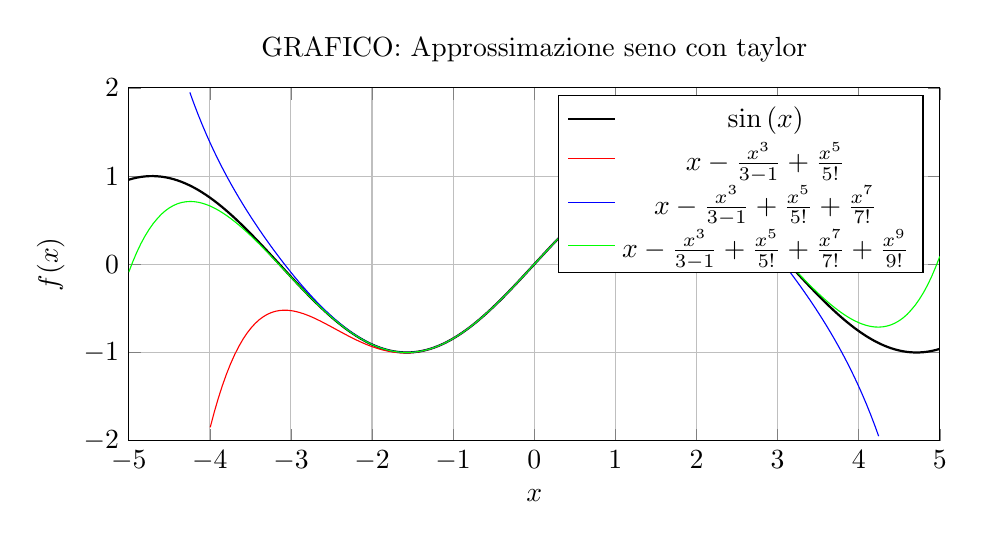
\begin{tikzpicture}
	\begin{axis}[title=GRAFICO: Approssimazione seno con taylor ,
	xmin=-5, xmax=5,
	ymin=-2,ymax=2,
		restrict y to domain = -2:2, domain=-5:5, width=0.98\textwidth, height=0.5\textwidth, grid=major, samples=200,  ylabel=$f(x)$, xlabel=$x$, legend entries={ $\sin \left( x \right) $, $x- \frac{x^3}{3-1} + \frac{x^{5}}{5!}$, $x- \frac{x^3}{3-1} + \frac{x^{5}}{5!} + \frac{x^{7}} {7!}$, $x- \frac{x^3}{3-1} + \frac{x^{5}}{5!} + \frac{x^{7}}{7!}+ \frac{x^{9}}{9!}$}]
		\addplot[black, thick] {sin(deg(x))};
		\addplot[red] {x-(x^3)/6 + (x^5)/5!};
		\addplot[blue] {x-(x^3)/6 + (x^5)/5! - (x^7)/7!};
		\addplot[green] {x-(x^3)/6 + (x^5)/5! - (x^7)/7! + (x^9)/9!};
	\end{axis}
\end{tikzpicture}
\subsection{Sviluppo con Taylor $ \neq 0$}
\label{Taylorno0}
\definizione{Taylor con centro in $x_0$}{
\[
	f\left( x \right) = f\left( x_0 \right) + f'\left( x_0 \right) (x-x_0) + \ldots+ \frac{f^{n}\left( x_0 \right) }{n!}\left( x-x_0 \right) ^{n} + o\left( \left( x-x_0 \right) ^{n} \right) 
\] 
NB: questa formula è equivalente alla formula di Taylor per $ x \to 0$ applicata su una funzione \underline{traslata orizzontalmente verso destra di $x_0$}
}
\incomprensione{10:45:02}
Come cazzo si dimostra?
\begin{itemize}
	\item Calcolando la derivata in $x_0$ ottengo l'approssimazione locale in $ x_0$
	\item Moltiplicando la derivata per $\left( x-x_0 \right) $ traslo il polinomio ottenuto verso destra di $x_0$
\end{itemize}
\section{Teoremi continuoità e derivabilità}
\teorema{Esistenza degli zeri}{
Sia $  f: \left[ a,b \right] \to \R $ una funzione continua. Supponiamo che $  f\left( a \right)  \cdot f\left( b \right)  < 0 $ (ossia che che $ a $ e $ b $ hanno segno discorde). Allora
\[
\exists c \in  \left( a,b \right) \text{ t.c. } f\left( c  \right) =0
\] 
}
NB: posso applicare una variante del teorema. Se $ f : \left[ a,b \right] \to \R $ è continua e $ f\left( a \right) < \lambda  $ e $ f\left( b \right) > \lambda  $ o viceversa, allora
\[
\exists x_0  \text{ t.c. } f\left( x_0 \right) = \lambda 
\] 
Posso generalizzare ulteriormente tramite il teorema dei valori intermedi:
\teorema{Teorema dei valore intermedi}{
Sia $  f: \left( a,b \right) \to \R $ una funzione continua. Sia \[
L = sup \left\{ f\left( x \right) : x \in  \left( a,b \right)  \right\} \text{ e } l = \infty\left\{ f\left( x \right) : x \in  \left( a,b \right)  \right\} 
\] 
Sia $ \lambda   \in  \R$ tale che $ l < \lambda  < L $. Allora 
\[
\exists c \in  \left( a,b \right) \text{ t.c. } f\left( c \right) = \lambda 
\] 
}
Questo equivale a dire che una funzione continua in un intervallo $ \left[ a,b \right]  $ assume tutti i valori compresi fra il suo massimo e il suo minimo. NB: da questo teorema posso ricavare il fatto generale che se:
\[
\lim_{x \to \infty} f(x) = + \infty \text{ e } \lim_{x \to -\infty} f(x) = -\infty
\] 
oppure viceversa, allora $ f\left( x \right)  $ è surgettiva
\subsection{Teoremi studio locale funzione}
\teorema{Criterio di monotonia 1}{
Sia $  f: A \to \R  $ e $ x_0 \in  A $. Supponiamo che $ f'\left( x \right) > 0 $. Allora esiste $ \delta >0 $ tale che:
\begin{itemize}
	\item $ f\left( x \right)  > f\left( x_0 \right) \quad  \forall x \in  \left( x_0 , x_0+ \delta   \right)  $
	\item $ f\left( x \right)  < f\left( x_0 \right) \quad  \forall x \in  \left( x_0- \delta , x_0  \right)  $
\end{itemize}
}
NB: l'affermazione si limita allo studio \underline{locale} di una funzione. La funzione è quindi \underline{crescente} ma \underline{solo localmente}
\definizione{Punto stazionario}{
Sia $ f $ derivabile in $ x_0 $. Se $ f'\left( x_0 \right)  $ allora il punto $ x_0 $ è detto \underline{ punto stazionario}
}
NB: ho 5 possibili punti stazionari:
	\begin{itemize}
		\item Punto di massimo
		\item Punto di minimo
		\item Flesso a tangenza orizzontale ascendente
		\item Flesso a tangenza orizzontale discendente
		\item Funzioni patologiche che oscillano in a fucked-up fashion
	\end{itemize}
Esempio di quest'ultimo caso:
\[
f\left( x \right)  =
\begin{cases}
	x^2 \sin \left( \frac{1}{x} \right) \quad x \neq 0	\\
	0 \quad x=0
\end{cases}
\] 
\begin{center}
	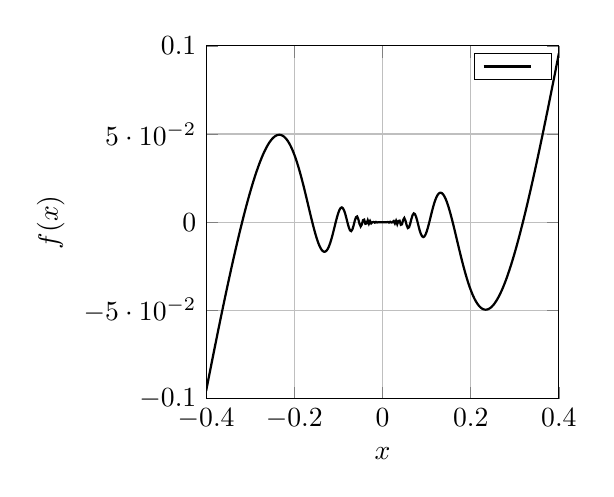
\begin{tikzpicture}
		\begin{axis}[
		xmin=-0.4, xmax=0.4,
		ymin=-0.1,ymax=0.1,
		restrict y to domain = -0.1:0.1, domain=-0.4:0.4, width=0.5\textwidth, height=0.5\textwidth, grid=major, samples=300,  ylabel=$f(x)$, xlabel=$x$, legend entries={$ $}]
		\addplot[black, thick] {x^2*sin(deg(1/x))};
		\end{axis}
	\end{tikzpicture}
\end{center}
Questa funzione oscilla sempre più avvicinandosi all'origine, ma la derivate in 0 esiste ed è nulla
\teorema{Criterio delle derivate successive}{
Immagino di cercare la prima derivata che non si annulla in un punto $ x_0 $. Supponiamo che questa derivata sia di ordine $ k $:
\[
f'\left( x_0 \right) =f''\left( x_0 \right) =f'''\left( x_0 \right)=f^{\left( k-1 \right) }\left( x_0 \right)  =0 
\]
ho 4 opzioni:

\begin{center}
	\begin{forest}
	[k, for tree={forked edges, draw=gray!20, align=left, grow'=0}
		[ è pari 
			[ $ f^{k}(x_0) > 0 $
				[$x_0$ è \underline{minimo locale}]
			]
			[ $ f^{k}(x_0) < 0 $
				[$x_0$ è \underline{minimo locale}]
			]
		]
		[ è dispari 
			[ $ f^{k}(x_0) > 0 $
				[$x_0$ è flesso a tg. orizzontale \underline{ascendente}]
			]
			[ $ f^{k}(x_0) < 0 $
				[$x_0$ è flesso a tg. orizzontale \underline{discendente}]
			]
		]
	]
\end{forest}
\end{center}
}
Dimostrazione: la dimostrazione è interesante e usa lo sviluppo di Taylor
\begin{itemize}
	\item Calcolo sviluppo di Taylor in $  x_0 $ in modo tale da approssimare concavità della funzione (vedi \textit{sezione \ref{Taylorno0}})
	\[
	f\left( x \right) = f\left( x_0 \right)  + f'\left( x_0 \right) \left( x-x_0 \right) +\ldots+ \frac{f^{k}\left( x_0 \right)}{k!}\left( x-x_0 \right) ^{k} + o\left( \left( x-x_0 \right) ^{k} \right)  \quad \text{ per } x \to x_0
	\] 
	\item Per un valore di $ h $ molto piccolo posso calcolare il polinomio in $ x_0+h $, visto che non mi distaccherei troppo dall'intorno in cui il polinomio è approssimato bene:
	\[
	f\left( x_0+h \right) = f\left( x_0 \right) + f'\left( x_0 \right) h + \ldots + \frac{f^{k}\left( x_0 \right)}{k!}h^{k} + o \left( h^{k} \right)  
	\] 
	\item Noto che per ipotesi le derivate di ordine $ 1,\ldots,k-1 $ sono tutte nulle, quindi lo sviluppo di Taylor è il seguente:
	\[
	f\left( x_0+h \right) = \frac{f^{k}\left( x_0 \right)}{k!}h^{k}+ o\left( h^{k} \right)  
	\] 
	\item Dividendo per $ h^{k} $ elimino l'o-piccolo per definizione e ottengo:
	\[
	\frac{f\left( x_0+h \right)- f\left( x_0 \right) }{h^{k}}= \frac{f^{\left( k \right) }\left( x_0 \right) }{k!}
	\] 
	\item Noto che ho a destra la derivata \textit{k-esima} di $ f $. Riprendendo le affermazioni riguardo segno della derivata e parità di $ k $ posso osservare che, ad esempio, se $ f\left( x_0 +h\right)  > f\left( x_0 \right) $ $ x_0 $ è un punto di minimo locale. Le stesse affermazioni si possono fare per i flessi e i massimi
	\end{itemize}

\teorema{Teorema di Weierstrass}{
Sia $f : \left[ a,b \right] $ una funzione continua nell'intervallo $\left[ a,b \right] $. Allora esistono almeno un massimo e un minimo assoluto in $\left[ a,b \right] $
}
Varianti Weierstrass:
\begin{itemize}
	\item Sia $  f: \R \to \R $ continua e \underline{periodica}. Allora esistono MAX e MIN
	\item Sia $  f: \R \to \R $ continua. Supponiamo che 
	\[
	\lim_{x \to +\infty} f(x) = \lim_{x \to -\infty} f(x) = \pm \infty
	\] 
	allora esiste MIN/MAX (rispettivamente per $ +\infty/-\infty $)
\end{itemize}

\teorema{Teorema di Rolle}{
Sian $f: \left[ a,b \right]  \to \R$. Supponiamo che 
\begin{itemize}
	\item $f$ è continua in $\left[ a,b \right] $
	\item $f$ è derivabile in $ \left( a,b \right) $
	\item $f\left( a \right) = f\left( b \right) $
\end{itemize}
allora 
\[
\exists x_0 \in  \left( a,b \right) \text{ t.c. } f'\left( x_0 \right) =0
\] 
}
\teorema{Teorema di Cauchy}{
Siano $f:\left[ a,b \right] \to \R, \quad  g:\left[ a,b \right] \to \R$. Supponiamo che 
\begin{itemize}
	\item $f$ e $g$ sono continue in $\left[ a,b \right] $
	\item $f$ e $g$ sono derivabili in $ \left( a,b \right) $
\end{itemize}
Allora $\exists x_0 \in  \left( a,b \right)$  tale che 
\[
\left( f\left( b \right) - f\left( a \right)  \right) g'\left( x_0 \right) = \left( g\left( x \right) -g\left( a \right)  \right) f_0\left( x_0 \right) 
\] 
se inoltre 
\begin{itemize}
	\item  $g'\left( x \right) \neq 0 \quad \forall x \in \left( a,b \right) $
\end{itemize}
allora $g\left( b \right) \neq g\left( a \right) $ e dividendo per $g_0\left( x_0 \right) $ ottengo
\[
\frac{f\left( b \right) - f\left( a \right) }{g\left( b \right) -g\left( a \right) }= \frac{f'\left( x_0 \right)}{g'\left( x_0 \right) } 
\] 
}
NB: se penso a teorema di Lagrange, noto che il rapporto fra le derivate è esattamente il rapporto fra i $ \Delta  y$ che la funzione assume agli estremi:
\[
f'\left( x_0 \right) = \frac{f\left( b \right) -f\left( a \right)}{b-a} \quad g'\left( x_0 \right) = \frac{g\left( b \right) - g\left( a \right) }{b-a}
\] 
Facendo il rapporto $  b-a $ si annulla e ottengo esattamente quanto espresso da teorema di Cauchy
\vskip3mm
Dimostrazione:
\begin{itemize}
	\item Uso rolle su una nuova funzione definita nel seguente modo:
	\[
	\phi \left( x \right) = \left( f\left( b \right) -f\left( a \right)  \right) g\left( x \right) - \left( g\left( b \right) -g\left( a \right)  \right) f\left( x \right) 
	\] 
	\item Noto che 
	\begin{itemize}
		\item $\phi $ è continua in $\left[ a,b \right] $ in quanto \textit{combinazione lineare }di funzioni derivabili
		\item $\phi $ è derivabile in $ \left( a,b \right) $ in quanto \textit{combinazione lineare }di funzioni derivabili
		\item $\phi\left( a \right) = \phi \left( b \right)  $. Basta verificare inserendo $a$ e $b$
	\end{itemize}
\item La funzione soddisma le ipotesi del \underline{teorema di Rolle} ossia:
\[
	\phi' \left( x \right) = \left( f\left( b \right) -f\left( a \right)  \right) g'\left( x \right) - \left( g\left( b \right) -g\left( a \right)  \right) f'\left( x \right) =0
\] 
ottengo quindi l'ipotesi 1 del teorema
\end{itemize}
\teorema{Teorema di Lagrange}{
Sia $f:\left[ a,b \right] \to \R$. Supponiamo che 
\begin{itemize}
	\item f è continua in  $\left[ a,b \right] $
	\item f è derivabile in $\left( a,b \right) $
\end{itemize}
Allora $\exists x_0 \in  \left( a,b \right) \text{ t.c. }$ 
\[
f\left( b \right) - f\left( a \right) = f'\left( x_0 \right) \left( b-a \right) 
\] 
}
Dimostrazione:
\begin{itemize}
	\item Uso teorema di Cauchy con $g\left( x \right) =x$
	\[
	\frac{f\left( b \right) -f\left( a \right) }{b-a}=f'\left( x_0 \right) 
	\] 
\end{itemize}
\teorema{Teorema monotonia 2}{
Sia $f:\left[ a,b \right] \to \R$. Supponiamo
\begin{itemize}
	\item $f$ continuo in $\left[ a,b \right] $
	\item $f$ derivabile in $\left( a,b \right) $
\end{itemize}
allora
\begin{itemize}
	\item Se $ f'\left( x \right) > 0 \quad \forall x \in  \left( a,b \right) \Rightarrow f$ è strettamente crescente
	\item Se $f'\left( x \right) \ge 0 \quad \forall x \in  \left( a,b \right) \Rightarrow f$ è debolmente crescente
	\item Se $f$ è strettamente crescente allora $ f_0\left( x \right)  \ge 0 \quad  \forall x \in  \left( a,b \right) $
	\item Se $f$ è debolmente crescente allora $ f_0\left( x \right) \ge 0 \quad \forall x \in  \left( a,b \right) $
\end{itemize}
}
Dimostrazione:
\begin{itemize}
	\item Per ipotesi $f$ è debolmente crescente. Prendo $x_0 \in  \left( a,b \right) $ 
	\[
	f'\left( x_0 \right) = \lim_{h \to 0^{+}} \frac{f\left( x_0+h \right) -f\left( x_0 \right)}{h}  
	\] 
	\item Se $f$ è crescente allora il denominatore del rapporto incrementale è \underline{positivo}. Il limite per $h \to o^{+}$ è quindi positivo.
\end{itemize}
\hr
\begin{itemize}
	\item Per ipotesi $f_0\left( x \right) > 0 \quad  \forall x \in  \left( a,b \right) $
	\item Applico Lagrande a $\left[ c,d \right] \subseteq \left[ a,b \right] $ e ottengo:
	\[
	f\left( d \right) - f\left( c \right) =f'\left( x_0 \right) \left( d-c \right) 
	\] 
	\item Siccome $f'\left( x \right) > 0$ per ipotesi e $\left( d-c \right) > 0$ allora $f\left( d \right) -f\left( c \right) > 0$
	\item Vista l'arbitrarietà nella scelta di $d$ e $c$ posso affermare che $f$ è crescente
\end{itemize}
\teorema{Teorema monotonia 3}{
Sia $f:\left[ a,b \right] \to \R$. Supponiamo che 
\begin{itemize}
	\item $f$ è continua in $\left[ a,b \right] $
	\item $f$ è derivabile in $ \left( a,b \right) $
	\item $f'\left( x \right)  \ge 0 \quad \forall x \in  \left( a,b \right) $
	\item Non esiste alcun intervallo contenuto in $\left( a,b \right) $ in cui $f'$ è sempre $=0$. E' possibile tuttavia che $f'\left( x \right) =0$ in punti isolati (\textit{sporadicamente})
\end{itemize}
allora
\[
f \text{ è strettamente crescente in } \left( a,b \right) 
\] 
}
Dimostrazione:
\begin{itemize}
	\item Per ipotesi $f$ è debolmente crescente: se non fosse strettamente crescente vorrebbe dire che c'è un intervallo in cui $f$ è costante. Questo però viola la condizione 4 per cui $f$ è strettamente crescente
\end{itemize}
\definizione{Lipschizzianità}{
Sia $ A \in  \R$ e sia $ f: A \to \R$. si dice che $f$ è lipschizziana in $A$ se esiste $L \in  \R$ tale che $ \forall x, y \in  A$ si ha
\[
	\left|f\left( x \right)  - f\left( y \right) \right| \le L \left| x-y\right|
\] 
}
Esempi:

\begin{minipage}[t]{0.48\textwidth}
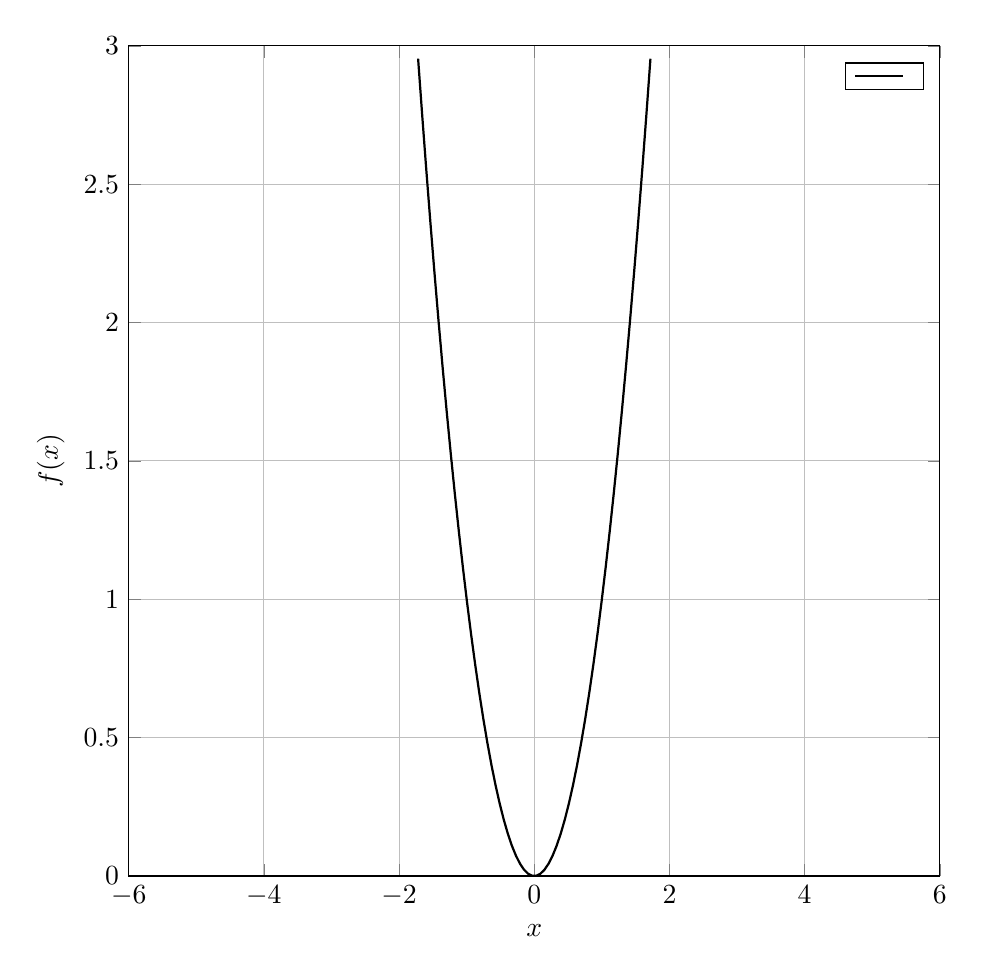
\begin{tikzpicture}
	\begin{axis}[xmin=-6, xmax=6,
	ymin=0,ymax=3,
	restrict y to domain = 0:3, domain=-6:6, width=0.98\textwidth, height=\textwidth, grid=major, samples=200,  ylabel=$f(x)$, xlabel=$x$, legend entries={$ $}]
	\addplot[black, thick] {x^2};
	\end{axis}
\end{tikzpicture}
	No, se $x \to \infty$ la pendenza è infinita. Sì se considero intervallo $\left[ -1,1 \right] $
\end{minipage}
%
\begin{minipage}[t]{0.48\textwidth}
\begin{tikzpicture}
	\begin{axis}[xmin=-6, xmax=6,
	ymin=0,ymax=8,
	restrict y to domain = 0:3, domain=-6:6, width=0.98\textwidth, height=\textwidth, grid=major, samples=200,  ylabel=$f(x)$, xlabel=$x$, legend entries={$ $}]
		\addplot[black, thick] {sqrt(x)};
	\end{axis}
\end{tikzpicture}
	No, se $x \to 0$ la pensenza è infinita. Si se considero intervallo $[1, + \infty)$
\end{minipage}
\teorema{Continuità e lipschizianità}{
Sia $ f A \to \R$ lipschizziana. Allora
\[
f \text{ continua in } A
\] 
}
\teorema{Continuità e lipschizianità 2}{
Sia  $ F: A \to \R$ con $A$ \underline{convesso}. Allora 
\[
	f \text{ è lipschizziana in }A \Leftrightarrow \left|f'\left( x \right) \right| \text{ è limitato }
\] 
in più, in quest'ultimo caso si ha che 
\[
	L = sup\left( \left|f'\left( x \right) \right| : x \in  \left[ 0,1 \right]   \right) 
\] 
}
NB: 
\textbox{
Posso sfruttare quest'ultimo teorema per ottenere importanti disuguaglianze. 
}
Se trovo la minima costante di lipschiz posso applicare la definizione per ottenere la disuguaglianza


\subsection{Proprietà sviluppi taylor}
\subsubsection{Somma}
Dati due due sviluppi di taylor
\[
	f\left( x \right) = P_1\left( x \right)  + o\left( x^{n} \right) \quad g\left( x \right) = P_2\left( x \right)  + o\left( x^{n} \right)
\]
allora lo sviluppo della somma di $f\left( x \right) $ e $g\left( x \right) $ è
\[
	P_1\left( x \right)  + P_2\left( x \right) + o\left( x^{n} \right)
\]
\subsubsection{Prodotto}
Dati due due sviluppi di taylor
\[
	f\left( x \right) = P_1\left( x \right)  + o\left( x^{n} \right) \quad g\left( x \right) = P_2\left( x \right)  + o\left( x^{n} \right)
\]
allora lo sviluppo del prodotto di $f\left( x \right) $ e $g\left( x \right) $ è
\[
	P_1\left( x \right)  \cdot P_2\left( x \right) + o\left( x^{n} \right)
\]
NB: quando si moltiplica $P_1$ con $P_2$ tutti i termini di grado $ >n$ vengono inglobati all'interno di $o\left( x^{n} \right) $, non serve quindi calcolarli
\subsection{Composta}
Dati due due sviluppi di taylor
\[
	f\left( x \right) = P_1\left( x \right)  + o\left( x^{n} \right) \quad g\left( x \right) = P_2\left( x \right)  + o\left( x^{n} \right)
\]
allora lo sviluppo della funzione composta $f\left( g\left( x \right)  \right) $
\[
	P_1\left( x \right)  \cdot P_2\left( x \right) + o\left( x^{n} \right)
\]
\subsubsection{Esempi di sviluppi}
\textbf{Esempio 1}
\[
	\cos x + 2 \sin x
\]
\begin{align*}
	\cos x            & =  1-\frac{x^2}{2}+\frac{x^{4}}{24} + o\left( x^{4} \right)                           \\
	\sin x            & =  x - \frac{x^3}{6} + o \left( x^{4} \right)                                         \\
	\cos x + 2 \sin x & =  1 - \frac{x^2}{2} + \frac{x^{4}}{24} + 2x - \frac{x^3}{3} + o \left( x^{4} \right) \\
	                  & = 1 + 2x - \frac{x^2}{2} - \frac{x^3}{3} + \frac{x^{4}}{ 24} + o\left( x^{4} \right)
\end{align*}
\textbf{Esempio 2}
\[
	\arctan x + \sinh x
\]
\begin{align*}
	\arctan x \cdot \sinh x & = \left( x- \frac{x^3}{2} + \frac{x^{5}}{5} + o\left( x^{5} \right)  \right) \left( x + \frac{x^3}{6} + \frac{x^{5}}{120} + o \left( x^{5} \right)  \right) \\
	                        & = x^2 - \frac{1}{6}x^{4} + o\left( x^{5} \right)
\end{align*}
NB: se venisse chiesto (come è purtroppo già accaduto) di dire quanto vale, ad esempio $f^{\left( 4 \right) }\left( 0 \right) $ non è conveniente derivare, ci si incasina. Bisogna invece
\begin{itemize}
	\item Calcolare lo sviluppo di Taylor con $n=4$
	\item Realizzare che il coefficiente del termine di grado 4 è uguale a $\frac{f^{\left( 4 \right) }\left( 0 \right)}{4!} $
\end{itemize}

\section{Convessità}
\begin{definizione}{Convessità/concavità sottoinsiemi}
	Un sottoinsieme $ A \subseteq \R$ si dice \underline{convesso }se per ogni coppia di punti $x,y \in  A$ allora
	\[
		\left[ x,y \right] \subseteq A
	\]

\end{definizione}
NB: ciò accade per 3 tipi di insieme:
\begin{itemize}
	\item $A \cong \R$
	\item Ogni semiretta: $\left( -\infty, a \right) \quad (-\infty, a ]  \quad [a, + \infty) \quad \left( a,+ \infty \right) $
	\item Gli intervalli: $\left( a,b \right) \quad [a,b) \quad (a, b] \quad \left[ a,b \right] $
\end{itemize}

\begin{definizione}{Convessità geometrica}
	Sia $A \subseteq  \R$ convesso. Una funzione $f : A \to \R$ si dice \underline{ convessa }se per ogni coppia di punto $P, Q$ nel grafico di $f$ tutto il segmento $PQ$ sta sopra il grafico

\end{definizione}

\begin{definizione}{Convessità algebrica}
	Sia $A \subseteq \R$. Una funzione $f: A \to \R$ si dice convesso se $ \forall a,b \in  A \quad \forall \lambda \in \left[ 0,1 \right] $
	\[
		f\left( \lambda  a + \left( 1-\lambda  \right) b \right) \le \lambda f\left( a \right)  + \left( 1-\lambda  \right) f\left( b \right)
	\]

\end{definizione}
Interpretazione geometrica:
\begin{itemize}
	\item la quantità $\lambda a + \left( 1- \lambda  \right) b$ con $ \lambda  \in  \left[ 0,1 \right] $ posso esprimere ogni punto compreso fra  $a$ e $b$ :
	      \begin{itemize}
		      \item $\lambda  = \frac{1}{2} \quad \rightarrow \quad \frac{a+b}{2}$
		      \item $\lambda  = 1 \quad \rightarrow a$
		      \item $\lambda  = 0 \quad \rightarrow b$
	      \end{itemize}
	\item
	\item Allo stesso modo la quantià $\lambda f\left( a \right)  + \left( 1-\lambda  \right) f\left( b \right)$ esprime un punto compreso fra $f\left( a \right) $ e $f\left( b \right) $
	\item Per ogni valore di $\lambda $ ottengo a sinistra $f\left( c \right) $ mentre a destra ottengo $g\left( c \right) $ dove g è la retta passante per $a\left( f\left( a \right)  \right) , \left( b,f\left( b \right)  \right)  $ con $c \in  \left[ a,b \right] $
\end{itemize}
\subsection{Convessità e derivata}
Sia $ A \subseteq  \R$ convesso e sia $ f: A \to \R$. Sappiamo che $f''\left( x \right) $ esiste $ \forall x \in  A$. Posso affermare con certezza che:
\begin{itemize}
	\item se $f''\left( x \right)  > 0 \forall x \in  A \rightarrow f$ è strettamente crescente
	\item se $f''\left( x \right)  \ge 0 \forall x \in  A \rightarrow f$ è debolmente crescente
	\item $f$ è debolmente crescente $ \Rightarrow f''\left( x \right) \ge 0 \forall  x \in A$
\end{itemize}
NB: è falso affermare che
\begin{itemize}
	\item se $f$ è strettamente crescente $ \Rightarrow f''\left( x \right) > 0 $
\end{itemize}
basti pensare alla funzione $x^4$.Pur essento \underline{strettamente concava} la sua derivata si annulla in 0
\section{Teoria di integrazione}
\subsection{Come si indicano}
\[
	\int_{a}^{b} f\left( x \right)  \; dx
\]
\begin{itemize}
	\item $\left[ a,b \right] $ zona di integrazione, cioè l'insieme in cui integriamo
	\item $f: \left[ a,b \right] $ la funzione che si integra (integranda)
	\item $dx$ simbolo che indica la variabile di integrazione
	\item la funzione $f$ è liminata in $\left[ a,b \right] $
\end{itemize}
\subsection{Significato geometrico}
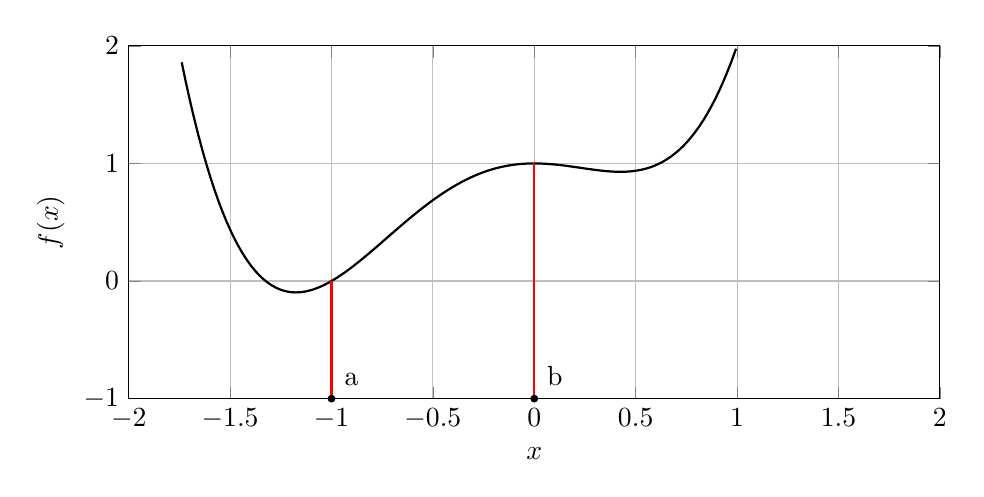
\begin{tikzpicture}
	\begin{axis}[
			xmin=-2, xmax=2,
			ymin=-1,ymax=2,
			restrict y to domain = -1:2, domain=-2:2, width=0.98\textwidth, height=0.5\textwidth, grid=major, samples=200,  ylabel=$f(x)$, xlabel=$x$]
		\addplot[black, thick] {x^3 - x^2+ x^4+1};
		\draw [red, thick] (-1,0) to (-1,-1);
		\draw [red, thick] (0,1) to (0,-1);
		\coordinate (p1) at (0,-1);
		\coordinate (p2) at (-1,-1);
	\end{axis}
	\node [label=45: a , fill=black, circle, inner sep = 1pt] at (p2) {};
	\node [label=45: b , fill=black, circle, inner sep = 1pt] at (p1) {};
\end{tikzpicture}
Come in figura, l'integrale rappresenta l'area sottesa al grafico della funzione fra $ a $ e $ b $. In questo caso è:
\[
	\int_{a}^{b} f\left( x \right)  \; dx
\]
\subsection{Definizione formale}
\begin{itemize}
	\item Caso banale \rarr funzioni costanti
	\item Caso semi-banale \rarr funzioni a gradino
	\item Caso generale
\end{itemize}
\textbf{Caso 1:}
\[
	f\left( x \right)  = \lambda \in  \R \quad \quad \forall x \in  \left[ a,b \right]
\]
In questo caso l'area è chiaramente l'area del rettangolo contenuto sotto $f\left( x \right) $
\[
	\int_{a}^{b} f\left( x \right)  \; dx = \left( b-a \right) \lambda
\]
\textbf{Caso 2:}
\[
	\text{ La funzione è costante su determinati sotto intervalli di } \left[ a,b \right]
\]
L'area in questo caso è chiaramente la somma dell'area di ogni rettangolo creato da ogni sotto intervallo costante di $ f\left( x \right) $
\[
	\int_{a}^{b} f\left( x \right)  \; dx = \sum_{k=1}^{n} \left( b-a \right) \lambda_k
\]
\textbf{Caso 3}
\[
	\text{ La funzione non è ne costante ne a scalini ma \underline{limitata} }
\]
In questo caso procedo nel seguente modo:
\begin{itemize}
	\item Provo ad approssimare l'area del grafico sotteso alla funzione tramite funzione a scalini
	\item Considero rispettivamente la funzione a gradini che stima l'area \underline{dal sopra} e \underline{dal sotto}
	\item Sia $ f : \left[ a,b \right] \to \R$ limitata. Si dice \underline{integrale superiore di $f$ in $\left[ a,b \right] $}
	      \[
		      I^{+}\left( f, \left[ a,b \right]  \right) = inf \left\{ \int_{a}^{b} p\left( x \right)   \; dx : p:\left[ a,b \right] \to \R \text{ f. a gradino t.c. } p\left( x \right) \ge f\left( x \right)  \right\}
	      \]
	      Analogamente si definisce l'integrale inferiore:
	      \[
		      I^{-}\left( f, \left[ a,b \right]  \right) = sup \left\{ \int_{a}^{b} p\left( x \right)   \; dx : p:\left[ a,b \right] \to \R \text{ f. a gradino t.c. } p\left( x \right) \le f\left( x \right)  \right\}
	      \]
	      Fatto generale molto intuitivo:
	      \[
		      I^{+}\left( f, \left[ a,b \right]  \right) \ge I^{-} \left( f, \left[ a,b \right]  \right)
	      \]
	\item Se accade che $ I^{+}\left( f, \left[ a,b \right]  \right) = I^{-} \left( f, \left[ a,b \right]  \right)  $ allora si dice che $f:  \left[ a,b \right] \to \R$ è \underline{integrabile} su $ \left[ a,b \right] $ e il valore ottenuto si indica con in simbolo
	      \[
		      \int_{a}^{b} f\left( x \right)  \; dx
	      \]
\end{itemize}
\subsection{Teoremi integrabilità}
\begin{teorema}{Integritabilità funzione}
	I seguenti tipi di funzione sono integrabili:
	\begin{itemize}
		\item Tutte le funzioni \underline{monotone} (anche non continue)
		\item Tutte le funzioni \underline{continue}
		\item Tutte le funzione che hanno un numero finito di punti di discontinuità nei quali i limini destro e sinistro esistono
	\end{itemize}
\end{teorema}

Dimostrazione per funzioni monotone:
\begin{itemize}
	\item Se per un dato $\epsilon < 0 $ trovo una somma di Riemann superiore e una inferiore la cui differenza è $ < \epsilon $ sono a cavallo
	\item Divido il grafico di  $f\left( x \right) $ in $n$ parti uguali e creo somma di Riemann dall'alto:
	      \begin{itemize}
		      \item La somma di Riemann superiore prenderà come altezza di ogni intervallo il valore della funzione di destra
		      \item La somma di Riemann inferiore prenderà come altezza di ogni intervallo il valore della funzione di sinistra
	      \end{itemize}
\end{itemize}

\begin{center}
	\input{Images/Riemann.pdf_tex}
\end{center}

\subsection{Proprietà integrali}
\[
	\begin{lgathered}
		\int_{a}^{b} \left( f\left( x \right) + g\left( x \right)  \right)  \; dx =  \int_{a}^{b} f\left( x \right)  \; dx + \int_{a}^{b} g\left( x \right)  \; dx\\
		\int_{a}^{b} \lambda f\left( x \right)  \; dx =  \lambda \int_{a }^{b} f\left( x \right)  \; dx\\
		\left|\int_{a}^{b} f\left( x \right)  \; dx\right| \le \int_{a}^{b} \left|f\left( x \right) \right|  \; dx\\
		\int_{a}^{b} f\left( x \right)  \; dx = \int_{a}^{c} f\left( x \right)  \; dx + \int_{c}^{b} f\left( x \right)  \; dx \text{ con } c \in  \left[ a,b \right] \\
		\text{ Se } f\left( x \right)  \ge g\left( x \right) \forall x \in  \left[ a,b \right]  \text{ allora }  \int_{a}^{b} f\left( x \right)  \; dx \ge \int_{a}^{b} g\left( x \right)  \; dx\\
	\end{lgathered}
\]
\section{Calcolo di integrali e integrazione impropria}
\subsection{Teoremi e definizioni}
\begin{definizione}{Primitiva di una funzione}
	Sia $ f: \left[ a,b \right]  \to \R $ continua. Si dice \underline{primitiva} di $f$ una qualunque funzione $ F: \left[ a,b \right] \to \R$ tale che $F$ è derivabile in $ \left[ a,b \right] $ e vale
	\[
		F'\left( x \right) = f\left( x \right) \quad  \forall x \in  \left[ a,b \right]
	\]

\end{definizione}

\begin{definizione}{Funzione integrale}
	Sia $ f: \left[ a,b \right] \to \R$ continua. Si dife funzione integrale la funzione:
	\[
		\Phi \left( x \right)  = \int_{a}^{x} f\left( t \right)  \; dt
	\]

\end{definizione}
NB: la funzione integrale gode delle seguenti proprietà:
\[
	\begin{lgathered}
		\int_{a}^{b} f\left( x \right)  \; dx = \Phi \left( b \right) = \left[ \Phi \left( x \right)  \right] _a ^b\\
		\int_{c}^{d} f\left( x \right)  \; dx = \Phi \left( d \right) - \Phi \left( c \right)
	\end{lgathered}
\]
\begin{teorema}{Teorema della media integrale}
	Sia $ f: \left[ a,b \right] \to \R $ continua. Allora esiste almeno un punto $c \in  \left[ a,b \right] $ tale che:
	\[
		\int_{a}^{b} f\left( x \right)  \; dx = f\left( c \right) \left( b-a \right)
	\]
\end{teorema}

\begin{teorema}{Teorema fondamentale del calcolo integrale}
	Sia $ f: \left[ a,b \right] \to \R $  continua. Sia $  \Phi  $ la sua funzione integrale. Allora
	\[
		\Phi ' \left( x \right)  = f\left( x \right) \quad \forall x \in  \left[ a,b \right]
	\]
	ossia $ \Phi  $ è primitiva di $ f $
\end{teorema}

Dimostrazione:
\begin{itemize}
	\item Calcolo il rapporto incrementale di $  \Phi  $ per $ h > 0  $
	      \[
		      \frac{\Phi \left( x+h \right) - \Phi \left( x \right) }{h}= \frac{1}{h}\left[ \int_{x}^{x+h} f\left( t \right) dt \; dt - \int_{a}^{x} f\left( t \right)  \; dt \right]
	      \]
	\item Noto che per addizione di integrali posso riscrivere il membro di destra come
	      \[
		      \frac{1}{h} \int_{x}^{x+h} f(t) \; dt
	      \]
	\item Per il teorema dei valori intermedi so che esiste un punto $ \in \left[ x, x+h \right]  $ tale che $  f\left( c \right) = \int_{x}^{x+h} f\left( x \right)  \; dx$ quindi:
	      \[
		      \frac{1}{h} \cdot h \cdot f\left( c \right)
	      \]
	\item Noto che se $ h \to 0 $ allora $  c \to x $, per cui $ f\left( c \right) \to f\left( x \right)  $. Questa affermazione posso farla in quanto $  f\left( x \right)  $ è \underline{continua}
	\item Se applico il limite per $ h \to 0 $ al rapporto incrementale ottengo che
	      \[
		      \Phi '\left( x \right) = \lim_{h \to 0} \frac{\Phi \left( x+h \right) -\Phi \left( x \right) }{h} = \lim_{h \to 0} f\left( c \right) = f\left( x \right)
	      \]
	      ho quindi dimostrato che $ \Phi  $ è derivabile e che $ \Phi '\left( x \right)  = f\left( x \right) $ ossia che $ \Phi  $ è una primitiva di $ f $
\end{itemize}
\subsection{Integrazione di funzioni razionali}
Una funzione razionale è una funzione del tipo
\[
	\frac{P\left( x \right) }{q\left( x \right) }
\]
Per integrare una cosa di questo tipo devo seguire 4 passaggi:
\begin{itemize}
	\item Divisione
	\item Fattorizzazione del denominatore
	\item Risolvere sistema lineare
	\item Integrazione
\end{itemize}
\subsubsection*{Divisione} Se il grado di $ P $ è $ < $ del grado di $ Q $ si passa al punto 2, altrimenti divido $ P\left( x \right)  $ per $  Q\left( x \right)  $ ottenendo:
\[
	\frac{P\left( x \right) }{Q\left( x \right) }= A\left( x \right) + \frac{R\left( x \right) }{P\left( x \right) }
\]
nota che avendo diviso, la funzione $ \frac{R\left( x \right)}{P\left( x \right) }  $ ha il grado del numeratore $ < $ del grado del denominatore
\vskip3mm
\textbf{Fattorizzazione:} Scomporre il numeratore in prodotto di polinomi di primo e secondo grado con i termini di secondo grado che non sono ulteriormente scomponibili. Esempio bello:
\[
	x^{4} + 1 = x^{4} + 1 + 2x^2 - 2x^2= \left( x^2 + 1 \right)^{2}- \left( \sqrt{2} x \right) ^2 = \left( x^2 + 1 + \sqrt{2} x \right) \left( x^2 + 1 - \sqrt{2} x \right)
\]
\subsubsection*{Fattorizzazione e sistema lineare}
L'obbiettivo è riscrivere la funzione razionale come somma di funzioni razionali. In generale posso avere i seguenti casi:
\begin{itemize}
	\item Al denominatore ho solo termini di grado 1. La somma sarà del tipo
	      \[
		      \frac{A}{P_1\left( x \right) }+ \frac{B}{P_2\left( x \right) }
	      \]
	\item Al denominatore ho dei termini di grado 2 non scomponibili. In questo caso, al di sopra di questi termini dovro avere un polinomio generico di grado 1:
	      \[
		      \frac{A}{P_1\left( x \right) }  + \frac{Bx + C}{P_2\left( x \right) }
	      \]
	\item Se ho fattori con molteplicità $ >1 $ devo seguire un metodo particolare spiegato dopo. In generale, ottengo qualcosa del tipo:
	      \[
		      \frac{A}{P_1\left( x \right) }+ \frac{Bx + C}{P_2\left( x \right) } + \frac{d}{dx}\left[ \frac{Fx^{n-1}\ldots  + Mx + N}{\left( P_1\left( x \right)  \right) ^{2}\left( P_2\left( x \right)  \right) ^{3}} \right]
	      \]
\end{itemize}
\hr
\subsubsection*{Esempio caso 1}
\[
	\frac{P\left( x \right) }{Q\left( x \right) }= \frac{x}{x^2-1}= \frac{x}{\left( x-1 \right) \left( x+1 \right) }= \frac{A}{x-1}+ \frac{B}{x+1}
\]
Devo cercare $ A $ e $ B $ in modo tale che venga soddisfatta l'uguaglianza fra i numeratori dei polinomi:
\[
	x=A\left( x+1 \right) +B\left( x-1 \right)
\]
Svolgo i conti a destra e raccolgo:
\[
	A\left( x+1 \right) +B\left( x-1 \right)= Ax + A + Bx - B = \left( A+B \right) x + A - B
\]
quindi ottengo il seguente sistema lineare eguagliando i coefficienti:
\[
	\begin{cases}
		A+B = 1 \\
		A-B = 0
	\end{cases}
	\rightarrow A = \frac{1}{2} \quad B = \frac{1}{2}
\]
\hr
\subsubsection*{Esempio caso 2}
Se al denominatore ho fattori di grado $ \neq 1$, dovrò trovare il valore di 3 costanti $ A, B, C $. Es:
\[
	\frac{2x^2 + 3}{x^3 - 1}= \frac{A}{x-1} + \frac{Bx + C}{x^2 + x +1}
\]
eseguendo i conti e raccogliendo:
\[
	\frac{\left( A + B \right) x^2 + \left( A- B + C \right) x + A - C}{\left( x-1 \right) \left( x^2 + x+1 \right) }
\]
e ottengo il sistema lineare a 3 incognite:
\[
	\begin{cases}
		A + B = 2    \\
		A - B + C =0 \\
		A - C = 3
	\end{cases}
	\rightarrow A= \frac{5}{3} \quad B = \frac{1}{3} \quad C = - \frac{4}{3}
\]
Quindi, in generale, dove al denominatore ho un polinomio di grado 1 sopra avrò una costante, mentre se al denominatore ho un polinomio di grado 2, al numeratore ho un polinomio generico di grado 1:
\[
	\frac{x^3 + 5}{\left( 2x + 1 \right) \left( x-3 \right) \left( x-8 \right) \left( x^2+1 \right) \left( x^2 + x +1 \right) }
\]
\[
	\frac{A}{2x+1} + \frac{B}{x-1} + \frac{C}{x-8} + \frac{Dx + E}{x^2+1}+\frac{Fx + G}{x^2 + x +1}
\]
quindi ottengo un sistema in tante incognite quanto è il \underline{grado del denominatore}
\hr
\subsubsection*{Esempio caso 3}
Se i fattori al denominatore hanno molteplicità $ > 1$ procedo nel seguente modo:
\begin{multline*}
	\frac{P\left( x \right) }{\left( x+1 \right) ^{4} \left( x+5 \right) ^2\left( x+7 \right) \left( x^2 +1 \right) ^3} =\frac{A}{x+1} + \frac{B}{x+5} + \frac{C}{x+7}+ \frac{Dx + E}{x^2+1} \\ + \frac{d}{dx}\left[ \frac{F x ^{7 }+ G x ^{6} + H x^{5}+ J x^{4}+ K x^3 + L x^2 + Mx + N}{\left( x+1 \right) ^3 \left( x+5 \right) \left( x^2 + 1 \right) ^2} \right]
\end{multline*}
Ossia:
\begin{itemize}
	\item Scrivo fattorizzazione del denominatore e la scrivo come somma, \underline{ignorando la molteplicità} di ogni termine (occhio però a non trascurare il fatto che al numeratore del termini di secondo grado andrà un polinomio di primo)
	\item A questo aggiungo la derivata di un polinomio in cui ho:
	      \begin{itemize}
		      \item \underline{Al denominatore} il prodotto dei polinomi che avevo originariamente al denominatore \underline{abbassati di un grado}
		      \item \underline{Al numeratore} la somma di $ n-1 $ polinomi generici di grado $ 0,\ldots, n-1 $ dove $ n $ è il grado del denominatore
	      \end{itemize}
\end{itemize}
\subsubsection*{Integrazione}
Svolti i passaggi spiegati precedentemente posso ritrovarmi 3 tipi di funzioni da integrare:
\begin{itemize}
	\item Funzioni del tipo $ \displaystyle \frac{k}{ax + c} $, integrate, diventano semplici logaritmi
	\item Funzioni del tipo $ \displaystyle \frac{P_1\left( x \right) }{P_2\left( x \right) } $ dove $ p_1 $ è di grado 1 e $ P_2 $ è grado 2 \underline{non scomponibile}, integrate, diventano arcotangenti. Devo usare completamento del quadrato al denominatore
\end{itemize}

\subsection{Trucchetti integrazione}
\subsubsection*{Integrazione radici di polinomi di secondo grado}
\[
	\boxed{\int \sqrt{1-x^2}}
\]
Metodo trigonometrico
\begin{itemize}
	\item Sostituzione $ x=\sin \left( y \right)  $
	\item Uso formule trigonometriche tenendo conto che $ 1-\sin ^2 \left( y \right) = \cos ^2 y $
\end{itemize}
Metodo della sostituzione
\begin{itemize}
	\item Scrivo come somma per differenza
	\item Sostuisco l'intera radice con uno dei due termini $ =y $ e l'altro rimane invariato. Es $ \sqrt{x^2 -1} =\sqrt{\left( x+1 \right) \left( x-1 \right) } = y\left( x-1 \right)  $
	      i
\end{itemize}
Più in generale, se ho un polinomio con due radici reali $ \lambda, \rho   $, allora posso applicare la sostituzione:
\[
	\sqrt{ \text{ polinomio }} = y\left( x- \lambda  \right) \text{ oppure } \sqrt{ \text{ polinomio }} =y \left( x-\rho \right)
\]

\hr
\[
	\boxed{\int \sqrt{x^2 + 1}}
\]
Metodo trigonometrico
\begin{itemize}
	\item Sostituzione $ x = \sinh y $
	\item Uso formule trigonometriche tenendo conto che $ \sinh^2 + 1 = \cosh ^2 $
	\item Posso integrare $ \sinh ^2 y $ in 3 modi:
	      \begin{itemize}
		      \item Scrivendo esplicitamente il $ \sinh $ tramite esponenziale
		      \item Scrivendo la formula di duplicazione $ \sinh \left( 2x \right)  $
		      \item Utilizzo la formula per parti in maniera \underline{ciclica}
	      \end{itemize}

\end{itemize}
Metodo della sostituzione
\begin{itemize}
	\item Sostituzione $ \sqrt{x^2 + 1} = y + x $
	\item Noto che così facendo $ x^2 $ sparisce e dunque posso ricavare $ x $ in funzione di $ y $
\end{itemize}
Nota che se il coefficiente di $ x^2 $ non è 1, la sostituzione da fare è diversa, ad esempio
\[
	\int \sqrt{ax^2 + bx + c} \; dx \rightarrow \sqrt{ax^2 + bx + c} = \sqrt{a} x + y
\]
in modo tale che eseguendo il quadrato si elimini il termine di secondo grado
\subsubsection*{Sostituzioni parametriche}
Possa "convertire" un seno o un cosno in un polinomio tramite le formule parametriche:
\[
	\sin x = \frac{2y}{y^2 + 1} \quad \cos  x = \frac{1- y^2}{y^2 + 1}
\]
ponendo
\[
	y= \tan  \frac{x}{2}
\]
Inserendo $ \tan \frac{x}{2} $ all'interno delle due formule parametriche si può verificare che l'uguaglianza è verivicata. L'integrale di $ \frac{1}{\sin \left( x \right) } $ può essere risolto in due modi:
\begin{itemize}
	\item Formule parametriche
	\item Moltiplicando e dividendo per seno, ricordando che $ \sin ^2 x  = 1- \cos ^2 x$ e ponendo $ y=\cos x $
\end{itemize}
NB: i casi in cui le sostituzioni parametriche semplificano il tutto sono molto rari, quindi generalmente queste si usano come \underline{ultima spiaggia}
\hr
\[
	\boxed{\frac{1}{ \cos ^3 \left( x \right) \sin ^3 \left( x \right) }}
\]
\begin{itemize}
	\item Sostituzioni parametriche (troopo complicati i conti)
	\item Uso formula di duplicazione: $ \sin x \cos x = \frac{1}{2} \sin  \left( 2x \right)  $.
	      \begin{itemize}
		      \item	Se la potenza ottenuta è dispari moltiplico e diviso per $ \sin \left( 2x \right)  $, ottenento potenza pari al denominatore
		      \item La riscrivo usando che $ \sin ^2 \left( 2x \right) = 1- \cos ^2\left( 2x \right)  $
		      \item	Integro funzione razionale con molteplicità
	      \end{itemize}
	\item Scrivo $ 1=\sin ^2 \left( x \right)  + \cos  ^2 \left( x \right)  $
\end{itemize}
\subsection{Integrali imporpri}
Ho due tipi di integrali impropri:
\begin{itemize}
	\item Integrali calcolati su intervallo non limitato:
	      \[
		      \int_{a}^{\infty} f\left( x \right)  \; dx \quad \int_{-\infty}^{a} f\left( x \right)  \; dx
	      \]
	\item Integrali calcolati su intervallo limitato $ \left[ a,b \right]  $in cui \underline{la funzione} non è limitata in $ x=a $ o $ x=b $
\end{itemize}
Se l'integrale non ricade in nessuna di queste due categorie, posso ricondurlo ad una di esse spezzandolo in più parti.
\subsubsection*{Esempio 1}
\begin{center}
	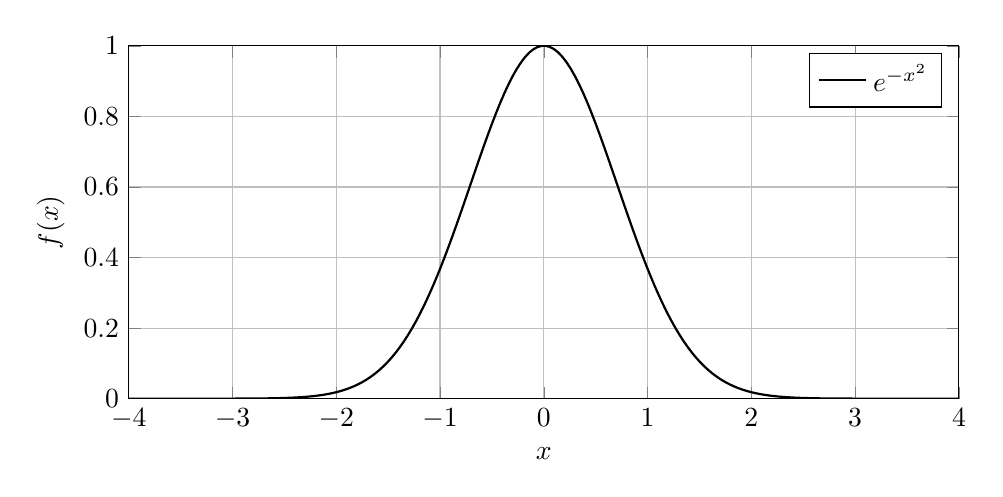
\begin{tikzpicture}
		\begin{axis}[
				xmin=-4, xmax=4,
				ymin=0,ymax=1,
				restrict y to domain = 0:3, domain=-4:4, width=\textwidth, height=0.5\textwidth, grid=major, samples=200,  ylabel=$f(x)$, xlabel=$x$, legend entries={$ e^{-x^2} $}]
			\addplot[black, thick] {e^(-x^2)};
		\end{axis}
	\end{tikzpicture}
\end{center}
Per calcolare l'integrale seguente posso spezzarlo in due parti
\[
	\int_{-\infty}^{\infty} e^{-x^2} \; dx= \int_{-\infty}^{a} e^{-x^2} \; dx + \int_{a}^{\infty} e^{-x^2} \; dx
\]
in questo caso $ a $ deve essere necessariamente 0 in quanto in 0 la funzione \underline{non} è definita
\subsubsection*{Esempio 2}
\begin{center}
	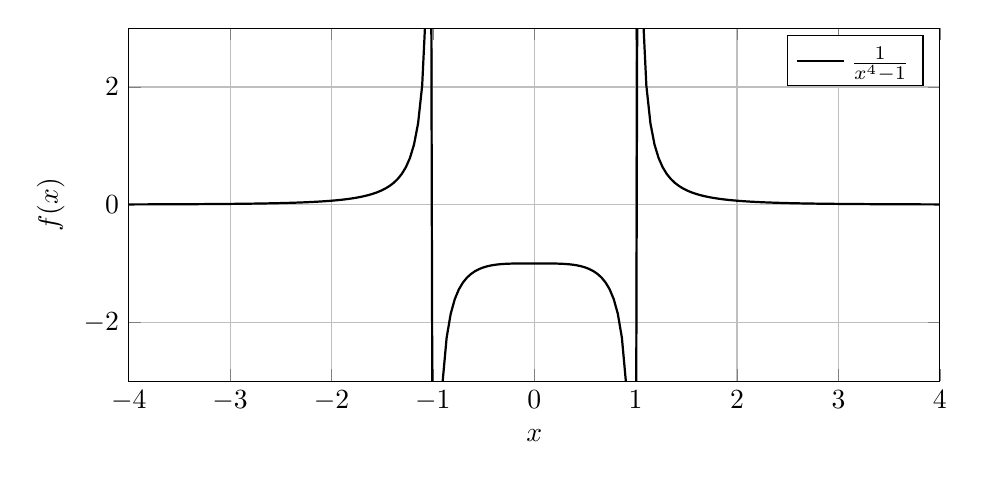
\begin{tikzpicture}
		\begin{axis}[
				xmin=-4, xmax=4,
				ymin=-3,ymax=3,
				restrict y to domain = -30:30, domain=-4:4, width=0.98\textwidth, height=0.5\textwidth, grid=major, samples=200,  ylabel=$f(x)$, xlabel=$x$, legend entries={$\frac{1}{x^{4}-1} $}]
			\addplot[black, thick] {1/(x^4-1)};
		\end{axis}
	\end{tikzpicture}
\end{center}
Per calcolare l'integrale
\[
	\int_{-\infty}^{\infty} \frac{1}{x^{4}-1} \; dx
\]
devo spezzarlo nei punti $ \left( -\infty, -3 \right) , \left( -3, -1 \right) , \left( -1, 0 \right) , \left( 0,1 \right) , \left( 1,3 \right) , \left( 3, +\infty \right)  $:
\[
	\int_{-\infty}^{\infty} \frac{1}{x^{4}-1} \; dx = \int_{-\infty}^{-3}  \; dx + \int_{-3}^{1}  \; dx + \int_{-1}^{0}  \; dx + \int_{0}^{1}  \; dx + \int_{1}^{3}  \; dx + \int_{3 }^{+\infty}  \; dx
\]
\subsubsection*{Esempio 3}
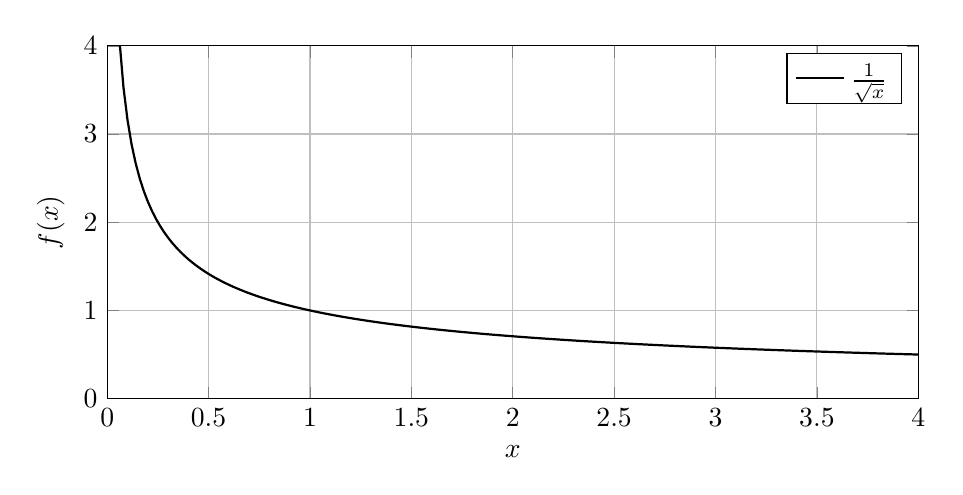
\begin{tikzpicture}
	\begin{axis}[
			xmin=0, xmax=4,
			ymin=0,ymax=4,
			restrict y to domain = 0:30, domain=0:4, width=0.98\textwidth, height=0.5\textwidth, grid=major, samples=200,  ylabel=$f(x)$, xlabel=$x$, legend entries={$ \frac{1}{\sqrt{x} }$}]
		\addplot[black, thick] {1/(sqrt(x))};
	\end{axis}
\end{tikzpicture}
\[
	\int_{0}^{5} \frac{1}{\sqrt{x} } \; dx= \lim_{a \to 0} \int_{a}^{5} \frac{1}{\sqrt{x} } \; dx
\]
\subsubsection*{Esempio 4}
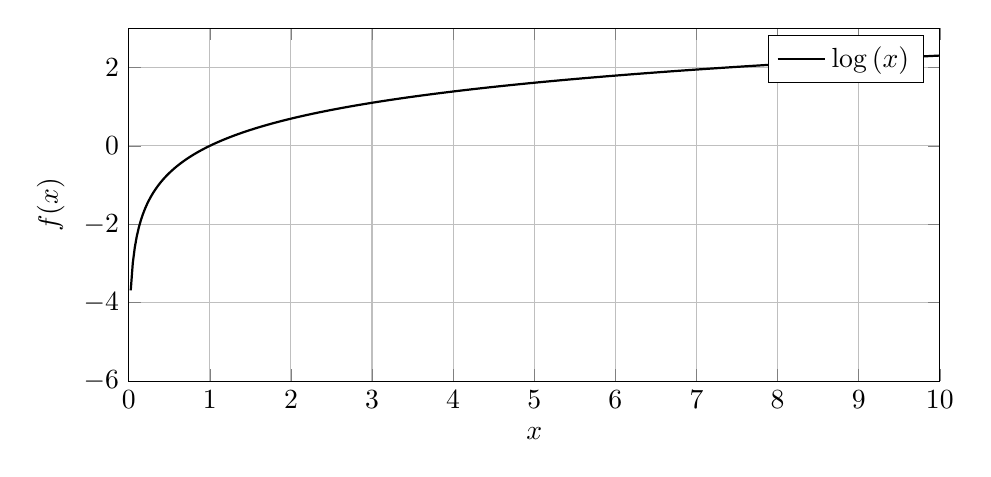
\begin{tikzpicture}
	\begin{axis}[
			xmin=0, xmax=10,
			ymin=-6,ymax=3,
			restrict y to domain = -400:30, domain=0:10, width=0.98\textwidth, height=0.5\textwidth, grid=major, samples=400,  ylabel=$f(x)$, xlabel=$x$, legend entries={$ \log \left( x \right) $}]
		\addplot[black, thick] {ln(x)};
	\end{axis}
\end{tikzpicture}
\[
	\int_{0}^{5} \log \left( x \right)  \; dx = \lim_{a \to 0} \int_{a}^{5} \log \left( x \right)  \; dx
\]
NB: un integrale improprio, essendo per definizione un limite, può non esistere. Ad esempio $ \int_{0}^{+\infty} \sin \left( x \right)  \; dx $ \underline{non esiste} in quanto oscilla infinitamente
\subsection{Teorema del confronto}
Spesso, vogliamo determinare se un integrale improprio corverga o meno, ma non sappiamo calcolarne una primitiva. In questi casi torna utile il \underline{teorema del comfronto}. L'idea è la seguente
\begin{itemize}
	\item Determino se funzioni campione delle quali so calcolare la primitiva convergono o meno
	\item Utilizzo queste funzioni, confrontandole con quella di cui devo determinare la convergenza
\end{itemize}
In particolare, le funzione "campione" che useremo saranno funzioni del tipo
\[
	\frac{1}{x^{\alpha }}
\]
in particolare queste funzioni vengono dette gli \underline{infiniti campione}.
\[
	\int_{1}^{+\infty} \frac{1}{x^{\alpha }} \; dx
\]
\begin{itemize}
	\item Converge se $ \alpha  >1 $
	\item Diverge se $ \alpha \le 1 $
\end{itemize}
Se invece considero l'integrale sull'intervallo $ \left( 0,1 \right)  $ ho che:
\[
	\int_{0}^{1} \frac{1}{x^{\alpha }} \; dx
\]
\begin{itemize}
	\item Converge se $ \alpha < 1 $
	\item Diverge se $ \alpha  \ge 1 $
\end{itemize}
Ciò risulta chiaro se osserviami i grafici delle funzioni
\begin{center}
	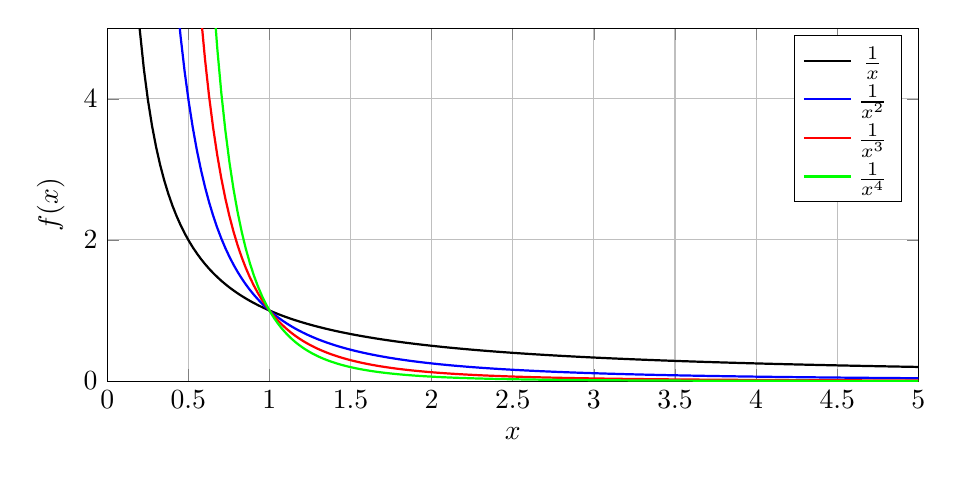
\begin{tikzpicture}
		\begin{axis}[
				xmin=0, xmax=5,
				ymin=0,ymax=5,
				restrict y to domain = 0:500, domain=0:5, width=0.98\textwidth, height=0.5\textwidth, grid=major, samples=200,  ylabel=$f(x)$, xlabel=$x$, legend entries={$\frac{1}{x}$,$\frac{1}{x^{2}}$, $\frac{1}{x^3}$ , $\frac{1}{x^4}$}]
			\addplot[black, thick] {1/x};
			\addplot[blue, thick] {1/x^2};
			\addplot[red, thick] {1/x^3};
			\addplot[green, thick] {1/x^4};
		\end{axis}
	\end{tikzpicture}
\end{center}
\begin{teorema}{Criterio del confronto}
	Sia $ f\left( x \right)  $ una funzione integranda, della quale voglio determinare l'ipotetica convergenza, su intervallo limitato o non. Sia $ g\left( x \right)  $ un infinito campione del tipo $ \frac{1}{x^{\alpha }} $. Se $ 0 \le f\left( x \right) \le g\left( x \right)  $ almeno in un intorno del problema (estremi intervallo integrazione, $ +\infty, - \infty $), allora:
	\[
		\text{ se }\int_{E} g\left( x \right)  \; dx \text{ converge } \Rightarrow \int_{E} f\left( x \right) \; dx \text{ converge }
	\]
	\[
		\text{ se }\int_{E} f\left( x \right)  \; dx \text{ diverge } \Rightarrow \int_{E} g\left( x \right) \; dx \text{ diverge }
	\]

\end{teorema}

\begin{teorema}{Teorema del confronto asintotico}
	Supponiamo che $ f\left( x \right) \ge 0 $ e $ g\left( x \right) > 0 $. Allora se
	\[
		\lim_{x \to x_0} \frac{f\left( x \right) }{g\left( x \right) } \neq 0, \infty
	\]
	allora l'integrale delle due funzioni si comporta nello stesso modo (convergenza/divergenza è uguale)

\end{teorema}

Se $ \lim_{x \to x_0} \frac{f\left( x \right) }{g\left( x \right) }  = 0 $
\begin{itemize}
	\item Se $ \int_{E} g\left( x \right)  \; dx $ converge allora $ \int_E f\left( x \right)  \; dx $ converge
	\item Altrimenti non so dire nulla
\end{itemize}
Se $ \lim_{x \to x_0} \frac{f\left( x \right) }{g\left( x \right) }  = +\infty $
\begin{itemize}
	\item Se $ \int_{E} g\left( x \right)  \; dx $ diverge allora $ \int_E f\left( x \right)  \; dx $ diverge
	\item Altrimenti non so dire nulla
\end{itemize}
\subsubsection*{Assoluta integrabilità}
Questo teorema può essere utile per applicare il teorema del confronto su funzioni che non sono sempre $ \ge 0  $ o $ \le 0 $.

\begin{teorema}{Assoluta integrabilità}
	\[
		\text{ Se }\int_{E}\left|f\left( x \right) \right| \; dx \text{ converge } \Rightarrow \int_{E} f\left( x \right)  \; dx \text{ converge }
	\]
	\[
		\text{ Se } \int_{E}\left|f\left( x \right) \right| \; dx \text{ diverge } \rightarrow \text{ non posso affermare nulla }
	\]

\end{teorema}
Ad esempio:
\[
	\int_{0}^{+ \infty} \frac{\sin \left( x^2 \right) }{x^3} \; dx
\]
non posso utilizzare il teorema del confronto asistotico perchè il seno non è sempre positivo. Posso tuttavia analizzare la funzione
\[
	\int_{0}^{+ \infty} \frac{\left|\sin \left( x^2 \right) \right| }{x^3} \; dx
\]
\begin{itemize}
	\item Considero che la funzione integranda è maggiorata dalla funzione $ \frac{2}{x^3} $
	      \[
		      \frac{\left|\sin \left( x^2 \right) \right|}{x^3} \le \frac{2}{x^3}
	      \]
	\item Siccome la funzione $ \frac{2}{x^3} $ converge, allora anche $ \frac{\left|\sin \left( x^2 \right) \right|}{x^3} $ converge.
	\item  Se $ \frac{\left|\sin \left( x^2 \right) \right|}{x^3} $ converge, per il teorema della assoluta integrabilità, anche $\frac{\sin \left( x^2 \right) }{x^3} $
\end{itemize}
\subsection{Trucco dell'integrazione per parti}
Se devo decretare la convergenza/divergenza di un integrale improprio posso utilizzare il metodo dell'integrazione per parti. Consideriamo il seguente esempio:
\subsubsection*{Esempio 1}
\[
	\int_{1}^{ + \infty} \frac{\sin x}{x} \; dx
\]
non posso applicare il teorema del confronto in quanto ogni funzione $ \frac{1}{x^{\alpha }} $ con $ \alpha \ge 1 $  è definitivamente minore di $ \frac{\sin x}{x} $ e converge. Contrariamente, $ \frac{1}{x} $ è definitivamente maggiore, però diverge per $ x \to \infty $	e non posso dunque affermare nulla. Se integro per parti tuttavia:
\[
	\int \frac{\sin x}{x} \; dx = \frac{1}{x} \left( - \cos  x \right) - \int -\frac{1}{x^2}\left( -\cos x \right)
\]
applicando il limite posso decretare che l'integrale converge
\subsubsection*{Esempio 2}
\[
	\int_{0}^{+\infty} \cos \left( x^2 \right)  \; dx
\]
stranamente, questo integrale converge ad un numero reale. Non posso applicare assoluta integrabilità perchè, chiaramente, l'integrale del suo valore assoluto diverge. Provo moltiplicando e dividendo per $ x $ (in modo da ottenere la derivata della composta), per poi integrare per parti:
\[
	\int \cos \left( x^2 \right) = \int \frac{1}{x} x \cos \left( x^2 \right) = \left( -\frac{1}{x^2} \right)  \left( \frac{1}{2}\sin \left( x^2 \right) \right)  - \int  \left( -\frac{1}{x^2} \right) \frac{1}{2}\sin \left( x^2 \right)
\]
Visto che ogni membro converge, posso affermare che $ \int_{0}^{+ \infty} \cos \left( x^2 \right)  \; dx $ \underline{converge}

\section{Equazioni differenziali}
\subsection{Definizioni}
\begin{definizione}{Equazione differenziale}
	Con il termine \underline{equazione differenziale} si intende una relazione tra una \underline{funzione incognita} e le sue derivate. Posso interpretarla come una funzione di più variabili:
	\[
		F\left( t, u\left( t \right) , u'\left( t \right) ,\ldots, u^{\left( k \right) }\left( t \right)  \right)=0
	\]
	dove $ t, u\left( t \right) ,\ldots, u^{\left( k \right) }\left( t \right)  $ sono le incognite dell'equazione differenziale

\end{definizione}
La soluzione di un'equazione differenziale è un'equazione che risolve l'uguaglianza specificata
\begin{itemize}
	\item \textbf{Ordine}: l'ordine di un'equazione differenziale è uguale al massimo ordine di derivazione presente nell'equazione
	\item \textbf{Eq diff. in forma normale}: una eq. diff. si dice in forma normale se si può "isolare" la derivata di ordine massimo:
	      \[
		      u^{\left( k \right) } = \Phi \left( u^{\left( k-1 \right) },\ldots, u\left( t \right) ,t \right)
	      \]
	\item \textbf{Eq. diff. autonoma}: se la incognita $ t $ compare solo come incognita della funzione incognita (e non compe coefficiente):
	      \[
		      u^{\left( k \right) }+ u ^{\left( k-1 \right) }+\ldots+u' + u =0
	      \]
	\item \textbf{Eq. diff. a variabili separabili}: se è del \underline{primo ordine}, scritta in \underline{forma normale} e si può scrivere nella seguente forma:
	      \[
		      u'= f\left( t \right) g\left( u \right)
	      \]
	\item \textbf{Eq. diff. lineare}: se la funzione $ u $ e le sue derivate non sono presenti all'interno di funzioni. Ha forma del tipo:
	      \[
		      a_k\left( t \right) u^{\left( k \right) }+ a_{k-1}\left( t \right) u^{\left( k-1 \right) }+\ldots+ a_1\left( t \right) u'+ a_0\left( t \right) u = f\left( t \right)
	      \]
	      \begin{itemize}
		      \item $ a_0\left( t \right) , a_1\left( t \right) ,\ldots, a_k\left( t \right)  $ sono detti \underline{coefficienti}
		      \item $ f\left( t \right)  $ è detto \underline{termine noto}
		      \item Se $ f\left( t \right) =0 $ l'equazione lineare si dice \underline{omogenea}
		      \item Se $ a_0\left( t \right) , a_1\left( t \right) ,\ldots, a_k\left( t \right)  $ sono costanti l'equazione è detta a \underline{coefficienti costanti}
	      \end{itemize}
\end{itemize}

\subsubsection*{Esempio 1}
\[
	f'\left( x \right) = f\left( x \right)
\]
Quale equazione ha la derivata uguale alla equazione stessa? Esattamente l'esponenziale. Più precisamente le soluzioni di questa equazione sono \underline{infinite} ed identificate dalla seguente funzione:
\[
	k e^{x}
\]
\subsubsection*{Esempio 2}
\[
	f'\left( x \right) = - f\left( x \right) ^2
\]
una qualsiasi soluzione del seguente tipo risolve la seguente eguaglianza:
\[
	f\left( x \right) = \frac{1}{t + c}
\]
\subsubsection*{Esempio 3}
\[
	f''\left( x \right) = - f\left( x \right)
\]
noto che una soluzione è $ n\left( x \right) = \cos \left( x \right)  $. La famiglia delle soluzioni è $ n\left( x \right) = c \cos \left( t \right)  , c \in  \R$. Ancora più in generale, ogni funzione del tipo:
\[
	f\left( x \right) = c_1 \cos t\left( x \right)  + c_2 \cos \left( x \right)
\]
soddisfa l'eguaglianza. Nota che il numero di parametri che ottengo dipende dall'\underline{ordine} dell'equazione
\subsection{Problemi di Cauchy}
Negli esempi precedenti ho ottenuto le cosiddette \underline{soluzioni generali} delle equazioni differenziali. Se impongo un'ulteriore condizione sulla condizione generale ottengo il valore della costante (o delle costanti) in corrispondenza del quale è risolto il problema di Cauchy.
\subsubsection*{Esempio 1}
\[
	\begin{cases}
		u'\left( t \right) = u\left( t \right) \\
		u\left( 0 \right) = 5
	\end{cases}
\]
\begin{itemize}
	\item Condizione dell'equazione differenziale: $ ce^{t} $
	\item Condizione iniziale: $ u\left( 0 \right) = ce^{0} \rightarrow c = 5 $
\end{itemize}
Quindi la soluzione è $ 5 e ^{t} $
\subsubsection*{Esempio 2}
\[
	\begin{cases}
		u' = - u^2 \\
		u\left( 5 \right) = 7
	\end{cases}
\]
\begin{itemize}
	\item Soluzione dell'equazione differenziale: $ \frac{1}{t + c} $
	\item Condizione iniziale: $ u\left( 5 \right) = 7 $
\end{itemize}
\hr
Nota che le condizioni delle equazioni differenziali ordinarie devono essere tante quanto è l'ordine dell'equazione differenziale: ottengo infatti un sistema in cui devo trovare il valore a tutte le costanti ottenute trovando la \underline{soluzione generale}
\subsubsection*{Esempio 3}
\[
	\begin{cases}
		u'' + 3 u' = u^2 + t^2 \\
		u \left( 5 \right) = 7 \\
		u' \left( 5 \right) = 22
	\end{cases}
\]
è un problema di Cauchy.
\[
	\begin{cases}
		u'' + 3 u' = u^2 + t^2 \\
		u \left( 5 \right) = 7 \\
		u' \left( 6 \right) = 22
	\end{cases}
	\quad
	\begin{cases}
		u'' + 3 u' = u^2 + t^2 \\
		u \left( 5 \right) = 7 \\
		u'' \left( 5 \right) = 22
	\end{cases}
\]
non sono problemi di Cauchy. Più in generale
\begin{definizione}{Problema di Cauchy}
	Data un'equazione differenziale ordinaria di ornine $ n $, un problema di Cauchy associato deve:
	\begin{itemize}
		\item Specificare le \underline{condizioni iniziali} in uno stesso punto
		\item Specificare le condizioni iniziali per le derivate di ordine $ 0,1,\ldots, n-1 $
	\end{itemize}
\end{definizione}

\begin{teorema}{Teorema di esistenza}
	Consideriamo il problema di Cauchy per una equazione differenziale ordinaria. Defininiamo la funzione:
	\[
		u^{\left( k \right) }= \Phi \left( u, u',u'',\ldots,u^{\left( k-1 \right) },t \right)
	\]
	Se $ \Phi   $ è continua in ogni variabile allora esiste sempre \underline{almeno una soluzione}

\end{teorema}

la funzione $ \Phi $ è una funzione a più variabili. La sua continuità o la sua derivabilità si decreta "congelando" tutte le variabili meno che una e studiandone continuità/derivabilità
\begin{teorema}{Teorema di unicità}
	Consideriamo il problema di Cauchy per una equazione differenziale ordinaria. Defininiamo la funzione:
	\[
		u^{\left( k \right) }= \Phi \left( u, u',u'',\ldots,u^{\left( k-1 \right) },t \right)
	\]
	Se $ \Phi  $ è \underline{derivabile} in tutte le variabili, allora la soluzione è \underline{unica}

\end{teorema}
il cosiddetto "pennello" di Peano è un problema di Cauchy che presenta infinite soluzioni:
\[
	\begin{cases}
		u'= 3 \left|u\right|^{\frac{2}{3}} \\
		u\left( 0 \right) =0
	\end{cases}
\]
La funzione $ 3 \left|u\right|^{\frac{2}{3}} $ non è derivabile, quindi la soluzione \underline{non} è unica. Nota che sia $ u=0 $ che $ u=t^3 $ sono soluzioni del problema. Il problema presenta più di una soluzione
\subsection{Edo a variabili separabili}
\[
	u' = f\left( t \right) g\left( u \right)
\]
Per trovare la soluzione ci sono 3 passaggi:
\begin{itemize}
	\item Separazione
	\item Integrazione
	\item Ricavare
\end{itemize}
Esempio:
\[
	u' = t^3 u^2
\]
\begin{itemize}
	\item \underline{Separo} le variabili: metto tutto ciò che dipende da $ u $ a sinistra e tutto ciò che dipende da $ t $ a destra, usando questo trucchetto bovino:
	      \[
		      \frac{du}{dt}= t^3 u^2 \rightarrow \frac{du}{u^2}= t_3 dt
	      \]
	\item \underline{Integro} da entrambe le parti:
	      \[
		      \int \frac{du}{u^2}= \int t_3 dt \rightarrow - \frac{1}{u}= \frac{1}{4} t^{4} + c
	      \]
	\item \underline{Ricavo} $ u $ in funzione di $ t $:
	      \[
		      u\left( t \right) = \frac{- 4}{t ^{4} + c} \quad c \in  \R
	      \]
\end{itemize}
\hr

Se all'edo è associato un problema di Cauchy è necessario studiare la soluzione: il dominio della soluzione varia in base al valore di $ c $ trovato. Per questa ragione devo restringere il dominio della funzione trovata.
\textbox{Devo restringere il dominio della funzione trovata al massimo insieme di definizione che contiene il punto indicato nella condizione iniziale}
\subsection{Tempo di vita ed esempi}
\begin{definizione}{Tempo di vita}
	Trovata la funzione $ u\left( t \right)  $ soluzione di un problema di Cauchy, si dice tempo di vita l'\underline{estremo superiore} dell massimo insieme di definizione contenente il punto $ t_0 $ che esprime la condizione di essistenza.
	\begin{itemize}
		\item Se $ T=+ \infty $ si dice che $ f\left( t \right)  $ ha \underline{esistenza globale} nel futuro
		\item Se $ T < +\infty $ ci sono due casi:
		      \begin{itemize}
			      \item Se $ \lim_{x \to T^{-}} f\left( t \right) = \pm \infty  \rightarrow$ \underline{blow up}
			      \item Se non c'è blow up ma $ u\left( t \right)  $ esce dal dominio di una o più funzioni presenti nell'equazione differenziale $ \rightarrow $ \underline{break down}. In genere (ma non sempre) questo si dtraduce nella seguente condizione
			            \[
				            \lim_{x \to T^{-}} f'\left( t \right) = \pm \infty
			            \]
		      \end{itemize}
	\end{itemize}

\end{definizione}

\subsubsection*{Esempio Cauchy 1}
\[
	\begin{cases}
		u' = t^3 u^2 \\
		u\left( 0 \right) = -5
	\end{cases}
\]
L'edo ha soluzione
\[
	u\left( t \right) = \frac{-4}{t ^{4}+ c}
\]
\begin{itemize}
	\item Determino $ c $ :
	      \[
		      u\left( 0 \right) = -\frac{4}{c} \rightarrow c = \frac{4}{5}
	      \]
	      quindi il problema di Cauchy ha soluzione $ u\left( t \right)= -\frac{4}{t ^{4}+ \frac{4}{5}} $
	\item Il massimo dominio di definizione contentente $ 0 $ è $ \R $, quindi $ u\left( t \right)  $ ha \underline{esistenza globale} sia nel passato che nel futuro
\end{itemize}
\subsubsection*{Esempio Cauchy 2}
\[
	\begin{cases}
		u' = t^3 u^2 \\
		u\left( 0 \right) = 0
	\end{cases}
\]
L'edo ha soluzione
\[
	u\left( t \right) = \frac{-4}{t ^{4}+ c}
\]
\begin{itemize}
	\item Determino $ c $ :
	      \[
		      u\left( 0 \right) = -\frac{4}{c} =0
	      \]
	      Cosa faccio? Non posso risolvere l'equazione ottenuta.
\end{itemize}
In questo caso il problema di Cauchy \underline{ha una soluzione}. Tale soluzione si ottiene risolvendo la condizione iniziale:
\[
	u\left( t \right) =0
\]
in questo modo soddisfo sia la condizione iniziale $ u\left( 0 \right) =0 $ e l'equazione differenziale in quanto $ u' = t^3 u^2 $
\subsubsection*{Esempio Cauchy 3}
\[
	\begin{cases}
		u' = u^3 t^2 \\
		u\left( 0 \right) =5
	\end{cases}
\]

La soluzione dell'equazione differenzile è:
\[
	u\left( t \right) = \pm \sqrt{\frac{3}{c-2t^3}}
\]
Devo sceglere la radice positiva in quanto la condizione iniziale impone $ u\left( 0 \right) =5 $.Impongo la condizione iniziale e ottengo
\[
	\sqrt{\frac{3}{c}} \rightarrow c = \frac{3}{25}
\]
Quindi il problema di Cauchy ha soluzione
\[
	u\left( t \right) = \sqrt{\frac{3}{\frac{3}{25} - 2 t ^3}} = \sqrt{ \frac{75}{3 - 50 t^3}}
\]
Posso procedere ora studiando la soluzione:
\[
	3 - 50 t^3 > 0 \rightarrow t < \sqrt[3]{\frac{3}{50}}
\]
La funzione è quindi definita su $ \left( - \infty, \sqrt[3]{\frac{3}{50}}  \right)  $. Posso dunque affermare che il \underline{tempo di vita} della funzione è $ T= \sqrt[3]{\frac{3}{50}} $. Visto che $ \lim_{t \to \sqrt[3]{\frac{3}{50}}^{-}} u\left( t \right)   = + \infty $ la funzione ha un \underline{blow up}
\subsubsection*{Esempio Cauchy 4 parametrico}
\[
	\begin{cases}
		u' = u^3 t^2 \\
		u\left( 0 \right) = \alpha
	\end{cases}
\]
Per quali valori di $ \alpha  $ ho esistenza globale nel futuro?
\vskip3mm
Eseguo tutti i passi fatti per trovare le soluzioni del problema di Cauchy rispetto al parametro $ \alpha  $ e ottengo:
\[
	u\left( t \right) = \pm \sqrt{\frac{3}{-2t^3 + \frac{3}{\alpha ^2}}}
\]
\subsubsection*{Esempio Cauchy 4}
\[
	\begin{cases}
		u'= u \sin \left( t \right) \\
		u\left( 0 \right) = -2
	\end{cases}
\]
\begin{itemize}
	\item Separo:
	      \[
		      \frac{du}{u}= \sin \left( t \right) dt
	      \]
	\item Integro:
	      \[
		      \int \frac{du}{u}= \int \sin \left( t \right) dt \rightarrow \log \left| u\right|= - \cos t\left( t \right)  + c
	      \]
	\item Ricavo (tolgo il valore assoluto introducento $ \pm $):
	      \[
		      u\left( t \right) = \pm e^{-\cos \left( t \right)  + c}= c e ^{-\cos \left( t \right) }
	      \]
	\item Determino $ c $
	      \[
		      u\left( 0 \right) = -2 \rightarrow c = -2e
	      \]
\end{itemize}
La soluzione al problema di Cauchy è quindi:
\[
	u\left( t \right) = -2e \cdot e^{-\cos \left( t \right) }
\]
\subsubsection*{Esempio 6 Cauchy}
\[
	\begin{cases}
		u' = -\frac{1}{u} \\
		u\left( 0 \right) =4
	\end{cases}
\]
\begin{itemize}
	\item Separo:
	      \[
		      \frac{du}{dt}= -\frac{1}{u} \rightarrow u du = -dt
	      \]
	\item Integro e ricavo:
	      \[
		      u\left( t \right) = \pm \sqrt{c - 2t}
	      \]
	\item Determino $ c $
	      \[
		      u\left( 0 \right) = \pm \sqrt{c} =4 \rightarrow c=14 c=14
	      \]
\end{itemize}
La soluzione al problema di Cauchy è quindi:
\[
	u\left( t \right) = \sqrt{16-2t}
\]
Studio la soluzione
\begin{itemize}
	\item La soluzione è definita se $ 16 - 2t \ge 0  \rightarrow t \le 8$
	\item L'intervallo massimale di esistenza del problema di Cauchy è $ \left( -\infty, 8 \right)  $
	\item Il tempo di vita è $ T=8 $
	\item Visto che $ \lim_{t \to T^{-}} u\left( t \right)  = 0 $, \underline{non} c'è blow-up, ma c'è break-down, infatti $ -\frac{1}{u}=-\frac{1}{\sqrt{16-2t} } $ ha dominio $ (-\infty, 8] $, mentre la funzione soluzione, ossia $ \sqrt{16-2t}  $ ha dominio $ \left( -\infty, 8 \right)  $, ossia \underline{esce} da dominio di definizione. Posso anche verificare con la derivata in questo caso:
	      \[
		      \lim_{t \to 8^{-}} u\left( t \right)  = - \infty
	      \]
\end{itemize}


\subsection{Equazioni differenziali lineari}
\textbox{Fatto generale importante: se tutti i coefficienti dell'equazione sono funzioni continuo in un intervallo $ \left( a,b \right)  $, allora esiste una soluzione almeno nell'intervallo $ \left( a,b \right)  $}
\teorema{Spazio soluzioni equazione differenziale lineare}{
	L'insieme di tutte le soluzione di una equazione differenziale lineare di ordine $ n $ \underline{omogenea} ( $ f\left( t \right) =0 $) è uno spazio vettoriale di ordine $ n $. La soluzione dell'equzione si può dunque esprimere come combinazione lineare fra gli elementi di una sua \underline{qualsiasi} base
}
Stringi stringe questo equivale a dire che mi ritrovero tante costanti $ c_0,c_1,\ldots, c_{k-1}, c_{k} $ quante l'ordine della suddetta equazione
\teorema{Soluzione equazioni differenziali non omogenee}{
	Una equazione differenziale lineare \underline{non omogenea} ha una soluzione che si può scrivere nella seguente forma:
	\[
		u\left( t \right) = c_1 u_1\left( t \right) + c_2u_2\left( t \right) + \ldots + c_nu_n\left( t \right) + \overline{u}\left( t \right)
	\]
	dove
	\begin{itemize}
		\item $ u_1\left( t \right) ,\ldots, u_n\left( t \right)  $ solo gli elementi di una base qualsiasi dell'insieme soluzione dell'equazione \underline{omogenea} associata (ottenuta mettengo $ f\left( t \right)=0  $)
		\item $ \overline{u}\left( t \right)  $ è una soluzione \underline{qualsiasi} del sistema \underline{non omogeneo}
	\end{itemize}
}
La funzione $ \overline{u}\left( t \right)  $ può essere trovata adoperando alcuni stratagemmi. In reltà però non abbiamo un metodo che ci garantisca di trovarla. Dobbiamo tendenzialmente procedere "a tentoni"

\section{Tecniche risolutive equazioni differenziali}
\subsection{Edo lineari di primo ordine}
\subsubsection*{Equazioni a variabili separabili}
\label{edol1}
La risoluzione di equazioni lineari a coefficienti costanti omogenee è immediata e si vede ad occhio:
\[
	au' + bu = 0 \rightarrow u' = -\frac{b}{a}u
\]
l'esponenziale fornisce una soluzione a questa equazione, in particolare
\[
	ce ^{-\frac{b}{a}t}
\]
è la famiglia di soluzioni dell'equazione differenziale

\subsubsection*{Equazioni lineari non omogenee di primo ordine}
Per risolvere un'equazione lineare non necessariamente autonoma del primo ordine con la seguente forma
\[
	u'\left( t \right) + a\left( t \right) u\left( t \right) = b\left( t \right)
\]
posso utilizzare la tecnica del fattore integrante
\begin{itemize}
	\item Trovo una primitiva qualsiasi si $ a\left( t \right)  $
	      \[
		      A'\left( t \right)=a\left( t \right)
	      \]
	\item Moltiplico entrambi i membri dell'equazione per $ e^{A\left( t \right) } $
	\item Ottengo la derivata di un \underline{prodotto di funzioni} a sinistra
	      \[
		      u'\left( t \right)e^{A\left( t \right) } + a\left( t \right) u\left( t \right) e^{A\left( t \right) } = b\left( t \right) e^{A\left( t \right) }
	      \]
	      \[
		      d \left[ ue^{A\left( t \right) } \right] = b\left( t \right) e^{A\left( t \right) }
	      \]
	\item Integro da entrambe le parti e ricavo $ u\left( t \right)  $
\end{itemize}


\subsection{Edo lineari di secondo ordine}
\label{edol2}
\begin{itemize}
	\item Scrivo polinomio associato a equazione lineare
	\item Trovo zeri del polinomio associato
	\item Seguo le soluzioni in base ai seguenti casi in base delta del polinomio
\end{itemize}
In particolare, avrò 3 casi a seconda del $ \Delta  $ del polinomio
\begin{itemize}
	\item $ \Delta  > 0 $
	      \begin{itemize}
		      \item Ho due radici reali distinte: $ \lambda , \mu \quad \lambda \neq \mu  $
		      \item La base dell'insieme soluzione è costituita da
		            \[
			            e^{\lambda t} , \quad e^{\mu t}
		            \]
		      \item La funzione soluzione è quindi costituita da:
		            \[
			            c_1e^{\lambda t} + c_2e^{\mu t}
		            \]
	      \end{itemize}
	\item $ \Delta =0 $
	      \begin{itemize}
		      \item Ho una radice con molteplicità doppia $ \lambda  $
		      \item La base dell'insieme soluzione è costituita da:
		            \[
			            e^{\lambda  t}, \quad te^{\lambda t}
		            \]
		      \item La funzione soluzione è quindi costituita da:
		            \[
			            c_1e^{\lambda t} + c_2te^{\lambda  t}
		            \]
	      \end{itemize}
	\item $ \Delta <0 $
	      \begin{itemize}
		      \item Il polinomio ha due radici complesse coniugate di forma $ \alpha  \pm i \beta \quad \alpha ,\beta  \in  \R $
		      \item La base dell'insieme soluzione è costituita da:
		            \[
			            e^{\alpha t}\cos \left( \beta  t \right) , \quad  e ^{\alpha t}\sin \left( \beta t \right)
		            \]
		      \item La funzione soluzione è quindi costituita da:
		            \[
			            c_1 e^{\alpha t}\cos \left( \beta  t \right)  +c_2 e ^{\alpha t}\sin \left( \beta t \right)
		            \]
	      \end{itemize}
\end{itemize}
\subsection*{Esempi equazioni lineari}

\subsubsection*{Esempio 1}
\[
	u'' + 3u' -4u =0
\]
ha polinomio associato
\[
	x^2 + 3x - 4 \rightarrow \left( x+4 \right) \left( x-1 \right)
\]
quindi ho base
\[
	e^{-4t}, e^{t}
\]
\subsubsection*{Esempio 2}
\[
	u'' - 6u + 9u =0 \rightarrow x^2 - 6x + 9 =0 \rightarrow \left( x-3 \right) ^2 =0
\]
che ha quindi base
\[
	e^{3t}, t e ^{3t}
\]
\subsubsection*{Esempio 3}
\[
	u'' + 8u + 17 u =0 \rightarrow x^2 + 8x + 17 =0
\]
trova radici
\[
	x_{1 /2} -4 \pm \sqrt{16-17} = -4 \pm i
\]
quindi ho radici complesse con $ \alpha  = -4 $ e $ \beta  = 1 $. La base sarà:
\[
	e ^{ -4t}\cos \left( t \right) , e ^{ -4t}\sin \left( t \right)
\]
\subsubsection*{Esempio 4}
\[
	u'' - 4u' =0 \rightarrow x^2 - 4x =0 \rightarrow x\left( x-4 \right)
\]
Quindi ho base associata
\[
	e^{0t}=1, e ^{4t}
\]
\subsubsection*{Esempio 5}
\[
	u'' - 4u =0 \rightarrow x^2 - 4	=0 \rightarrow \left( x-2 \right) \left( x+2 \right) =0
\]
Quindi ho base associata
\[
	e^{2t}, e^{-2t}
\]
NB: se la base è del tipo $ e^{\alpha t}, e^{-\alpha t}$, allora un'altra base può essere ottenuta dividendo i componenti della base per 2:
\[
	\frac{e^{2t}+e^{-2t}}{2}=\cosh \left( 2t \right)  , \quad \frac{e^{2t}-e^{-2t}}{2} = \sinh \left( 2t \right)
\]
\subsubsection*{Esempio 6}
\[
	u'' + 4 u =0	\rightarrow x^2 + 4 =0
\]
il polinomio associato ha due radici complesse coniugate $ x_{1 / 2} = \pm 2i$. Quindi $ \alpha  =0 $ e $ \beta  = 2 $ e la base sarà
\[
	e ^{ 0t}\cos \left( 2t \right) = \cos \left( 2t \right) , e^{0t}\sin \left( 2t \right) =\sin \left( 2t \right)
\]
\subsection{Equazioni lineari omogenee di ordine m}
Generalizzando quanto detto nella \textit{sezione \ref{edol1}} e \textit{\ref{edol2}} posso ragionare cercando gli elementi della base della famiglia delle soluzioni seguendo le seguenti regole.
\textbox{Innanzitutto, per il teorema fondamentale dell'algebra, un polinomio di grado $ n $ ha sempre $ n $ radici \underline{complesse}}
\begin{itemize}
	\item Una radice reale $ \lambda  $ di molteplicità 1 produce un elemento di forma
	      \[
		      e^{\lambda t}
	      \]
	\item Una radice reale $ \lambda  $ di molteplicità $ m $ produce $ m $ elementi della seguente forma:
	      \[
		      e^{\lambda t}, te^{\lambda t}, t^2 e ^{\lambda t},\ldots, t ^{m-1}e^{\lambda t}
	      \]
	\item Una coppia di radici complesse coniugate di forma $  \alpha  \pm i \beta  $ con molteplicità 1 produce 2 elemendi di base:
	      \[
		      e^{\alpha t} \cos \left( \beta  \right) , \quad  e ^{\alpha t}\sin \left( \beta t \right)
	      \]
	\item Una coppia di radici complesse coniugare di forma $ \alpha  \pm i \beta  $ con molteplicità $ m $ produce $ 2m $ elementi di base con forma:
	      \[
		      e^{\alpha t} \cos \left( \beta  \right) ,  e ^{\alpha t}\sin \left( \beta t \right), te^{\alpha t} \cos \left( \beta  \right) ,  te ^{\alpha t}\sin \left( \beta t \right),\ldots,  t ^{m-1}e^{\alpha t} \cos \left( \beta  \right) ,  t^{m-1}e ^{\alpha t}\sin \left( \beta t \right)
	      \]
\end{itemize}
\subsection{Equazioni lineari non omogenee} \label{edononomogenee}
\subsubsection*{Tipo esponenziale}
\label{tipoesponensiale}
Per risolvere equazioni differenziali non omogenee del tipo
\[
	au''+ bu' + cu = e^{\lambda_1 t}
\]
bisogna procedere a tentoni, prendendo come funzione (che tipo di funzioni, tramite loro combinazioni lineari, possono darmi una funzione del tipo $ \lambda_0 e^{\lambda_1 t} $):
\[
	\overline{u}\left( t \right) = \lambda  e^{\lambda_1 t}
\]
\begin{itemize}
	\item Prendo funzione $ \overline{u}\left( t \right)  $ del tipo $ \lambda e^{\lambda_1 t} $
	\item Vedo se esiste un valore di $  \lambda  $ che soddisfi l'equazione
	\item Ho due casi:
	      \begin{itemize}
		      \item Se $ \overline{u} \left( t \right)  $ \underline{non} è soluzione dell'equazione omogenea associata (ossia $ au''+ bu' + cu = 0$). Allora posso trovare un valore di $ \lambda $ che risolva l'equazione
		      \item Se $ \overline{u}\left( t \right)  $ è soluzione dell'equazione omogenea associata allora è impossibile trovare un valore di $ \lambda  $ che soddisfi l'equazione. Devo provare con $ \overline{u}\left( t \right) = \lambda t e^{\lambda_1 t} $
		      \item Se non funziona nemmeno con questo devo provare con $ \overline{u}\left( t \right) = \lambda t^2e^{\lambda_1 t} $ e così via per ogni potenza di $ t $
	      \end{itemize}
\end{itemize}
\subsubsection*{Tipo trigonometrico}
Per risolvere equazioni differenziali non omogenee del tipo
\[
	au''+ bu' + cu = \sin \left( at \right) \quad au''+ bu' + cu = \cos \left( at \right)
\]
devo procedere a tentoni prendendo come funzione $ \overline{u} $
\[
	\overline{u}\left( t \right) = \lambda \cos \left( at \right) + \mu \sin \left( at \right)
\]
Alla fine otterrò una somma di seni e coseni sia a destra che a sinistra. Posso trovare i valori di $ \lambda  $ e $ \mu  $ risolvendo un sistema
\vskip3mm
NB: se la funzione $ \overline{u}\left( t \right)  $ è soluzione del sistema omogeneo associato, devo provare moltiplicando per le potenze di $ t $, come in \textit{sottosezione \ref{tipoesponensiale}}
\subsubsection*{Tipo polinomiale}
Per risolvere equazioni differenziali non omogenee del tipo
\[
	au''+ bu' + cu = p\left( t \right)
\]
devo procedere a tentoni prendendo come funzione $ \overline{u} $
\[
	\overline{u}\left( t \right) = k_1t ^{n}+ k_2 t ^{n-1}+\ldots+k_{n-1}t+ k_n
\]
ossia il polinomio generico completo di grado $ n $, dove $ n $ è il grado del polinomio $ p\left( t \right)  $
\vskip3mm
NB: questo tentativo non funziona quando $ 0 $ è tra le radici del polinomio dell'omogenea associata
\hr
\textbox{Se il termine noto dell'equazione differenziale è dato dalla somma di diversi tipi(esponenziale, trigonometrico, polinomiale) la soluzione sarà data dalla somma delle soluzioni. Es
}
Esempio:
\[
	u'' + 3u' - 4u = \cos \left( 2t \right) + t^3 + e^{5t}+ e^{-4}t
\]
risolvo le equazioni differenziali non omogenee:
\begin{align*}
	u'' + 3u' - 4u & =  \cos \left( 2t \right) \\
	u'' + 3u' - 4u & = t^3                     \\
	u'' + 3u' - 4u & =  e^{5t}                 \\
	u'' + 3u' - 4u & =  e^{-4t}
\end{align*}
la soluzione dell'equazione differenziale originaria è data dalla somma delle soluzioni trovate, per via della \underline{linearità}
\subsection{Metodo di variazione delle costanti}
Per risolvere equazioni diff. lineari \underline{non} omogenee posso utilizzare anche questo metodo oltre che il medoto "a tentoni" spiegato in \textit{sezione \ref{edononomogenee}}. Esempio:
\[
	u''-3u' + 2u =t
\]
\subsubsection*{Risoluzione tramite metodo "a tentoni"}
\begin{itemize}
	\item Trovo basi soluzione omogenea
	      \begin{itemize}
		      \item $ x^2 - 3x + 2 =0 \rightarrow \left( x-1 \right) \left( x-1 \right) =0 $
		      \item Trovo $ \lambda  = 2 $ e $ \mu  = 1 $
		      \item La base è $ e^{t}, \quad e ^{2t} $
	      \end{itemize}
	\item Trovo soluzione particolare
	      \begin{itemize}
		      \item Provo con polinomio completo di primo grado $ \overline{u}\left( t \right) =at - b $
		      \item $ 0-3a + 2at + 2b = t $
		      \item Ottengo sistema
		            \[
			            \begin{cases}
				            2a=1 \\
				            2b-3a=0
			            \end{cases}
		            \]
	      \end{itemize}
\end{itemize}
\subsubsection*{Risoluzione tramite metodo di variazione delle costanti}
Noi sappiamo quali sono le soluzione generale dell'equazione omogenea associata. Il metodo della variazione di costanti cerca una soluzione al sistema non omogeneo variando i coefficienti della base ottenuta, rendendoli \underline{funzioni di $ t $}. Se le basi sono
\[
	u\left( t \right) = a e^{t}+ b e^{2t}
\]
allora la funzione diventerà
\[
	\overline{u}\left( t \right) = a\left( t \right) e^{t} +  b\left( t \right) e^{2t}
\]
Quindi il procedimento sarà il seguente
\begin{itemize}
	\item Trovo $ \overline{u}\left( t \right)  $
	\item Calcolo la derivata prima $ \overline{u}' \left( t \right)  $
	\item Impongo che la somma dei termini contenenti le derivate di $ a'\left( t \right)  $ e $ b'\left( t \right)  $ si annullino
	\item Calcolo la derivata seconda $ \overline{u}''\left( t \right) $ (ricorda di aver imposto che la somma di alcuni termini sia 0, risparmiando alcuni conti)
	\item Alla fine inserisco le funzioni $ \overline{u}\left( t \right) , \overline{u}'\left( t \right) , \overline{u}''\left( t \right)  $ nell'equazione diff.
	\item Tutti i termini contenenti i coefficienti $ a\left( t \right)  $ e $ b\left( t \right)  $ si devono cancellare, in quanto sono soluzioni dell'equazione omogenea
	\item Ciò che rimane è un'equazione del tipo
	      \[
		      a'\left( t \right) e^{t}+ 2b'\left( t \right) e^{2t}=t
	      \]
	      che metterò a sistema con l'equazione trovata ottenuta dal calcolo della derivata, imponendo che la somma dei termino conententi le derivate $ a'\left( t \right)  $ e $ b'\left( t \right)  $ si annullasse
	\item Risolvo il sistema e trovo $ a'\left( t \right)  $ e $ b'\left( t \right)  $
	\item Integro per trovate $ a\left( t \right)  $ e $ b\left( t \right)  $
\end{itemize}
\section{Altri metodi risolutivi equazioni diff particolari}
\subsubsection*{Tecnica della riduzione di ordine}
Un'equazione in cui manca il termine $ u $, che contiene quindi solo le sue derivate, posso eseguire una sotituzione e ridurre l'ordine della edo. Esempio:
\[
	u''=\frac{t}{t^2+1}u'
\]
se sostituisco $ u' = v\left( t \right)  $ ottengo un'equazione del primo ordine:
\[
	v' \left( t \right) = \frac{t}{t^2+1} v\left( t \right)
\]
risolveno l'equazione diff. trovo la famiglia delle soluzioni $ v\left( t \right)  $ e posso trovare $ u\left( t \right)  $ \underline{integrando}. In questo caso trovo che
\[
	v\left( t \right)  = \frac{2}{2-\log \left( t^2+1 \right) }
\]
Nota bene che la funzione non è definita per $ t=\pm \sqrt{e^2-1}  $. Se avessi un problema di Cauchy dovrei restringere la soluzione a uno di questi tre intervalli: $ \left( - \infty, -\sqrt{e^2-1}  \right) $ , $  \left( -\sqrt{e^2-1},\sqrt{e^2-1} \right), \left( \sqrt{e^2-1}, \infty \right) $
\[
	u\left( t \right) = \int_{0}^{t} v\left( s \right)  \; ds =  \int_{0}^{t} \frac{2}{2-\log \left( s^2+1 \right) } \; ds
\]
\subsubsection*{Metodo di d'Alembert}
Vediamo un esempio applicato alle equazioni di Legiam
\[
	\left( 1-t^2 \right) u'' - 2tu' + \left( n\left( n+1 \right) -\frac{m}{1-t^2} \right) u=0
\]
con $ n=1 $ e $ m=0 $ ottengo:
\[
	\left( 1-t^2 \right) u'' -2tu' + 2u=0 \quad \text{ con }t \in \left( -1,1 \right)
\]
Noto che $ u\left( t \right) =t $ è soluzione
\[
	0 - 2t + 2t =0
\]
\subsubsection*{Cambiamento di variabili}
Ci sono delle equazioni conosciute (ad esempio quelle di eulero) del secondo ordine che si studiano per tempi positivi ad esempio:
\[
	t^2 u'' + btu' + cu = g\left( t \right) \quad  \text{ con } t > 0
\]
il trucco sta nel cambiare variabile con $ t= e^{s} $. Se $ u $ è soluzione allora
\[
	e^{2s} u'' \left( e^{s} \right) + b e^{s}u'\left( e^{s} \right) + cu\left( e^{s} \right) = g\left( e^{s} \right)
\]

\subsection*{Bestiario delle edo di primo ordine}
\subsubsection*{Equazioni differenziali esatte}
Si chiamano così per via di qualche cosa a me oscura che ha a che vedere con il differenziale. Faccio finta di aver capito
\[
	u'\left( t \right) = - \frac{P\left( t,u \right) }{Q \left( t,u \right) }
\]
La soluzione in forma implicita di questo tipo di edo è data dalle soluzioni di :
\[
	F\left( t,u \right) = \int_{t_0}^{t} P\left( s,u \right)  \; ds + \int_{u_0}^{u} Q\left( t_0,s \right)  \; ds =0
\]
Esempio:
\[
	\begin{cases}
		u'\left( t \right) =\displaystyle -\frac{t+u}{t-3u} \\
		u\left( 0 \right) =1
	\end{cases}
\]
\begin{itemize}
	\item Calcolo $ F\left( t,u \right)  $:
	      \[
		      F\left( t,u \right) = \int_{0}^{t} \left( s+u \right)  \; ds + \int_{1}^{u} \left( 0-3s \right)   \; ds
	      \]
	      \item Eseguo gli integrali. Tieno ben presente che $ u $ va trattata \underline{come una costante} quando integri
	      \[
	      \int_{0}^{t} s \; ds + \int_{0}^{t} u \; ds + \int_{1}^{u} -3s \; ds = \left[ \frac{s^2}{2} \right] _0 ^{t} + \left[ us \right] _0 ^{t} - \left[ -\frac{3}{2} \right] _1 ^{u}
	      \] 
	      \[
	      \frac{t^2}{2} + ut - \frac{3}{2}u^2 + \frac{3}{2}
	      \] 
	\item Impongo $ F\left( t,u \right)  =0$
	\[
	u_{1 / 2}= \frac{t \pm \sqrt{t^2 + 3\left( t^2 + 3 \right) } }{3} 
	\] 
	\item Visto che $ u_{1/2}\left( 0 \right) = \pm 1 $ devo scegliere la soluzione con il $ + $ visto che in caso contrario non soddisferebbe la condizione iniziale
\end{itemize}
\subsubsection*{Equazione di bernoulli}
\[
u'\left( t \right) = P\left( t \right) u + Q\left( t \right) u^{\alpha} \quad \alpha  \neq 0 , 1
\] 
notiamo che una soluzione banale di questa equazione è $ u=0 $. Per trovare le altre soluzioni l'idea è la seguente: 
\begin{itemize}
	\item Moltiplico ambo i membro dell'equazione per $ u^{- \alpha } $ e ottengo
	\[
	u^{-\alpha } u'\left( t \right) = P\left( t \right) u^{1-\alpha } + Q\left( t \right) 
	\] 
	\item Definisco una funzione ausiliaria $ \phi =u ^{1-\alpha } $. Noto che quando derivo la funzione $ \phi  $ ottengo: 
	\[
	\phi ' \left( t \right) = \left( 1-\alpha  \right) u^{-\alpha }u'\left( t \right)  \quad  \rightarrow \quad \frac{\phi '\left( t \right)}{\left( 1-\alpha  \right) } = u^{-\alpha  }u'\left( t \right)  
	\] 
	\item Sostituisco $ \phi \left( t \right)  $ nel membro destro dell'equazione originaria, e $ \phi ' \left( t \right)  $ nel membro sisnistro 
	\[
	\frac{\phi '\left( t \right) }{1-\alpha }=P\left( t \right) \phi \left( t \right) + Q\left( t \right) 
	\] 
	\item Ottengo quindi un'equazione lineare che posso risolvere tramite il metodo del \underline{fattore integrante}
	\[
	\phi '\left( t \right) =  \left( 1-\alpha  \right)  P\left( t \right) \phi \left( t \right) + \left( 1-\alpha  \right) Q\left( t \right) 
	\] 
\end{itemize}

\end{document}

